
\newpage
\section{永磁同步电机的参数辨识}

\subsection{相电阻测量}
永磁同步电机的电路方程\eqref{eq:同步坐标系下电路方程}如下：
\begin{equation}
    \begin{bmatrix}
        u_d\\u_q
    \end{bmatrix}
    =\begin{bmatrix}R_s&-\omega_eL_q\\\omega_eL_d&R_s\end{bmatrix}
    \begin{bmatrix}i_d\\i_q\end{bmatrix}
    +\begin{bmatrix}L_d&0\\0&L_q\end{bmatrix}
    \begin{bmatrix}\dot{i}_d\\\dot{i}_q\end{bmatrix}
    +\begin{bmatrix}0\\\psi_m\omega_e\end{bmatrix}
    \tag{\ref{eq:同步坐标系下电路方程}}
\end{equation}

电参数辨识，就是要对上述电路方程的中的参数进行辨识，包括相电阻\(R_s\)，D轴同步电感\(L_d\)，Q轴同步电感\(L_q\)，
以及永磁体磁链\(\psi_m\)。

首先进行相电阻的辨识。在理想情况下电机堵转，电角速度\(\omega_e=0\)，则电路方程退化为：
\begin{equation*}
    \begin{cases}
        u_d = R_si_d+L_d\cfrac{di_d}{dt}\\
        u_q = R_si_q+L_q\cfrac{di_q}{dt}
    \end{cases}
\end{equation*}

在给定\(u_d,u_q\)阶跃的情况下，稳态时电流恒定，稳态电流\(i_d=\cfrac{u_d}{R_s},i_q=\cfrac{u_q}{R_s}\)。因此可以在不同
给定\(u_d,u_q\)阶跃的情况下，通过测量稳态时\(i_d,i_q\)的值，来辨识\(R_s\)。

需要注意的是，由于稳态电流只受相电阻影响，因此只要确保电机稳态时不转动即可，中途可以因为锁轴不完全微动。

分别给定\(u_d\)和\(u_q\)，以0.1V为间隔，从-5V到5V测量稳态电流，得到曲线如下图所示。
\begin{figure}[H]
    \centering
    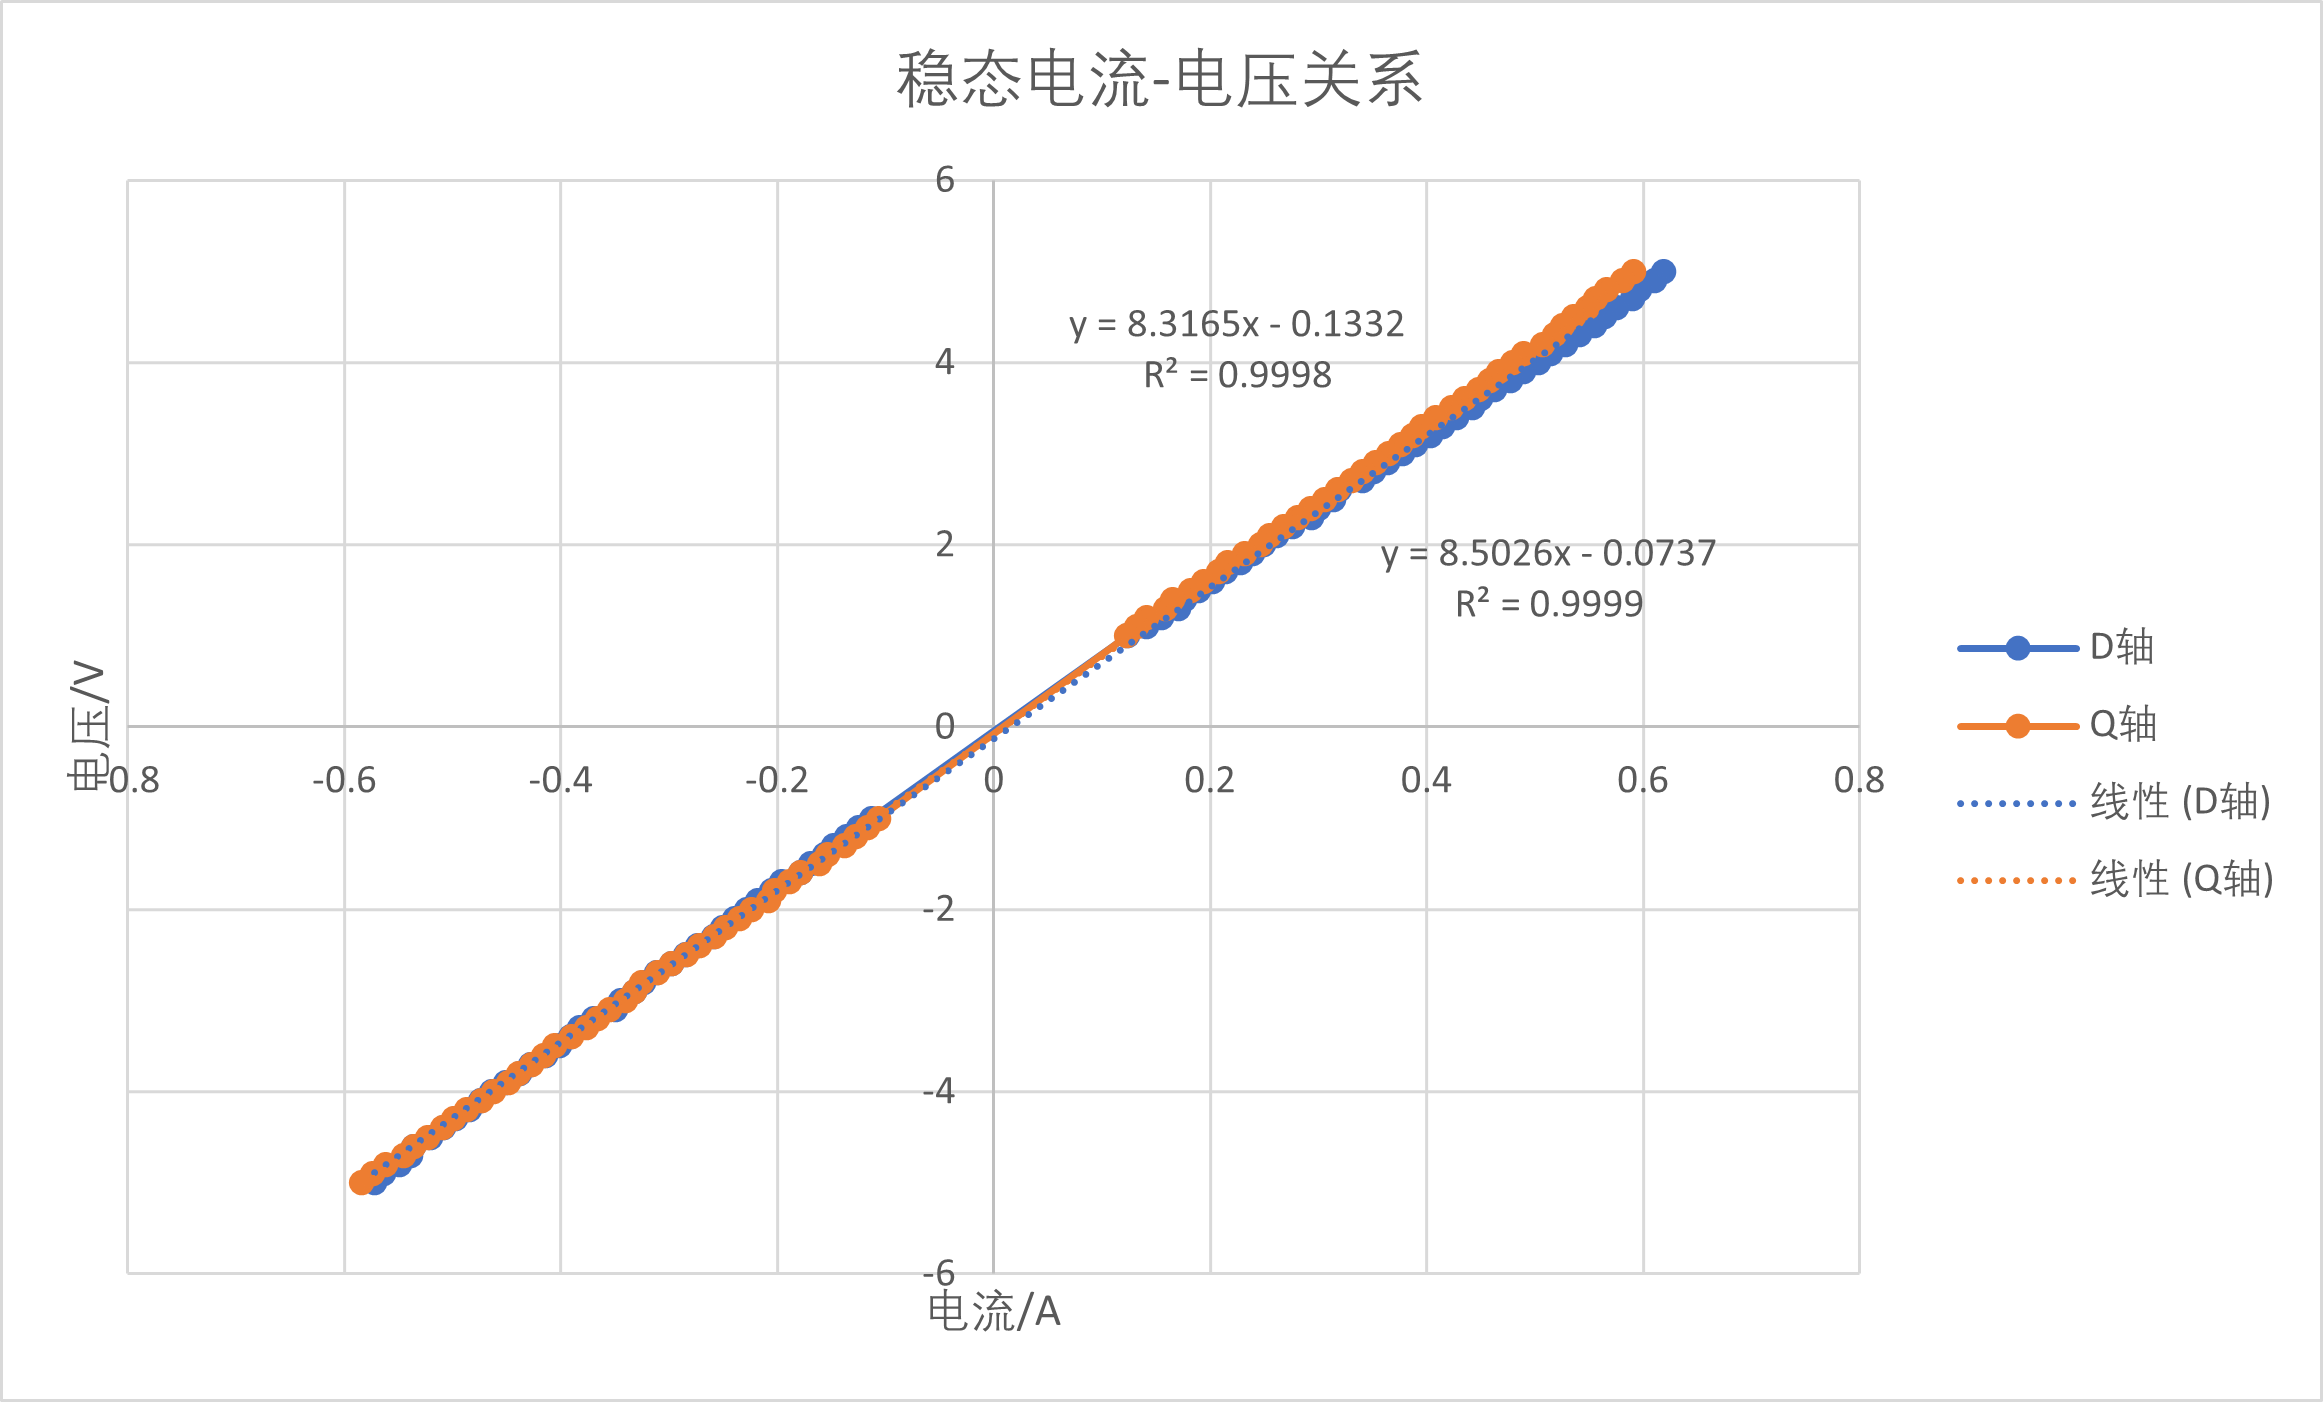
\includegraphics[width=0.6\textwidth]
    {图片/相电阻辨识曲线.png}
    \caption{相电阻辨识曲线}
\end{figure}

D轴拟合稳态电压电流关系式为\(U_d = 5.713I_d-0.0885\)，决定系数\(R_D^2=0.9999\)；
Q轴拟合稳态电压电流关系式为\(U_q = 5.6895I_q+0.0753\)，决定系数\(R_Q^2=0.9999\)。
两者平均可得相电阻辨识结果为
\begin{equation*}
    R_{sO}=5.70125\Omega
\end{equation*}

\subsection{基于相间电感测量的同步电感估测}

为了方便对后续同步电感测量结果进行判断，这里首先进行基于相间电感的同步电感估测。
对于永磁同步电机，在自然坐标系A-B-C下，每一相的自感和互感满足如下两式：

\begin{minipage}{0.5\textwidth}
    \begin{equation*}
        \begin{cases}
            L_A=L_{s0}-L_{s2}\cos2\theta_e\\
            L_B=L_{s0}-L_{s2}\cos(2\theta_e-\cfrac{4\pi}{3})\\
            L_C=L_{s0}-L_{s2}\cos(2\theta_e+\cfrac{4\pi}{3})
        \end{cases}
    \end{equation*}
\end{minipage}
\begin{minipage}{0.5\textwidth}
    \begin{equation*}
        \begin{cases}
            M_{AB}=M_{BA}=M_{s0}-M_{s2}\cos(2\theta_e+\cfrac{4\pi}{3})\\
            M_{BC}=M_{CB}=M_{s0}-M_{s2}\cos2\theta_e\\
            M_{AC}=M_{CA}=M_{s0}-M_{s2}\cos(2\theta_e-\cfrac{4\pi}{3})
        \end{cases}
    \end{equation*}
\end{minipage}

相间电感测量的具体步骤为：将一相开路，使用LCR电桥测量从另外两相看进去得到的等效电感。LCR电桥测量原理是注入恒定幅值和频率的
电压正弦波，通过稳态正弦电流响应，分析幅值和相位偏差，进而得到等效阻抗。因此测量电感可以表示为\(L=\cfrac{d\psi}{di}\)，其中
\(\psi\)表示等效磁链。

以C相开路，从AB相看进去测量相间电感为例。设此时\(i_A=i\)，则\(i_B=-i\)而\(i_C=0\)。根据磁链的定义式，可得A相磁链\(\psi_A\)和B
相磁链\(\psi_B\)的表达式为：
\begin{equation*}
    \begin{cases}
        \psi_A=L_Ai_A+M_{BA}i_B+M_{CA}i_C=(L_{s0}-L_{s2}\cos2\theta_e)i+
        (M_{s0}-M_{s2}\cos(2\theta_e+\cfrac{4\pi}{3}))(-i)\\
        \psi_B=L_Bi_B+M_{AB}i_A+M_{CB}i_C=(L_{s0}-L_{s2}\cos(2\theta_e-\cfrac{4\pi}{3}))(-i)+
        (M_{s0}-M_{s2}\cos(2\theta_e+\cfrac{4\pi}{3}))i
    \end{cases}
\end{equation*}

从AB之间看进去的等效磁链为\(\psi_{AB}=\psi_A-\psi_B\)。带入可得：
\begin{equation*}
    \psi_{AB}=2(L_{s0}-M_{s0})i
    -iL_{s2}(\cos2\theta_e+\cos(2\theta_e-\cfrac{4\pi}{3}))
    +iM_{s2}(\cos(2\theta_e+\cfrac{4\pi}{3})+\cos(2\theta_e+\cfrac{4\pi}{3}))
\end{equation*}

测量得到的电感表达式为\(L_{AB}=\cfrac{d\psi_{AB}}{di}\)，代入可得：
\begin{equation*}
    L_{AB}=2(L_{s0}-M_{s0})
    -L_{s2}(\cos2\theta_e+\cos(2\theta_e-\cfrac{4\pi}{3}))
    +M_{s2}(\cos(2\theta_e+\cfrac{4\pi}{3})+\cos(2\theta_e+\cfrac{4\pi}{3}))
\end{equation*}

化简可得：
\begin{equation*}
    L_{AB}=2(L_{s0}-M_{s0})+(L_{s2}+2M_{s2})\cos(2\theta_e-\cfrac{2\pi}{3})
\end{equation*}

结合同步电感定义式\eqref{eq:同步电感定义式}如下：
\begin{equation*}
    \begin{cases}
        L_d=L_{s0}-M_{s0}-\cfrac{L_{s2}}{2}-M_{s2}\\
        L_q=L_{s0}-M_{s0}+\cfrac{L_{s2}}{2}+M_{s2}
    \end{cases}
\end{equation*}

可得AB相间电感表达式为：
\begin{equation*}
    L_{AB}=(L_d+L_q)+(L_q-L_d)\cos(2\theta_e-\cfrac{2\pi}{3})
\end{equation*}

同理可得BC和AC相间电感表达式，结合AB相间电感表达式可得：
\begin{equation}
    \begin{cases}
        L_{AB}=(L_d+L_q)+(L_q-L_d)\cos(2\theta_e-\cfrac{2\pi}{3})
        \\
        L_{BC}=(L_d+L_q)+(L_q-L_d)\cos2\theta_e
        \\
        L_{AC}=(L_d+L_q)+(L_q-L_d)\cos(2\theta_e+\cfrac{2\pi}{3})
    \end{cases}
    \label{eq:相间电感表达式}
\end{equation}

因此可以通过测量相间电感随电角度变化的曲线幅值和平均值，来估测同步电感\(L_d=\cfrac{L_{\min}}{2}\)和\(L_q=\cfrac{L_{\max}}{2}\)。
在不同频率下测量相间电感曲线如下图所示（样本数为36）。
\begin{figure}[H]
    \begin{minipage}{0.5\textwidth}
        \centering
        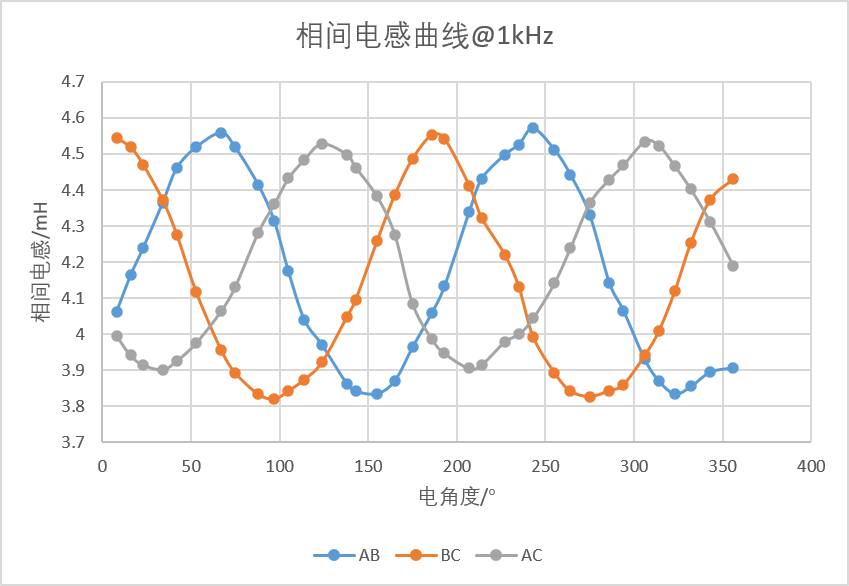
\includegraphics[width=\textwidth]{图片/1kHz相间电感测量曲线.png}
        \caption{1kHz相间电感测量曲线}
    \end{minipage}
        \begin{minipage}{0.5\textwidth}
        \centering
        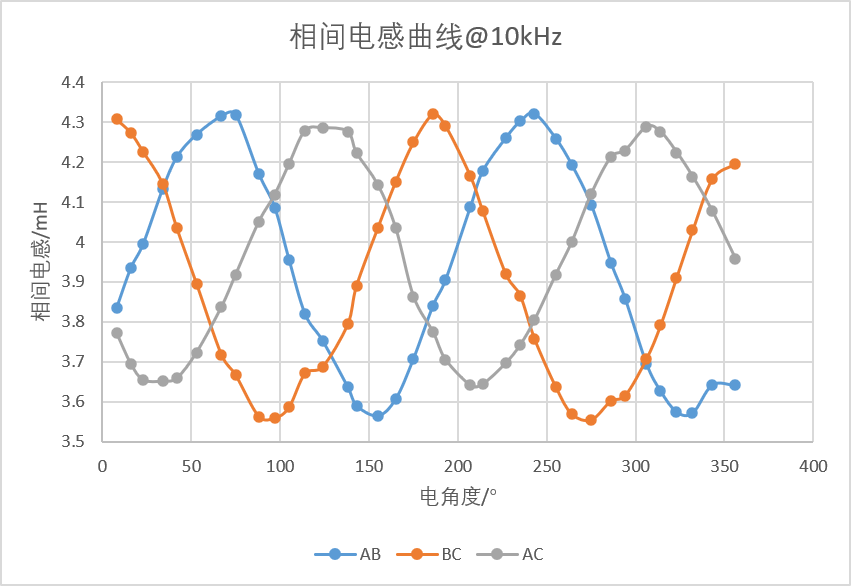
\includegraphics[width=\textwidth]{图片/10kHz相间电感测量曲线.png}
        \caption{10kHz相间电感测量曲线}
    \end{minipage}
\end{figure}

根据线性回归知识，若某输出与多个输入满足线性关系\(y=a_0+\sum\limits_{i=1}^ma_mx_m\)，则进行n次测量后
定义输出数据向量\(Y=\begin{bmatrix}y_1\\y_2\\\vdots\\y_n\end{bmatrix}_{n\times 1}\)和输入数据矩阵
\(X=\begin{bmatrix}
    1&x_{11}&x_{12}&\cdots&x_{1m}\\1&x_{21}&x_{22}&\cdots&x_{2m}\\\vdots&\vdots&\vdots&\ddots&\vdots\\1&x_{n1}&x_{n2}&\cdots&x_{nm}
\end{bmatrix}_{n\times(m+1)}\)，并且有待定系数矩阵\(A=\begin{bmatrix}a_0\\a_1\\a_2\\\vdots\\a_m\end{bmatrix}_{(m+1)\times 1}\)。那么理想情况下
满足\(Y=XA\)，而由于噪声和测量误差存在，实际上各个数据满足\(Y=XA+\varepsilon\)。

经典的最小二乘拟合方法要求将所有数据的残差平方和最小，即损失函数为\(S(A)=(Y-XA)^T(Y-XA)\)。
展开可得\(S(A)=Y^TY-Y^TXA-A^TX^TY+A^TX^TXA\)，其中根据维度分析可知\(Y^TXA=A^TX^TY\)为标量，因此
损失函数可以写为\(S(A)=Y^TY+A^TX^TXA-2A^TX^TY\)。

求解损失函数梯度为\(\cfrac{\partial S(A)}{\partial A}=2X^TXA-2X^TY\)。令其为零求解使得损失函数最小的系数矩阵表达式为：
\begin{equation}
    \hat{A}=(X^TX)^{-1}X^TY。
    \label{eq:多元线性回归公式}
\end{equation}

这也就是多元线性回归的参数计算公式。根据相间电感表达式\eqref{eq:相间电感表达式}可知，任意两相之间的测量电感可以一般地表示为
\begin{equation*}
    L=a_0+a_1\cos2\theta_e+a_2\sin2\theta_e
\end{equation*}

将\(\cos2\theta_e\)和\(\sin2\theta_e\)视为两个输入，则可以通过多元线性回归计算最小二乘拟合参数。拟合结果如下图所示。
\begin{figure}[H]
    \begin{minipage}{0.5\textwidth}
        \centering
        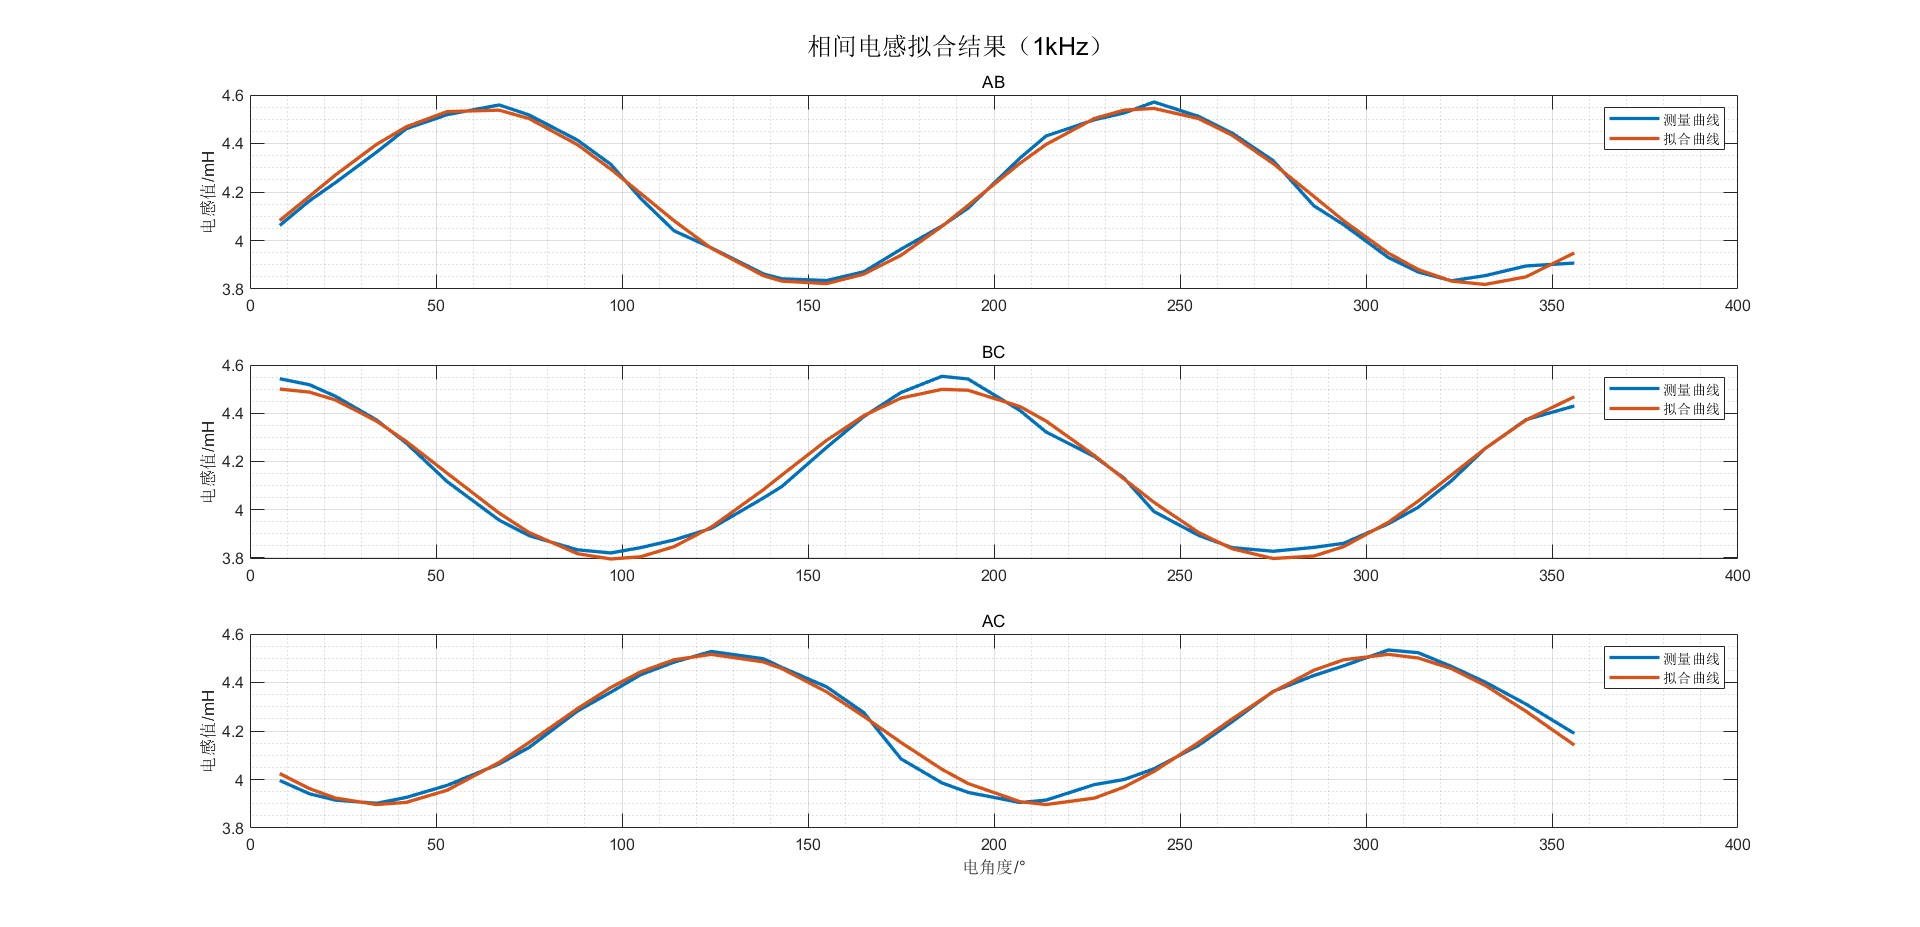
\includegraphics[width=\textwidth]{图片/1kHz相间电感拟合结果.jpg}
        \caption{1kHz相间电感拟合结果}
    \end{minipage}
        \begin{minipage}{0.5\textwidth}
        \centering
        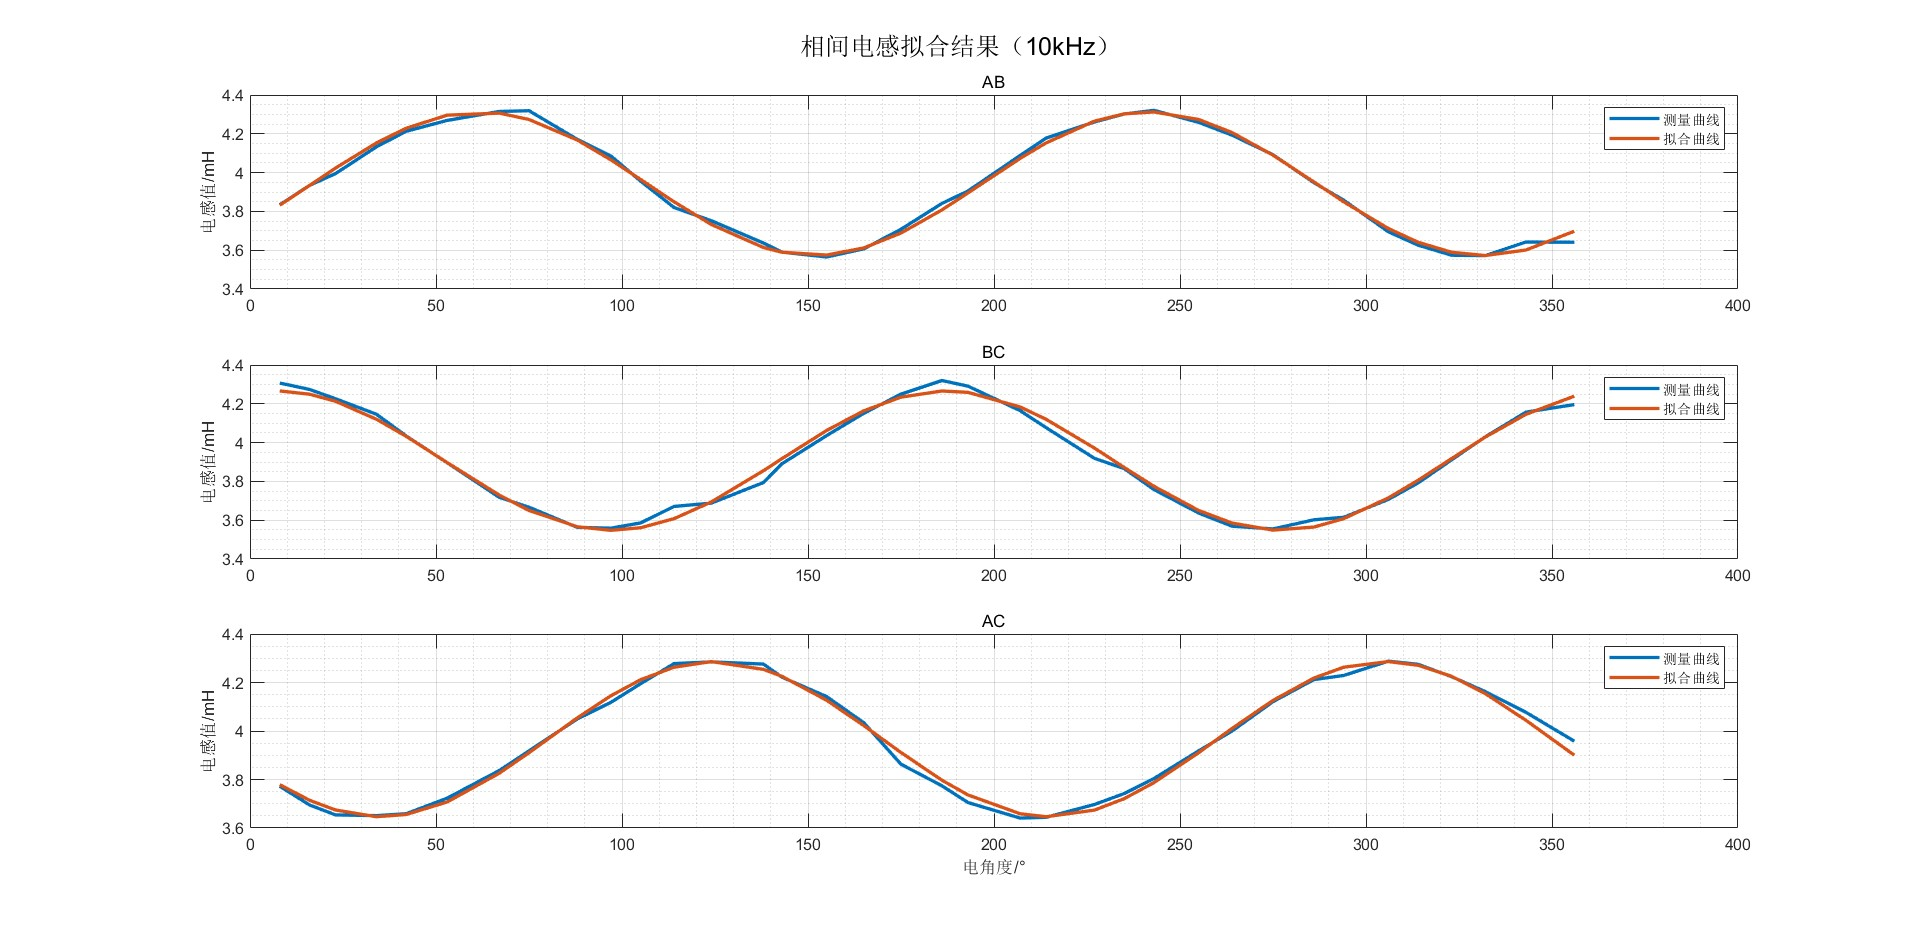
\includegraphics[width=\textwidth]{图片/10kHz相间电感拟合结果.jpg}
        \caption{10kHz相间电感拟合结果}
    \end{minipage}
\end{figure}

线性回归为：
\begin{table}[H]
    \centering
    \begin{tabular}{|c|c|c|c|}
        \hline
        测试条件&拟合结果&决定系数\(R^2\)&调整决定系数\(R^2_{adj}\)\\
        \hline
        AB@1kHz&
        \(\begin{aligned}L &= 4.1821-0.19224\cos2\theta_e+0.30851\sin2\theta_e\\
        &=4.1821+0.3635\cos(2\theta_e-121.93°)\end{aligned}\)
        &0.99242&0.99196\\
        \hline
        BC@1kHz&
        \(\begin{aligned}L &= 4.1473+0.33811\cos2\theta_e+0.10075\sin2\theta_e\\
        &=4.1473+0.3528\cos(2\theta_e-16.594°)\end{aligned}\)
        &0.98795&0.98722\\
        \hline
        AC@1kHz&
        \(\begin{aligned}L &= 4.2064-0.10595\cos2\theta_e-0.29117\sin2\theta_e\\
        &=4.2064+0.30985\cos(2\theta_e+109.99°)\end{aligned}\)
        &0.98689&0.98610\\
        \hline
        AB@10kHz&
        \(\begin{aligned}L &= 3.9427-0.20384\cos2\theta_e+0.30907\sin2\theta_e\\
        &=3.9427+0.37024\cos(2\theta_e-123.41°)\end{aligned}\)
        &0.99367&0.99329\\
        \hline
        BC@10kHz&
        \(\begin{aligned}L &= 3.9071+0.34803\cos2\theta_e+0.089177\sin2\theta_e\\
        &=3.90717+0.35927\cos(2\theta_e-14.372°)\end{aligned}\)
        &0.98844&0.98774\\
        \hline
        AC@10kHz&
        \(\begin{aligned}L &= 3.9664-0.10916\cos2\theta_e-0.3009\sin2\theta_e\\
        &=3.9664+0.32009\cos(2\theta_e+109.94°)\end{aligned}\)
        &0.99228&0.99181\\
        \hline
    \end{tabular}
    \caption{多元线性回归表}
    \label{tab:多元线性回归表}
\end{table}
根据回归结果分析，每组的决定系数\(R^2\)
\footnote{决定系数\(R^2\)定义为 \(1-\cfrac{SSE}{SST}\)，其中SSE为残差平方和\(\sum\limits_{i=1}^n(\hat{y}_i-y_i)^2\)，
SST表示总平方和\(\sum\limits_{i=1}^n(y_i-\bar{y})^2\)，分别表示“回归可解释的异变”和“总异变度”，是进行线性回归
结果评估的典型标准。}
和根据样本进行的调整决定系数\(R^2_{adj}\)
\footnote{调整决定系数定义为 \(1-\cfrac{SSE}{SST}\times\cfrac{n-1}{n-k-1}\)，其中n表示总样本量，k表示
待估计参数个数，主要是为了修正决定系数会随着待估计参数个数升高而自然升高的问题。}
均不小于0.98，线性回归的效果好。

接下来计算估计的\(L_d\)和\(L_q\)。在多元线性回归中的残差\(\varepsilon = Y - XA\)认为是服从正态分布的，即\(\varepsilon\sim N(0,\sigma^2)\)，
那么其方差的无偏估计为\(\hat{\sigma^2} = \cfrac{SSE}{n-k}\)，其中SSE表示残差的平方和，n为样本个数（此处为36），而
k为待估计参数个数（此处为3）。使用n-k而不是n是因为数据本身估计了k个参数，真正的随机信息只有n-k个维度。

根据多元线性回归公式\eqref{eq:多元线性回归公式}，将理论值\(Y=XA+\varepsilon\)代入可得：
\begin{equation*}
    \begin{aligned}
        \hat{A} &= (X^TX)^{-1}X^T(XA+\varepsilon)\\
        &=(X^TX)^{-1}X^TXA+(X^TX)^{-1}X^T\varepsilon\\
        &= A + (X^TX)^{-1}X^T\varepsilon
    \end{aligned}
\end{equation*}

由于残差服从正态分布，根据上式可知估计参数也应服从多元正态分布，数学推导可知其服从\(\hat{A}\sim N(A,\sigma^2(X^TX)^{-1})\)
，其中\(\sigma^2(X^TX)^{-1}\)为协方差矩阵。由于残差的真实方差\(\sigma^2\)未知，因此用上文计算得到的
残差方差的无偏估计\(\hat{\sigma^2} = \cfrac{SSE}{n-k}\)代替，即估计参数的协方差矩阵为
\(C = \hat{\sigma^2}X^TX^{-1}\)。根据误差的传递公式，对于某个变量\(y=f(x_1,x_2,\cdots,x_n)\)，
若已知输入变量的标准差\(\sigma_{x_i}\)和测量值\(x_i\)，则可以估计输出的测量值为
\(\hat{y}=f(x_1,\cdots,x_n)\)和标准差\(\sigma_y=\sqrt{(\nabla f)^T C (\nabla f)}\)。

针对拟合结果\(L=a_0+a_1\cos2\theta_e+a_2\sin2\theta_e\)，结合相间电感公式\eqref{eq:相间电感表达式}可以得到
\(L_d,L_q\)的计算式为：
\begin{equation*}
    \begin{cases}
        L_d =\cfrac{a_0-\sqrt{a_1^2+a_2^2}}{2}\\
        L_q =\cfrac{a_0+\sqrt{a_1^2+a_2^2}}{2}
    \end{cases}
\end{equation*}

两者的梯度为：

\begin{minipage}{0.5\textwidth}
    \begin{equation*}
        \nabla L_d =\begin{bmatrix}\cfrac{1}{2}\\-\cfrac{a_1}{2\sqrt{a_1^2+a_2^2}}\\
        -\cfrac{a_2}{2\sqrt{a_1^2+a_2^2}}\end{bmatrix}
    \end{equation*}
\end{minipage}
\begin{minipage}{0.5\textwidth}
    \begin{equation*}
        \nabla L_q =\begin{bmatrix}\cfrac{1}{2}\\
        \cfrac{a_1}{2\sqrt{a_1^2+a_2^2}}\\
        \cfrac{a_2}{2\sqrt{a_1^2+a_2^2}}\end{bmatrix}
    \end{equation*}
\end{minipage}

计算可得各组的估计\(L_d,L_q\)和标准差为：
\begin{table}[H]
    \centering
    \begin{tabular}{|c|c|c|c|c|}
        \hline
        测试条件&\(L_d\)估计值&\(L_d\)标准差&\(L_q\)估计值&\(L_q\)标准差\\
        \hline
        AB@1kHz&
        1.90928&0.00337&2.27278&0.00338\\
        \hline
        BC@1kHz&
        1.89725&0.00415&2.25006&0.00417\\
        \hline
        AC@1kHz&
        1.94828&0.00383&2.25813&0.00381\\
        \hline
        AB@10kHz&
        1.78625&0.00313&2.15649&0.00315\\
        \hline
        BC@10kHz&
        1.77392&0.00414&2.13319&0.00415\\
        \hline
        AC@10kHz&
        1.82315&0.00303&2.14324&0.00301\\
        \hline
    \end{tabular}
    \caption{估计结果和标准差}
    \label{tab:估计结果和标准差}
\end{table}

从估计值来看，在10kHz下测量的结果明显小于在1kHz下测量的结果，
这是高频信号趋肤效应
\footnote{频率较高时，电流会集中在导体的表面，而不会进入导体内部。趋肤效应会导致内磁链降低，等效电感
降低。}、铁芯涡流损耗
\footnote{交变磁通在铁芯中感应涡流，产生去磁效应，等效于在电感两端并联了随频率升高而降低的涡流电阻，
导致表观电感下降。}等效应的综合作用结果。而标准差相较于估计值的百分比不超过\(0.2\%\)，整体极小，
而发现不同相间测量组的估计值相差超过可达0.05mH，远大于标准差的0.003mH，这说明
存在无法被正态分布所解释的系统误差。

此外，相间电感测量是在单频点上进行的分析，而后续使用的Ho-Kalman辨识算法是典型的最小子空间辨识算法，
是在宽频带上进行的辨识算法，两者在参数的测量辨识原理上存在本质的不同。
\footnote{Ho-Kalman辨识是对时域Hankel矩阵的低秩逼近，最小化时域误差，用帕塞瓦尔定理可以等效为
对频域能量的加权最小二乘拟合，即寻求能够最小化频域能量残差平方和的传递函数。这其中
的权重隐含在系统响应中，响应能量越强的频段拥有更大的权重。这使得在各个频点上的权重不止依赖于输入信号，
也依赖于待测系统本身。在宽频带信号和脉动磁场作用下，涡流损耗加剧，使
得\(L_d\)和\(L_q\)相较于LCR电桥的准静止测量有较大的变化，而DQ轴磁路不同，
两者的饱和特性与动态响应天然存在差异。在上述情况下Ho-Kalman辨识算法往往与LCR测量结果
有较大差异。此外，Ho-Kalman对象不是只有电机，也包含逆变器等其他非理想因素，这些因素却恰恰是
实际控制中必须考虑的。因此LCR测量的分析结果只能作为简单的电感数量级、相对关系、凸极率分析，不可作为
实际控制设计参数。}

综上所述，选取六组的平均值±0.5倍极差作为同步电感的LCR测量估计结果：
\begin{equation*}
    \begin{cases}
        L_d\in(1.76917,1.94354)\textrm{mH}
        \\
        L_q\in(2.13252,2.27211)\textrm{mH}
    \end{cases}
\end{equation*}

\subsection{辨识算法的仿真分析}
在正式进入实际测量之前，在本小节搭建仿真模型，以此来分析辨识结果的可靠程度。取相对误差5\(\%\)为可接受范围进行分析。

\subsubsection{辨识算法概述}

对于电机的电路方程\eqref{eq:同步坐标系下电路方程}如下所示：
\begin{equation}
    \begin{bmatrix}
        u_d\\u_q
    \end{bmatrix}
    =\begin{bmatrix}R_s&-\omega_eL_q\\\omega_eL_d&R_s\end{bmatrix}
    \begin{bmatrix}i_d\\i_q\end{bmatrix}
    +\begin{bmatrix}L_d&0\\0&L_q\end{bmatrix}
    \begin{bmatrix}\dot{i}_d\\\dot{i}_q\end{bmatrix}
    +\begin{bmatrix}0\\\psi_m\omega_e\end{bmatrix}
    \tag{\ref{eq:同步坐标系下电路方程}}
\end{equation}

若能够通过特定手段使得交叉耦合项\(\omega_e L_qi_q\)和\(\omega_e(L_di_q+\psi_m)\)归零，则DQ轴电路方程可以简化为：
\begin{equation*}
    \begin{cases}
        u_d=R_si_d+L_d\cfrac{di_d}{dt}\\
        u_q=R_si_q+L_q\cfrac{di_q}{dt}
    \end{cases}
\end{equation*}

两边取拉普拉斯变换，得到DQ轴电压到电流的传递函数为\(G_D(s)=\cfrac{1}{R_s+L_ds}\)和\(G_Q(s)=\cfrac{1}{R_s+L_qs}\)。
极点分别位于\(s_{pD}=-\cfrac{R_s}{L_d}\)和\(s_{pQ}=-\cfrac{R_s}{L_q}\)均为一阶系统。

针对一阶系统的辨识，这里采用Ho-Kalman辨识方法（下称HK辨识法）。该方法的数学基础（凯莱-哈密顿定理、脉冲响应序列与马尔科夫系数、
汉克尔矩阵的构造与奇异值分解、最小状态空间实现）详见\ref{sec:Ho-Kalman辨识过程介绍}，此处仅给出算法流程概要和与本文应用直接相关的结论。

HK辨识法的基本步骤为：
\begin{itemize}
    \item 计算输入信号的自相关序列和输入输出信号的互相关序列，根据维纳-霍普夫方程求解系统的脉冲响应序列
    \item 根据脉冲响应序列构造汉克尔矩阵
    \item 对汉克尔矩阵进行奇异值分解，确定系统的阶次
    \item 根据系统阶次进行奇异值截断，结合汉克尔矩阵、移位汉克尔矩阵和奇异值，求解系统的最小状态空间实现
    \item 根据最小状态空间实现求解传递函数
\end{itemize}

其中，汉克尔矩阵的阶次一般选取到脉冲响应序列暂态响应基本完成处，确保囊括所有独立信息，同时避免引入信噪比极低的稳态数据造成误判。

连续域下传递函数的极点为\(s_{pD}=-\cfrac{R_s}{L_d}\)和\(s_{pQ}=-\cfrac{R_s}{L_q}\)。
经过脉冲采样，即零阶保持变换后，离散域极点
位于\(z_{pD}=e^{-T_s\frac{R_s}{L_d}}\)和\(z_{pQ}=e^{-T_s\frac{R_s}{L_q}}\)，其中\(T_s\)为采样周期。
因此辨识结果可以计算为\(L_d=-\cfrac{T_sR_s}{\ln(z_{pD})}\)和\(L_q=-\cfrac{T_sR_s}{\ln(z_{pQ})}\)。

\subsubsection{仿真模型搭建}
在Simulink中搭建仿真模型如下图所示。
\begin{figure}[H]
    \centering
    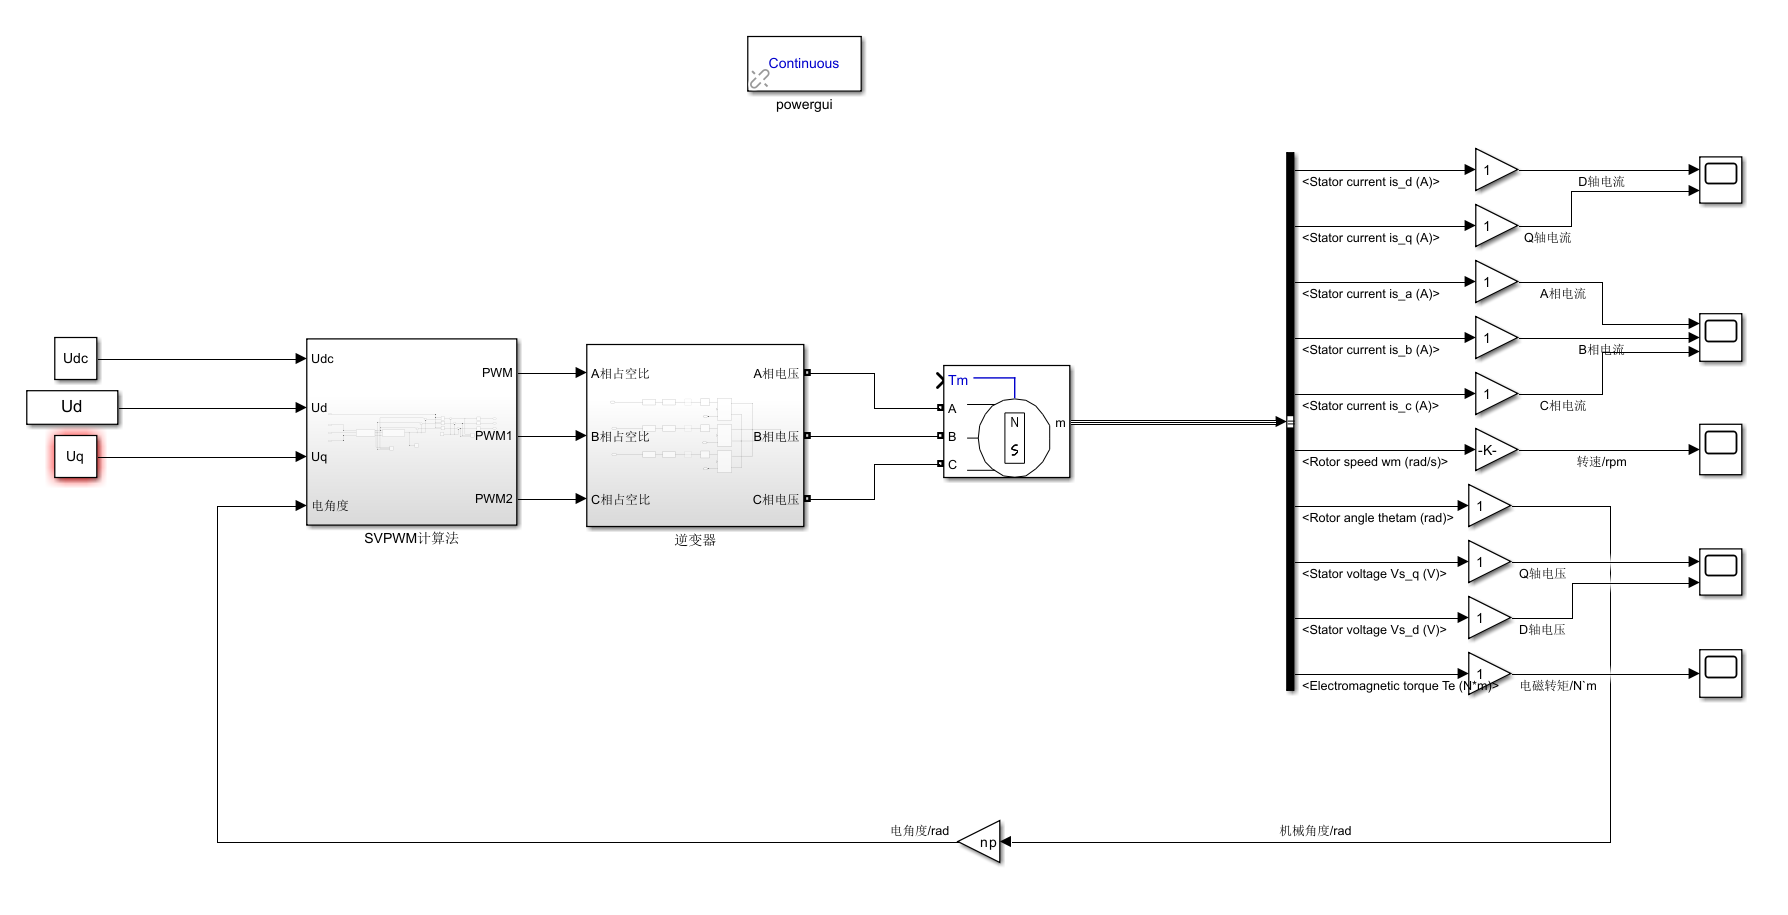
\includegraphics[width=0.8\textwidth]
    {图片/仿真模型.png}
    \caption{仿真模型}
\end{figure}

设定电机参数为相电阻\(R_s=8\Omega\)，同步电感\(L_d=2\)mH，\(L_q=2.5\)mH，永磁体磁链\(\psi_m=0.01\)Wb，极对数\(n_p=14\)，
母线电压\(12\)V。采用SVPWM调制，PWM频率为\(15\)kHz。

对于伪随机信号的选取，选择级数N=11，Hanekel矩阵阶次为8，幅值为1V，采样周期\(T_s=1/15000=66.67\)us。

在系统阶次的选择上，由于理想电路模型本身为一阶，因此系统阶次选取为1。但是PWM和逆变器本身会引入时延，会使得辨识阶次升高至2。接下来对此
简单进行分析。

对于SVPWM调制方法，会引入1拍的延迟，也就是有\(\tau\approx\)66.67us。
根据采用的三相全桥芯片DRV8313数据手册动态特性相关表述，如下所示，DRV8313的行为近似为纯时延+一阶惯性环节。
\begin{figure}[H]
    \centering
    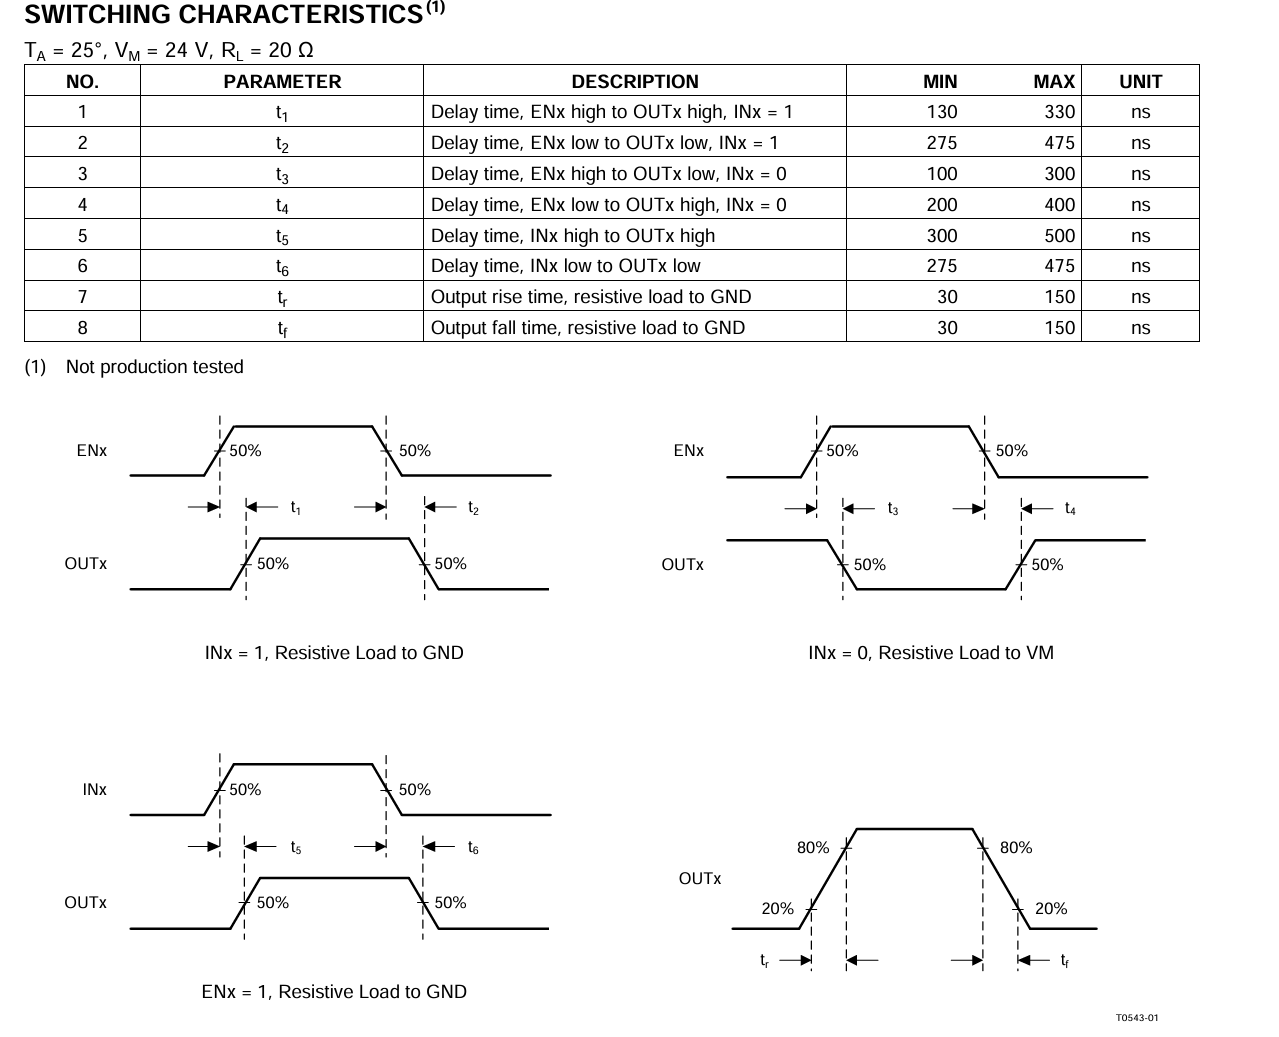
\includegraphics[width=0.8\textwidth]
    {图片/DRV8313动态特性.png}
    \caption{DRV8313动态特性}
\end{figure}

用示波器测量PWM输出信号和逆变器输出时序波形如下图所示。分析可知DRV8313时延时间约260ns，时间常数约120ns。
\begin{figure}[H]
    \begin{minipage}{0.5\textwidth}
        \centering
        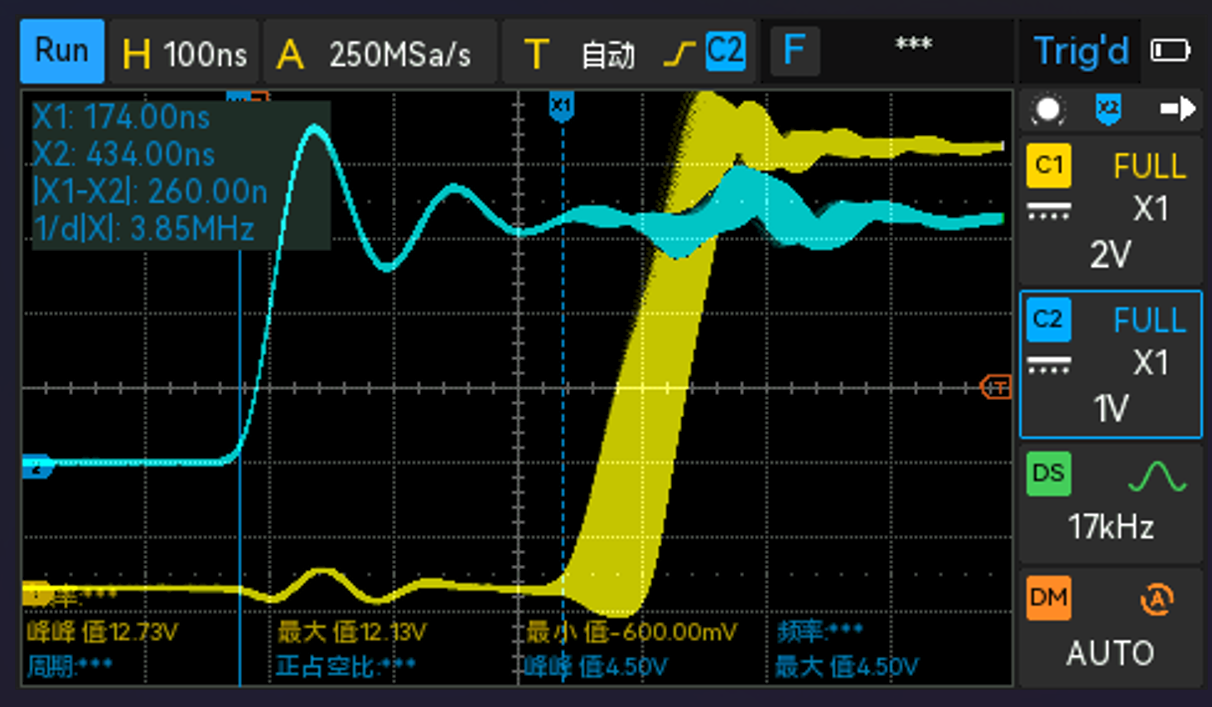
\includegraphics[width=\textwidth]
        {图片/DRV8313动态特性波形图（延时测量）.png}
        \caption{DRV8313逆变器输出时序波形（延时）}
    \end{minipage}
    \begin{minipage}{0.5\textwidth}
        \centering
        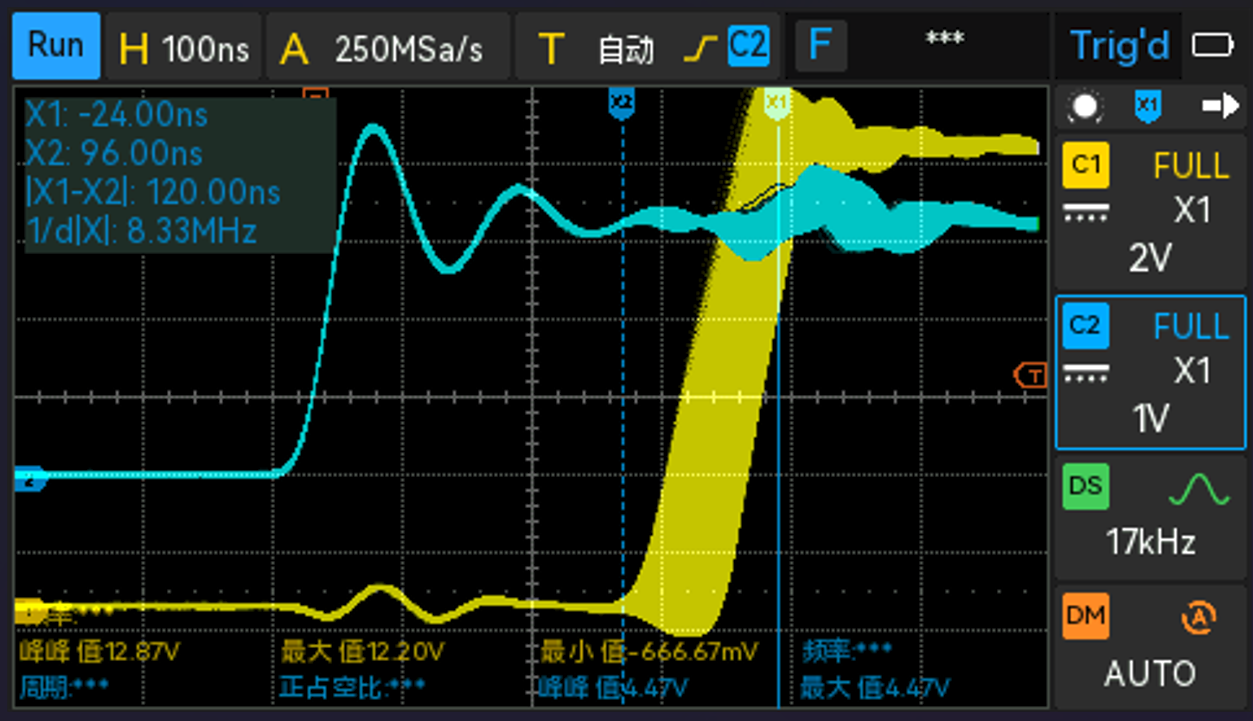
\includegraphics[width=\textwidth]
        {图片/DRV8313动态特性波形图（惯性测量）.png}
        \caption{DRV8313逆变器输出时序波形（惯性）}
    \end{minipage}
\end{figure}

因此PWM和逆变器的传递函数可以表示为：
\begin{equation*}
    \begin{aligned}
        G(s)&=e^{-(66.67\times10^{-6})s}\times e^{-(260\times 10^{-9})s}
        \cfrac{1}{120\times 10^{-9}s+1}\\
        &=e^{-66.93\times10^{-6}s}\cfrac{1}{120\times 10^{-9}s+1}
    \end{aligned}
\end{equation*}

此时整体的被控对象可以表示为\(G(s)=\cfrac{1}{R+Ls}\times\cfrac{1}{120\times 10^{-9}s+1}
\times e^{-66.93\times10^{-6}s}\)，而采样周期\(T_s = 66.67\times 10^{-6}\)s，存在分数拍滞后，
需要用修正Z变换分析其在离散域中的传递函数。但根据Z变换的相关知识可知，修正Z变换只会引起零点和直流
增益的变化。此外，如果只关注极点，则\(\mathcal{Z}[G_1(s)G_2(s)]\)和\(\mathcal{Z}[G_1(s)]\mathcal{
G_2(s)}\)的极点是一致的。因此尽管考虑PWM和逆变器带来的滞后，对于同步电感的辨识仍可以用
\(L_d=-\cfrac{T_sR_s}{\ln(z_{pD})}\)和\(L_q=-\cfrac{T_sR_s}{\ln(z_{pQ})}\)来计算。只是由于
PWM和逆变器带来的非理想因素会导致系统阶次升高，引入极高频的快极点，此时需要进行极点模态分离。

在仿真模型中，用PWM初始延迟模拟PWM的一拍滞后，用时延+惯性环节模拟逆变器特性，并将其与无时延的结果进行对比。
含时延时系统阶次选择为2阶，不含时延时系统阶次选择为1阶。而对于二阶系统，进行模态分离，选取靠近单位圆的慢极点，
将其视为电机本身Q轴电路的模态，而靠近原点的极点视为PWM和逆变器时延引入的模态。

此外，为了模拟实际的非理想因素，还会再输出端引入白噪声模拟采样噪声。后续的仿真分析，将在考虑PWM时延、逆变器惯性
和采样噪声的非理想状态，和不考虑PWM时延、逆变器惯性和采样噪声理想状态都进行分析，并进行对比分析。

\subsubsection{D轴同步电感辨识仿真}

根据电磁转矩表达式\(T_e=\cfrac32pi_qi_d(L_d-L_q)+\cfrac32\psi_mpi_q\)可知，若\(i_q=0\)，则不会产生电磁转矩，电机不会转动，
D轴电路方程可以表示为\(u_d = R_si_d+L_d\cfrac{di_d}{dt}\)。而在零初始条件下，根据电路方程，能够激起\(i_q\)变化的唯一方法是
给定非零的\(u_q\)。因此，只在D轴注入电压，交叉耦合项\(\omega_eL_qi_q=0\)，D轴电路维持为线性定常系统。

首先在理想状态下（不考虑PWM时延、逆变器惯性和采样噪声），在D轴工作点0V附近进行HK辨识仿真，结果如下所示。
\begin{figure}[H]
    \begin{minipage}{0.5\textwidth}
        \centering
        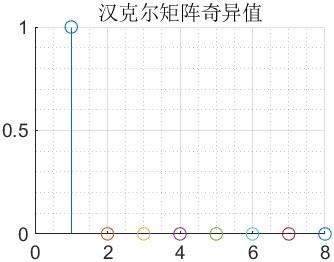
\includegraphics[width=\textwidth]
        {图片/D轴工作点0V归一化奇异值分解图（仿真，理想状态）.jpg}
        \caption{D轴工作点0V归一化奇异值分解图（仿真，理想状态）}
    \end{minipage}
    \begin{minipage}{0.5\textwidth}
        \centering
        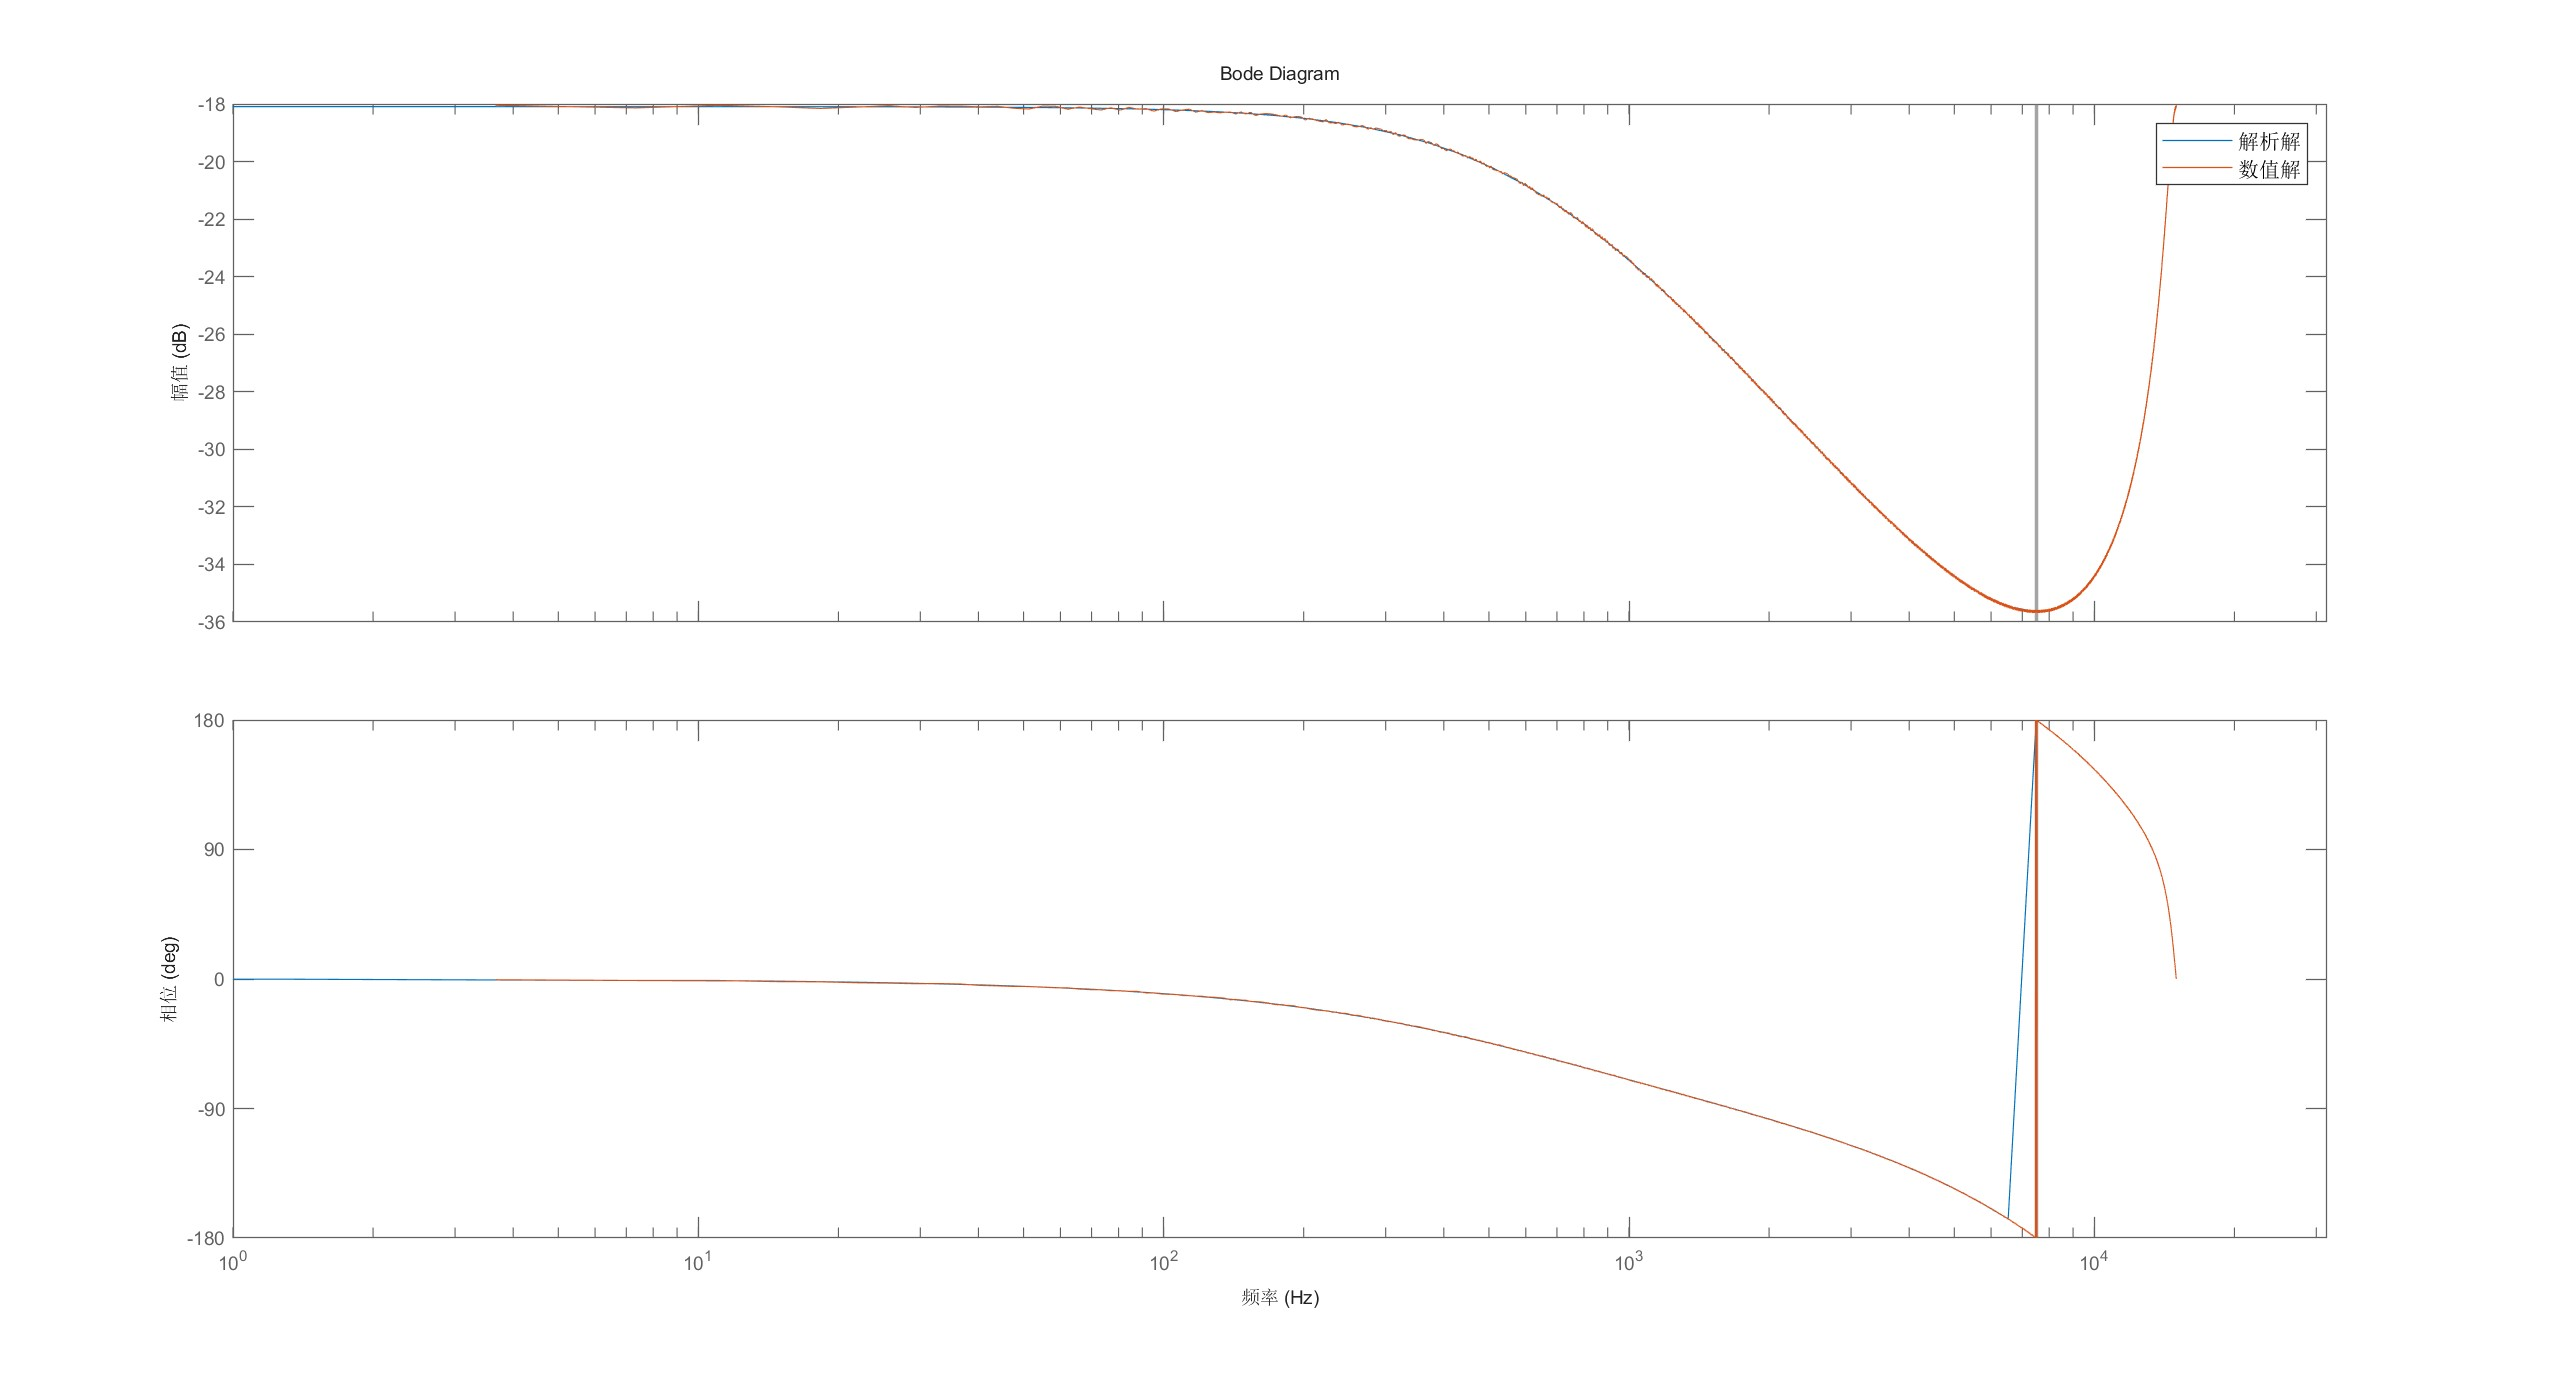
\includegraphics[width=\textwidth]
        {图片/D轴工作点0V解析解与数值解频域对比图（仿真，理想状态）.jpg}
        \caption{D轴工作点0V解析解与数值解频域对比图（仿真，理想状态）}
    \end{minipage}
\end{figure}

可以发现，归一化后的奇异值分解显示系统为一阶，与推导的结果一致。辨识传递函数为：
\begin{equation*}
    G_D(z)=\cfrac{2.125\times 10^{-6} + 0.02916z^{-1}}{1 - 0.7659z^{-1}}
\end{equation*}

数值解与解析解的幅频相关系数
\footnote{皮尔逊相关系数定义为\(r=\cfrac{\sum\limits_{i=1}^n(x_i-\bar{x})(y_i-\bar{y})}
{\sqrt{\sum\limits_{i=1}^n(x_i-\bar{x})^2\sum\limits_{i=1}^n(y_i-\bar{y})^2}}\)，用于描述
两组数据之间的线性相关程度，取值范围为[-1,1]。在一元线性回归中相关系数和决定系数满足\(R^2=r^2\)。
这里衡量的两组原则上一致的数据的线性相关程度，因此相关系数越接近1越好。}
为99.9165\(\%\)，相频相关系数为99.99136\(\%\)，拟合优度
\footnote{拟合优度定义为\(\textrm{BFT}=1-\cfrac{\|y-\hat{y}\|}{\|y-\bar{y}\|}\)，
其中\(y\)表示实测数据，\(\hat{y}\)表示仿真和估测数据，而\(\|\cdot\|\)表示欧几里得范数，对于实数向量
计算为\(\|x\|=\sqrt{\sum\limits_{i=1}^nx_i^2}\)，
对于复数则计算为\(\|z\|=\sqrt{\sum\limits_{i=1}^n|z_i|^2}\)，相较于相关系数，拟合优度
能够反映两组数据的一致性，对直流偏置、线性增益有敏感性，同样也是越接近1两组数据的一致性越高。}
97.49761\(\%\)，
拟合程度极高。
解析解极点位于\(z_{pD}=0.7659\)处，根据\(L_d=-\cfrac{T_sR_s}{\ln(z_{pD})}\)
得到辨识结果\(L_d=1.99946\)mH，相对误差-0.02699\(\%\)。

用同样的方法，从-5V到5V，以0.1V为步长进行辨识，辨识结果如下图所示：
\begin{figure}[H]
    \centering
    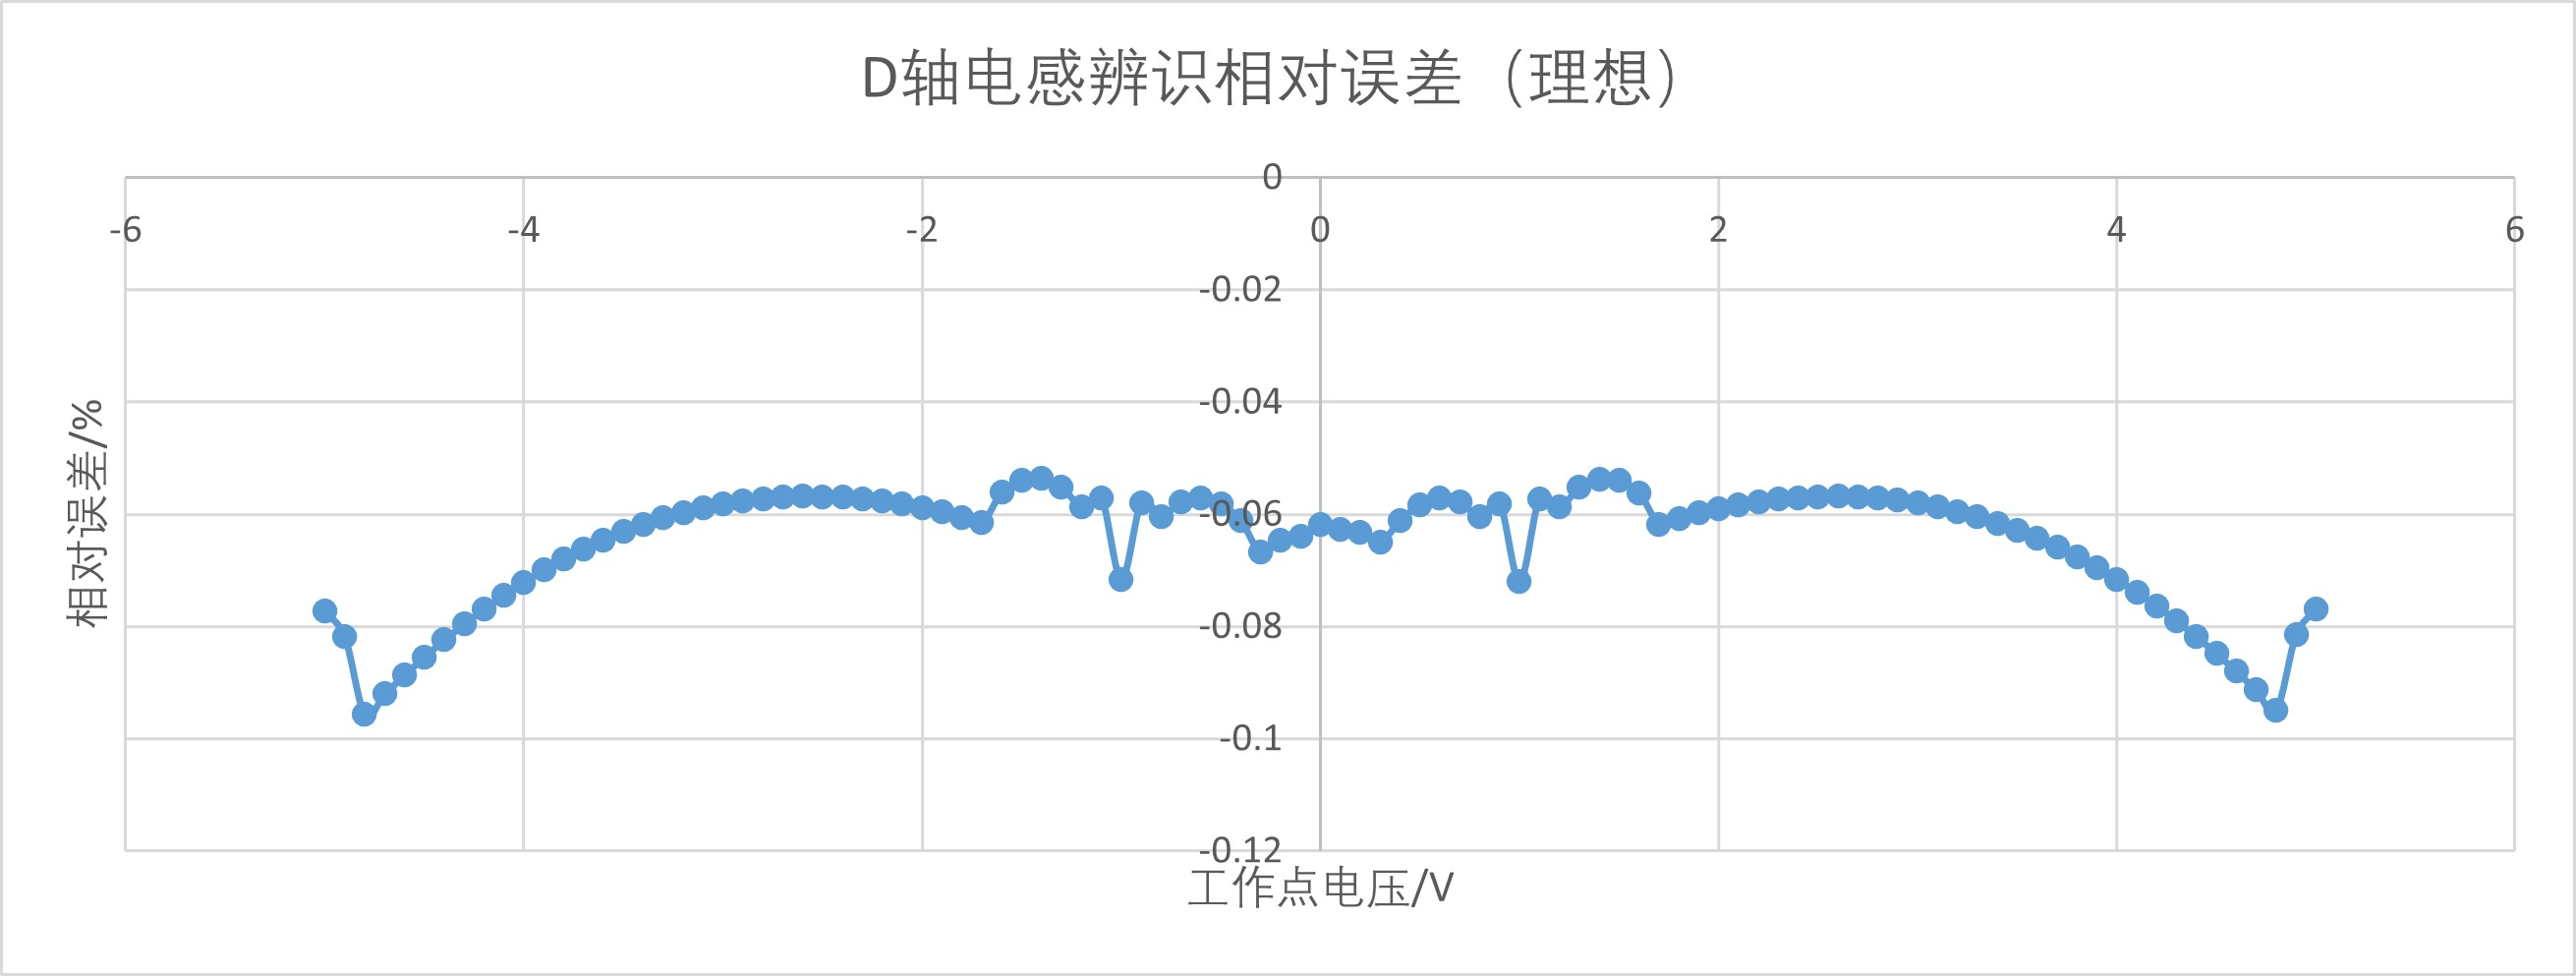
\includegraphics[width=0.8\textwidth]
    {图片/D轴工作点相对误差分析（仿真，理想状态）.jpg}
    \caption{D轴工作点相对误差分析（仿真，理想状态）}
\end{figure}

分析数据可知，在没有时延的仿真环境下，相对误差最大不超过0.07\(\%\)，辨识精度极高。

接下来考虑引入PWM时延、逆变器惯性和采样噪声的非理想情况，进行HK辨识仿真。结果如下：
\begin{figure}[H]
    \begin{minipage}{0.5\textwidth}
        \centering
        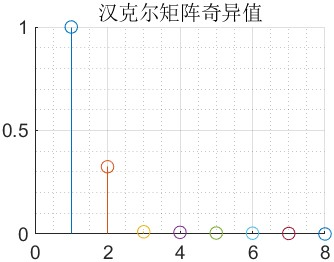
\includegraphics[width=\textwidth]
        {图片/D轴工作点0V归一化奇异值分解图（仿真，非理想状态）.jpg}
        \caption{D轴工作点0V归一化奇异值分解图（仿真，非理想状态）}
    \end{minipage}
    \begin{minipage}{0.5\textwidth}
        \centering
        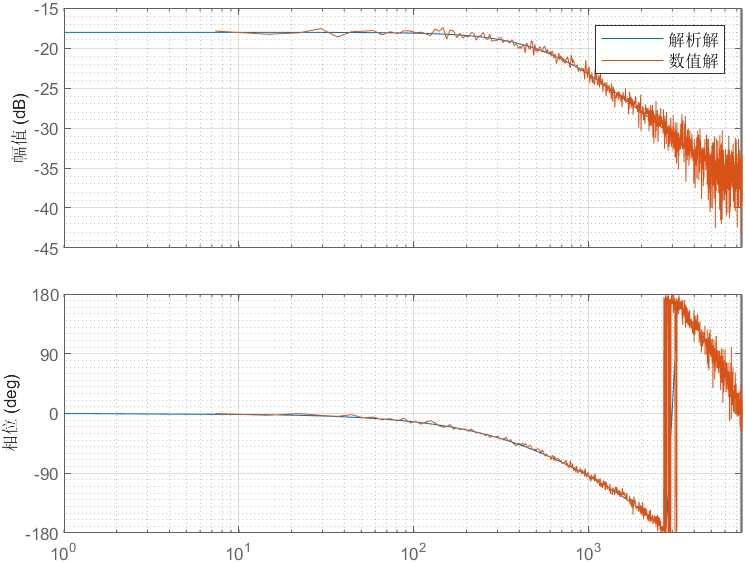
\includegraphics[width=\textwidth]
        {图片/D轴工作点0V解析解与数值解频域对比图（仿真，非理想状态）.jpg}
        \caption{D轴工作点0V解析解与数值解频域对比图（仿真，非理想状态）}
    \end{minipage}
\end{figure}

可以发现，归一化后的奇异值分解显示系统为二阶，这是PWM时延与逆变器惯性导致的结果。辨识传递函数为：
\begin{equation*}
    G_D(z)=\cfrac{-0.0005905 + 0.0006895z^{-1}+0.02919z^{-2}}{1 - 0.7704z^{-1} + 0.004188z^{-2}}
\end{equation*}

数值解与解析解的幅频相关系数为98.91053\(\%\)，相频相关系数为99.81401\(\%\)，拟合优度87.16411\(\%\)
拟合程度相较于无时延有一定的下降（尤其是拟合优度），但整体仍处于较高拟合程度。
解析解极点位于\(z_{pD}=0.7649,0.0055\)处，根据\(L_d=-\cfrac{T_sR_s}{\ln(z_{pD})}\)，选取靠近单位圆的\(z_{pD}=0.7669\)为
电机本身的模态，得到辨识结果\(L_d=1.99010\)mH，相对误差-0.49494\(\%\)，相对误差有所上升。

同样从-5V到5V，以0.1V为步长进行辨识，辨识结果如下图所示：
\begin{figure}[H]
    \centering
    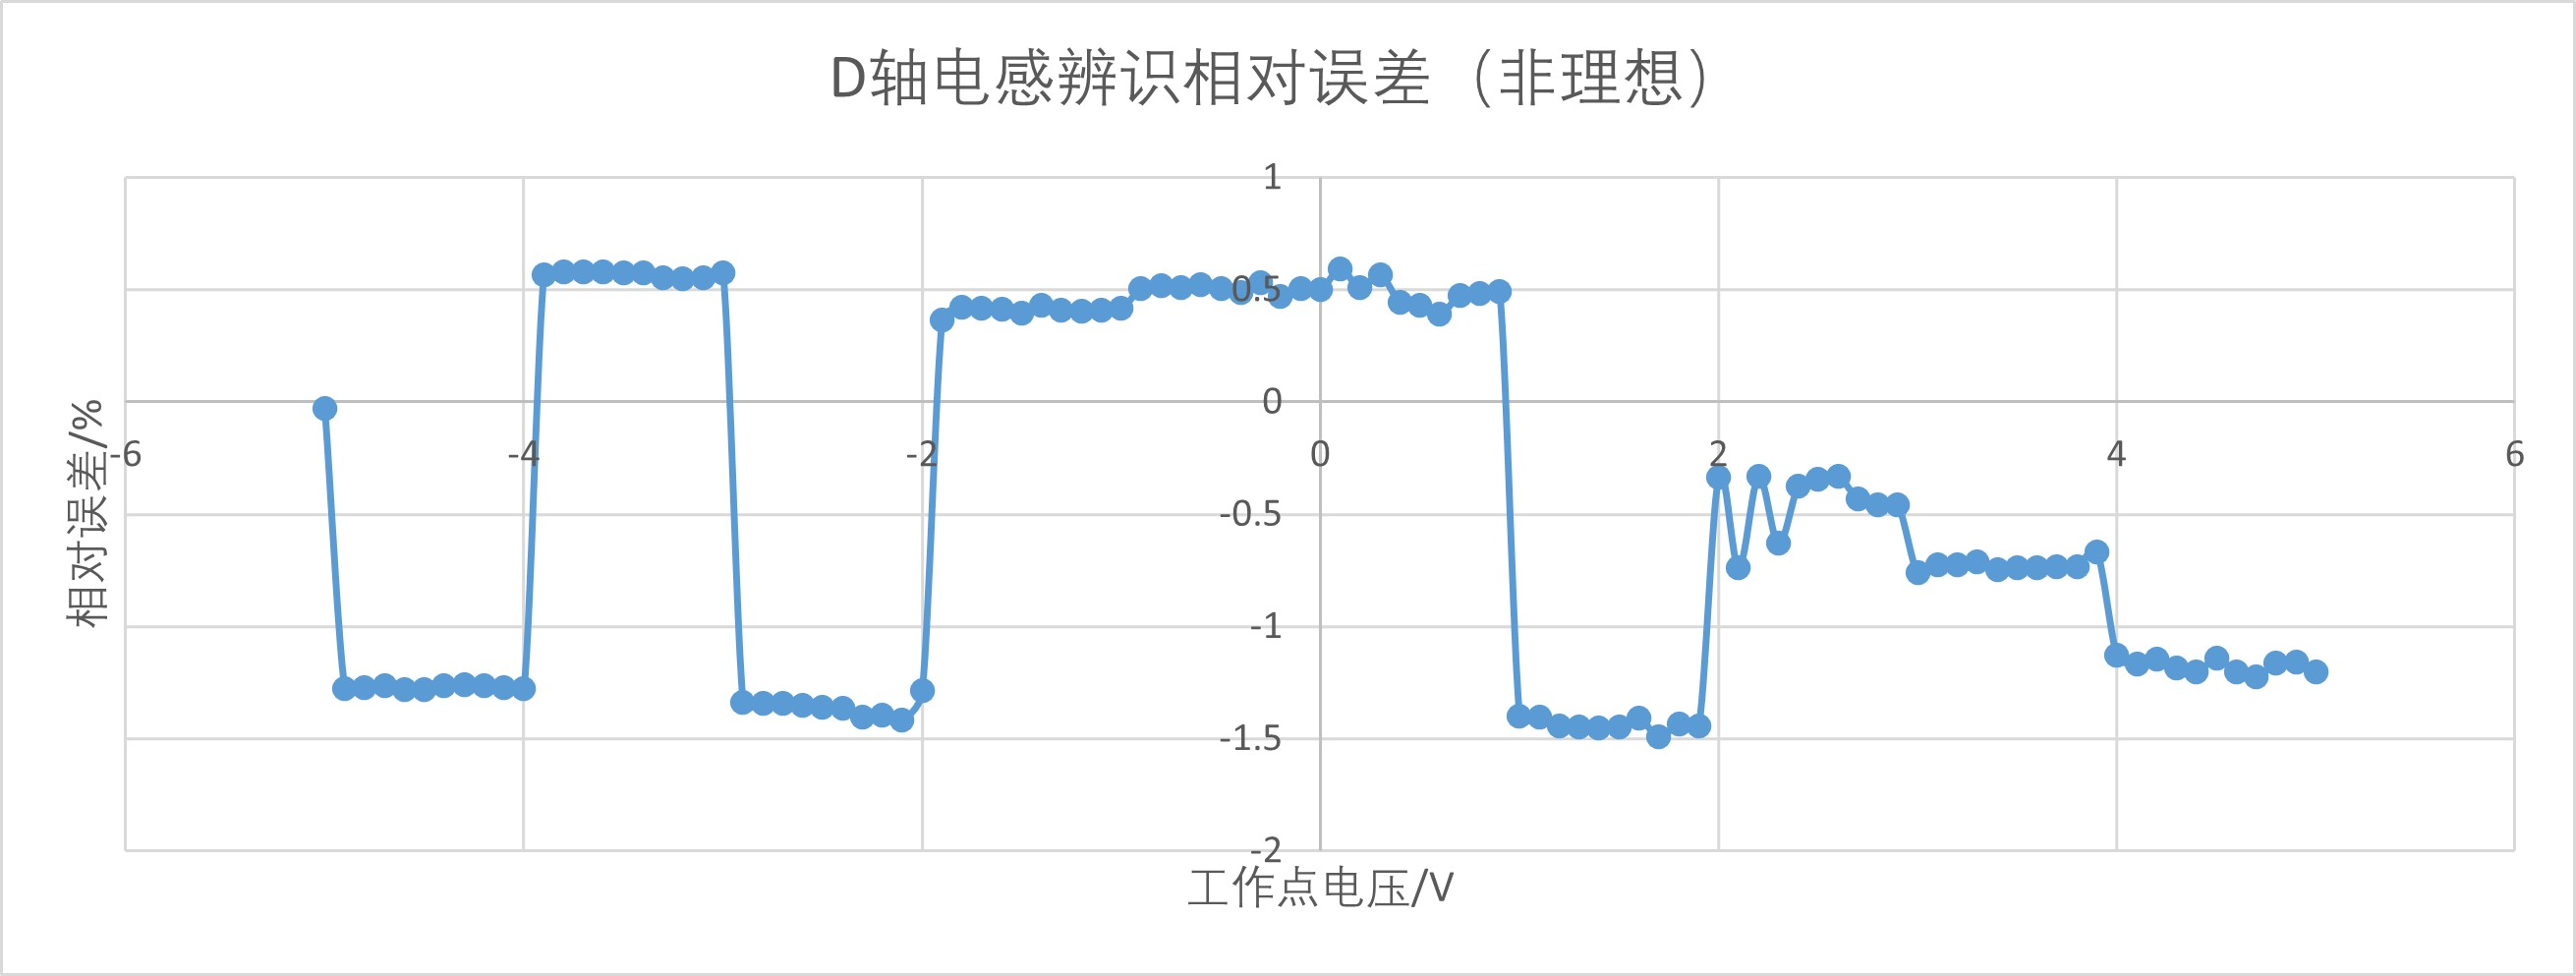
\includegraphics[width=0.8\textwidth]
    {图片/D轴工作点相对误差分析（仿真，非理想状态）.jpg}
    \caption{D轴工作点相对误差分析（仿真，非理想状态）}
\end{figure}

分析数据可知，在含有时延的仿真环境下，相对误差最大超过了3\(\%\)，辨识精度相较于无时延有所下降，但仍处于可接受范围内。分析造成
相对误差增大的原因主要一是PWM时延、逆变器惯性和采样噪声等非理想因素降低了信噪比，影响了辨识精度。

\subsubsection{Q轴同步电感辨识仿真}

根据Q轴电路方程：
\begin{equation*}
    u_q=R_si_q+L_d\cfrac{di_q}{dt}+\omega_e(L_di_d+\psi_m)
\end{equation*}

若要消除交叉耦合，则可以通过电气或机械锁轴使得
\(\omega_e=0\)实现。但实测发现电气锁轴或机械堵转都难以彻底消除微动，交叉耦合项难以完全抵消（详见\ref{sec:电气锁轴方法}
和\ref{sec:机械堵转方法}）。因此最终选择进行数据后处理方法。

根据Q轴电路方程，可以变形得到：
\begin{equation*}
    u_q-\omega_e(L_di_d+\psi_m)=R_si_q+L_q\cfrac{di_q}{dt}
\end{equation*}

因此，通过实时记录某一拍的\(u_q,\omega_e,i_d,i_q\)，结合\(L_d,R_s,\psi_m\)的辨识结果，可以将运动耦合项完全补偿，
得到实际上给定Q轴RL电路的输入信号为\(u_q'=u_q-\omega_e(L_di_d+\psi_m)\)，
此时传递函数为\(G_Q(s)=\cfrac{I_q(s)}{U_q'(s)}=\cfrac{1}{R_s+sL_q}\)（其中永磁体磁链的辨识依赖于稳态模型，不包含复杂的信号处理，
详见\ref{sec:永磁体磁链测量}）。

与D轴类似，首先不考虑PWM和逆变器的时延，在0V工作点附近进行HK辨识，结果如下：
\begin{figure}[H]
    \begin{minipage}{0.5\textwidth}
        \centering
        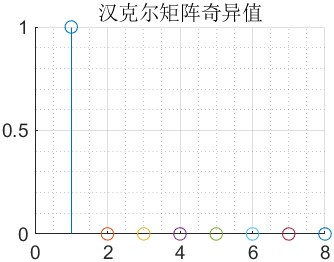
\includegraphics[width=\textwidth]
        {图片/Q轴工作点0V归一化奇异值分解图（仿真，理想状态）.jpg}
        \caption{Q轴工作点0V归一化奇异值分解图（仿真，理想状态）}
    \end{minipage}
    \begin{minipage}{0.5\textwidth}
        \centering
        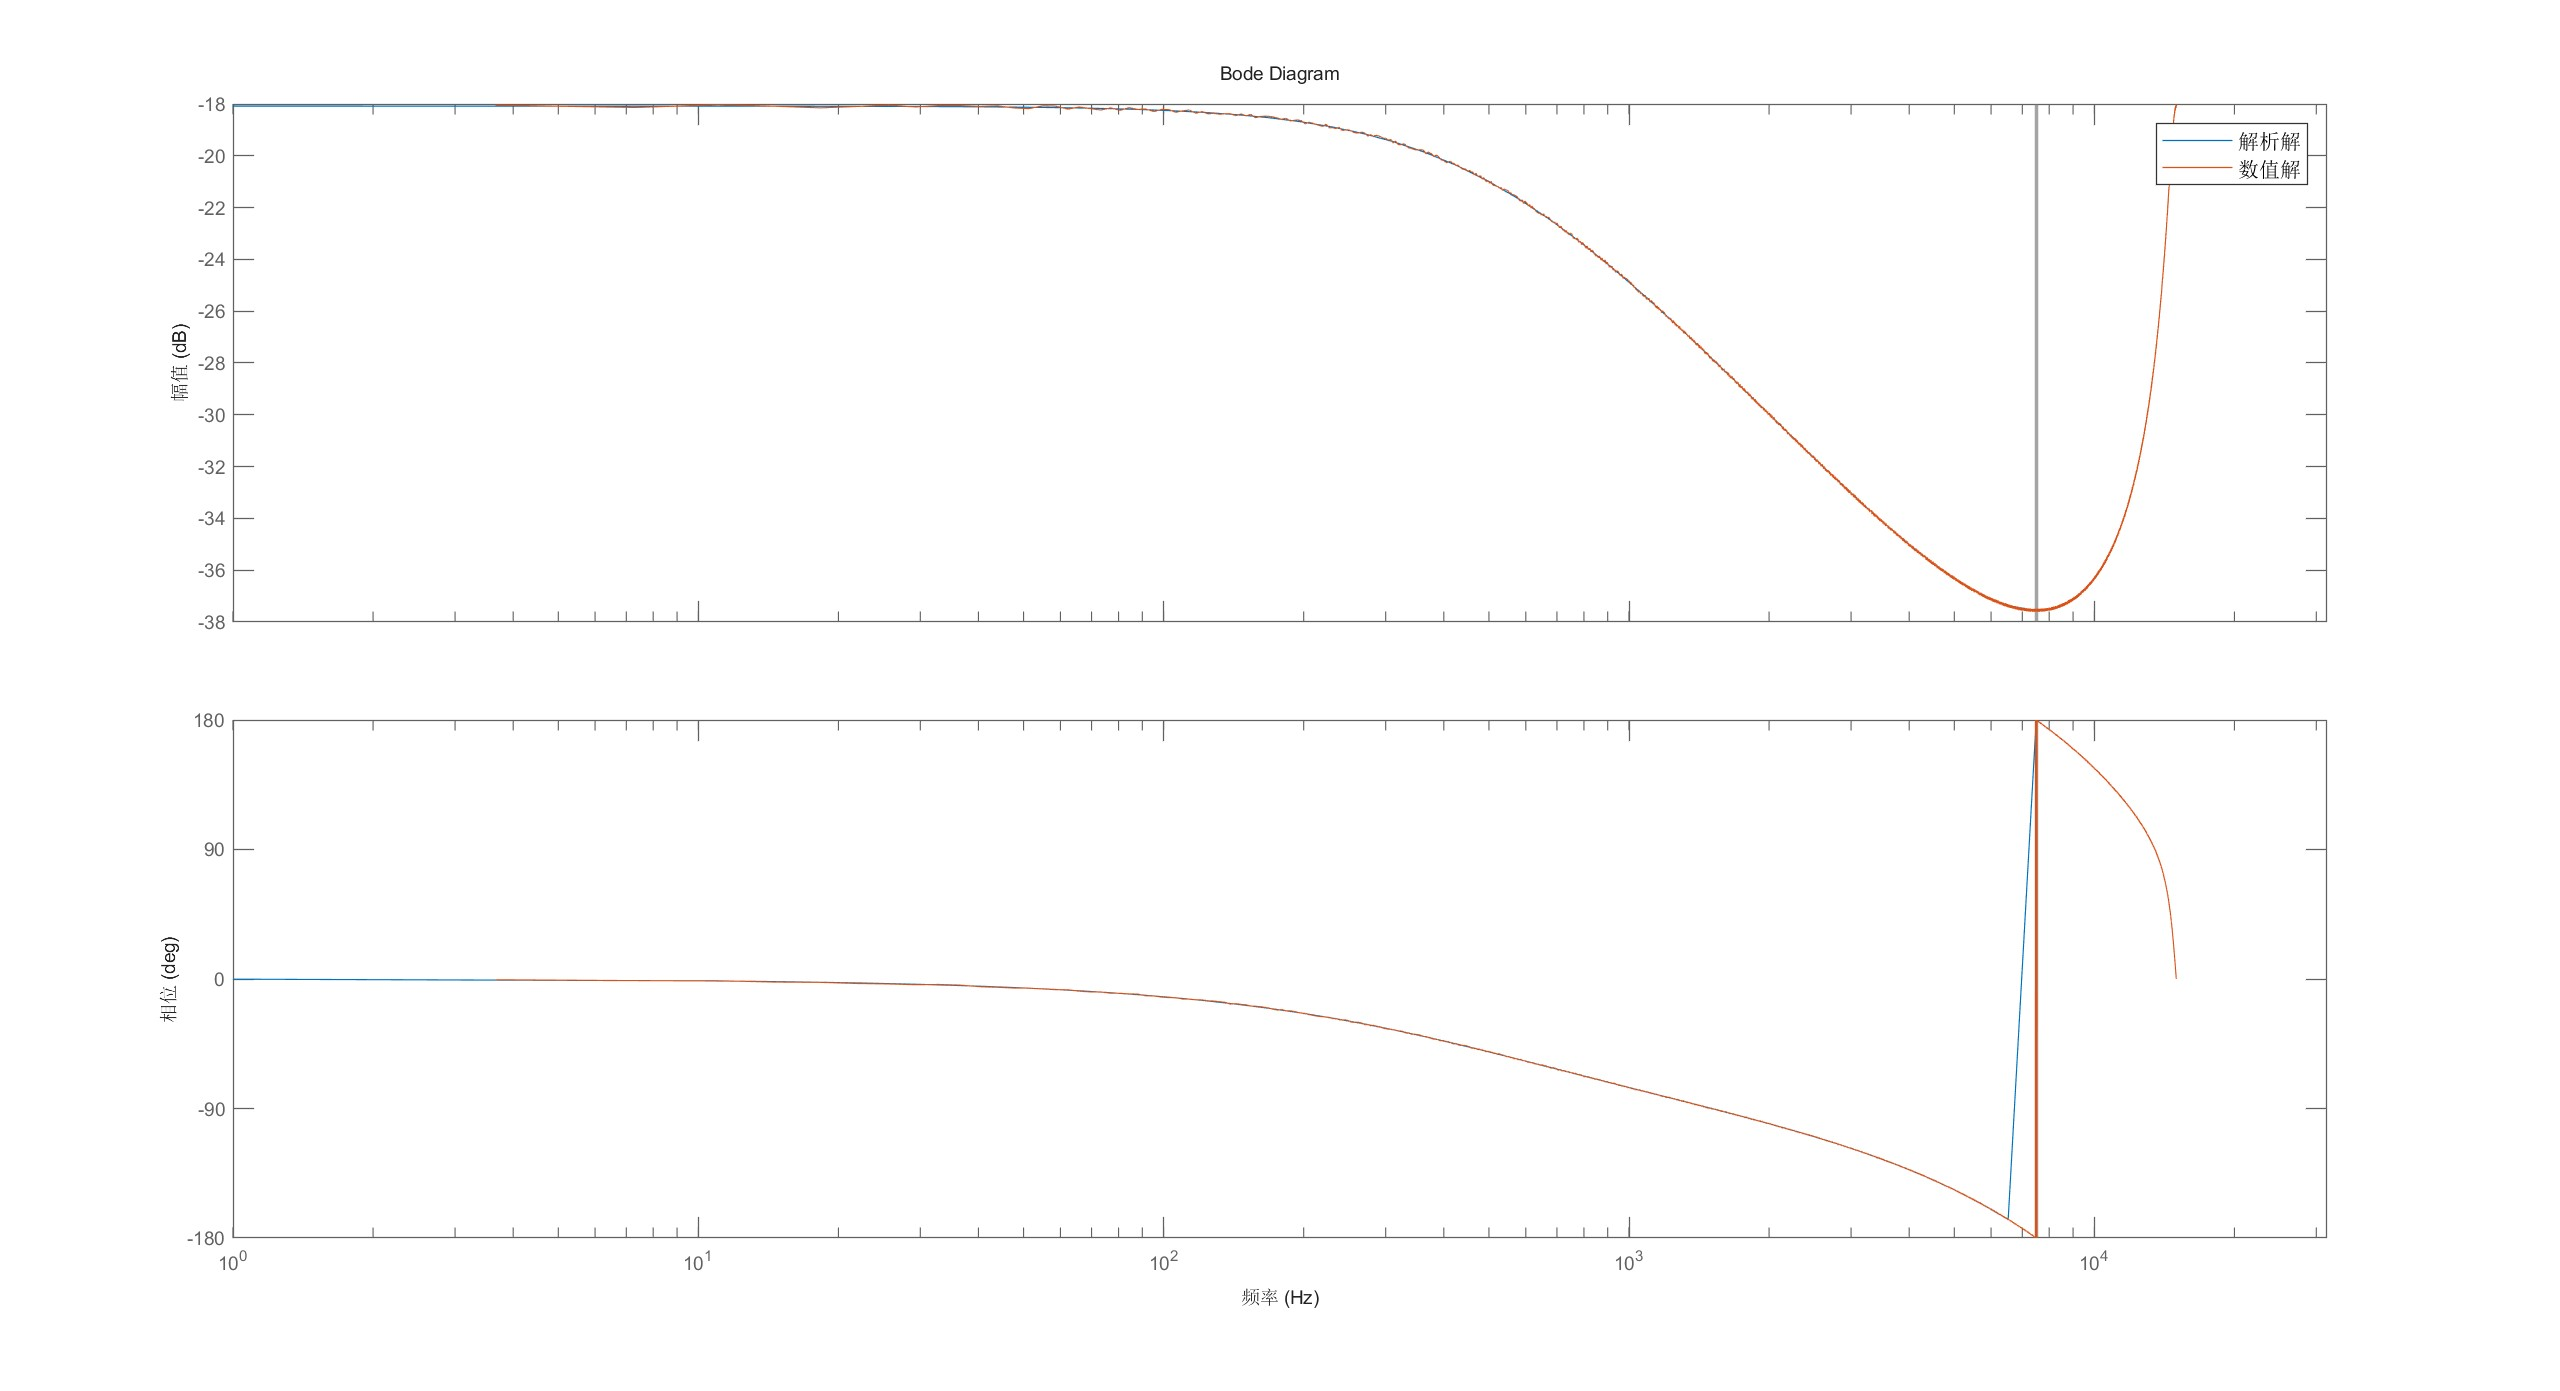
\includegraphics[width=\textwidth]
        {图片/Q轴工作点0V解析解与数值解频域对比图（仿真，理想状态）.jpg}
        \caption{Q轴工作点0V解析解与数值解频域对比图（仿真，理想状态）}
    \end{minipage}
\end{figure}

系统阶次为一阶，辨识传递函数为：
\begin{equation*}
    G_Q(z)=\cfrac{1.834\times 10^{-5} + 0.02396z^{-1}}{1 - 0.8078z^{-1}}
\end{equation*}

数值解与解析解的幅频相关系数为99.96727\(\%\)，相频相关系数为99.99104\(\%\)，
拟合优度97.46235\(\%\)，拟合程度极高。
解析解极点位于\(z_{pQ}=0.8078\)处，根据\(L_q=-\cfrac{T_sR_s}{\ln(z_{pQ})}\)
得到辨识结果\(L_q=2.49837\)mH，相对误差-0.06524\(\%\)。

用同样的方法，从-5V到5V，以0.1V为步长进行辨识，辨识结果如下图所示：
\begin{figure}[H]
    \centering
    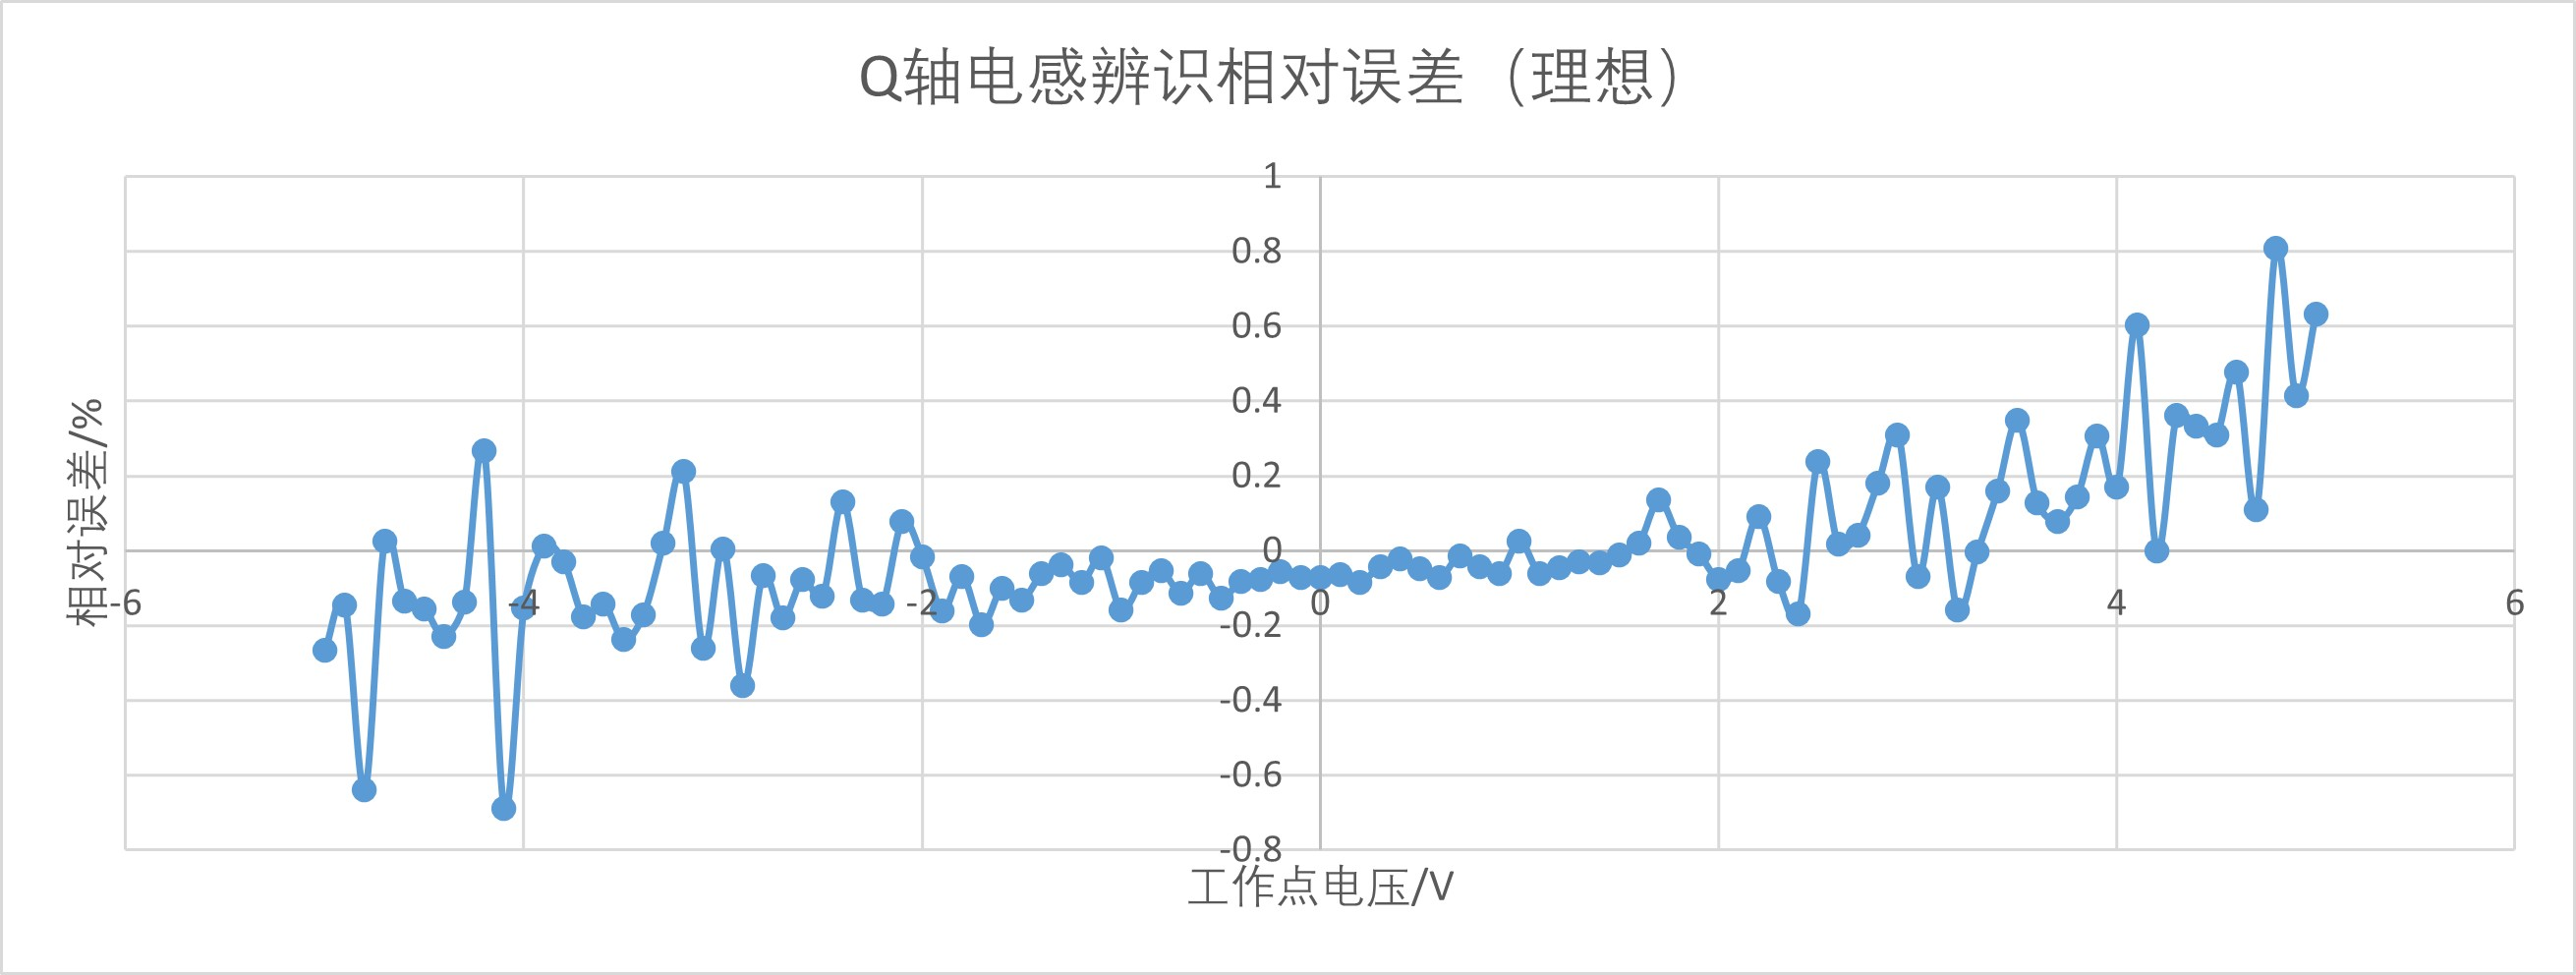
\includegraphics[width=0.8\textwidth]
    {图片/Q轴工作点相对误差分析（仿真，理想状态）.jpg}
    \caption{Q轴工作点相对误差分析（仿真，理想状态）}
\end{figure}

在没有时延的仿真环境下，相对误差最大不超过1\(\%\)，同样具有较高的辨识精度。

接下来在非理想状态下，进行Q轴的HK辨识，在0V工作点附近的辨识结果如下：
\begin{figure}[H]
    \begin{minipage}{0.5\textwidth}
        \centering
        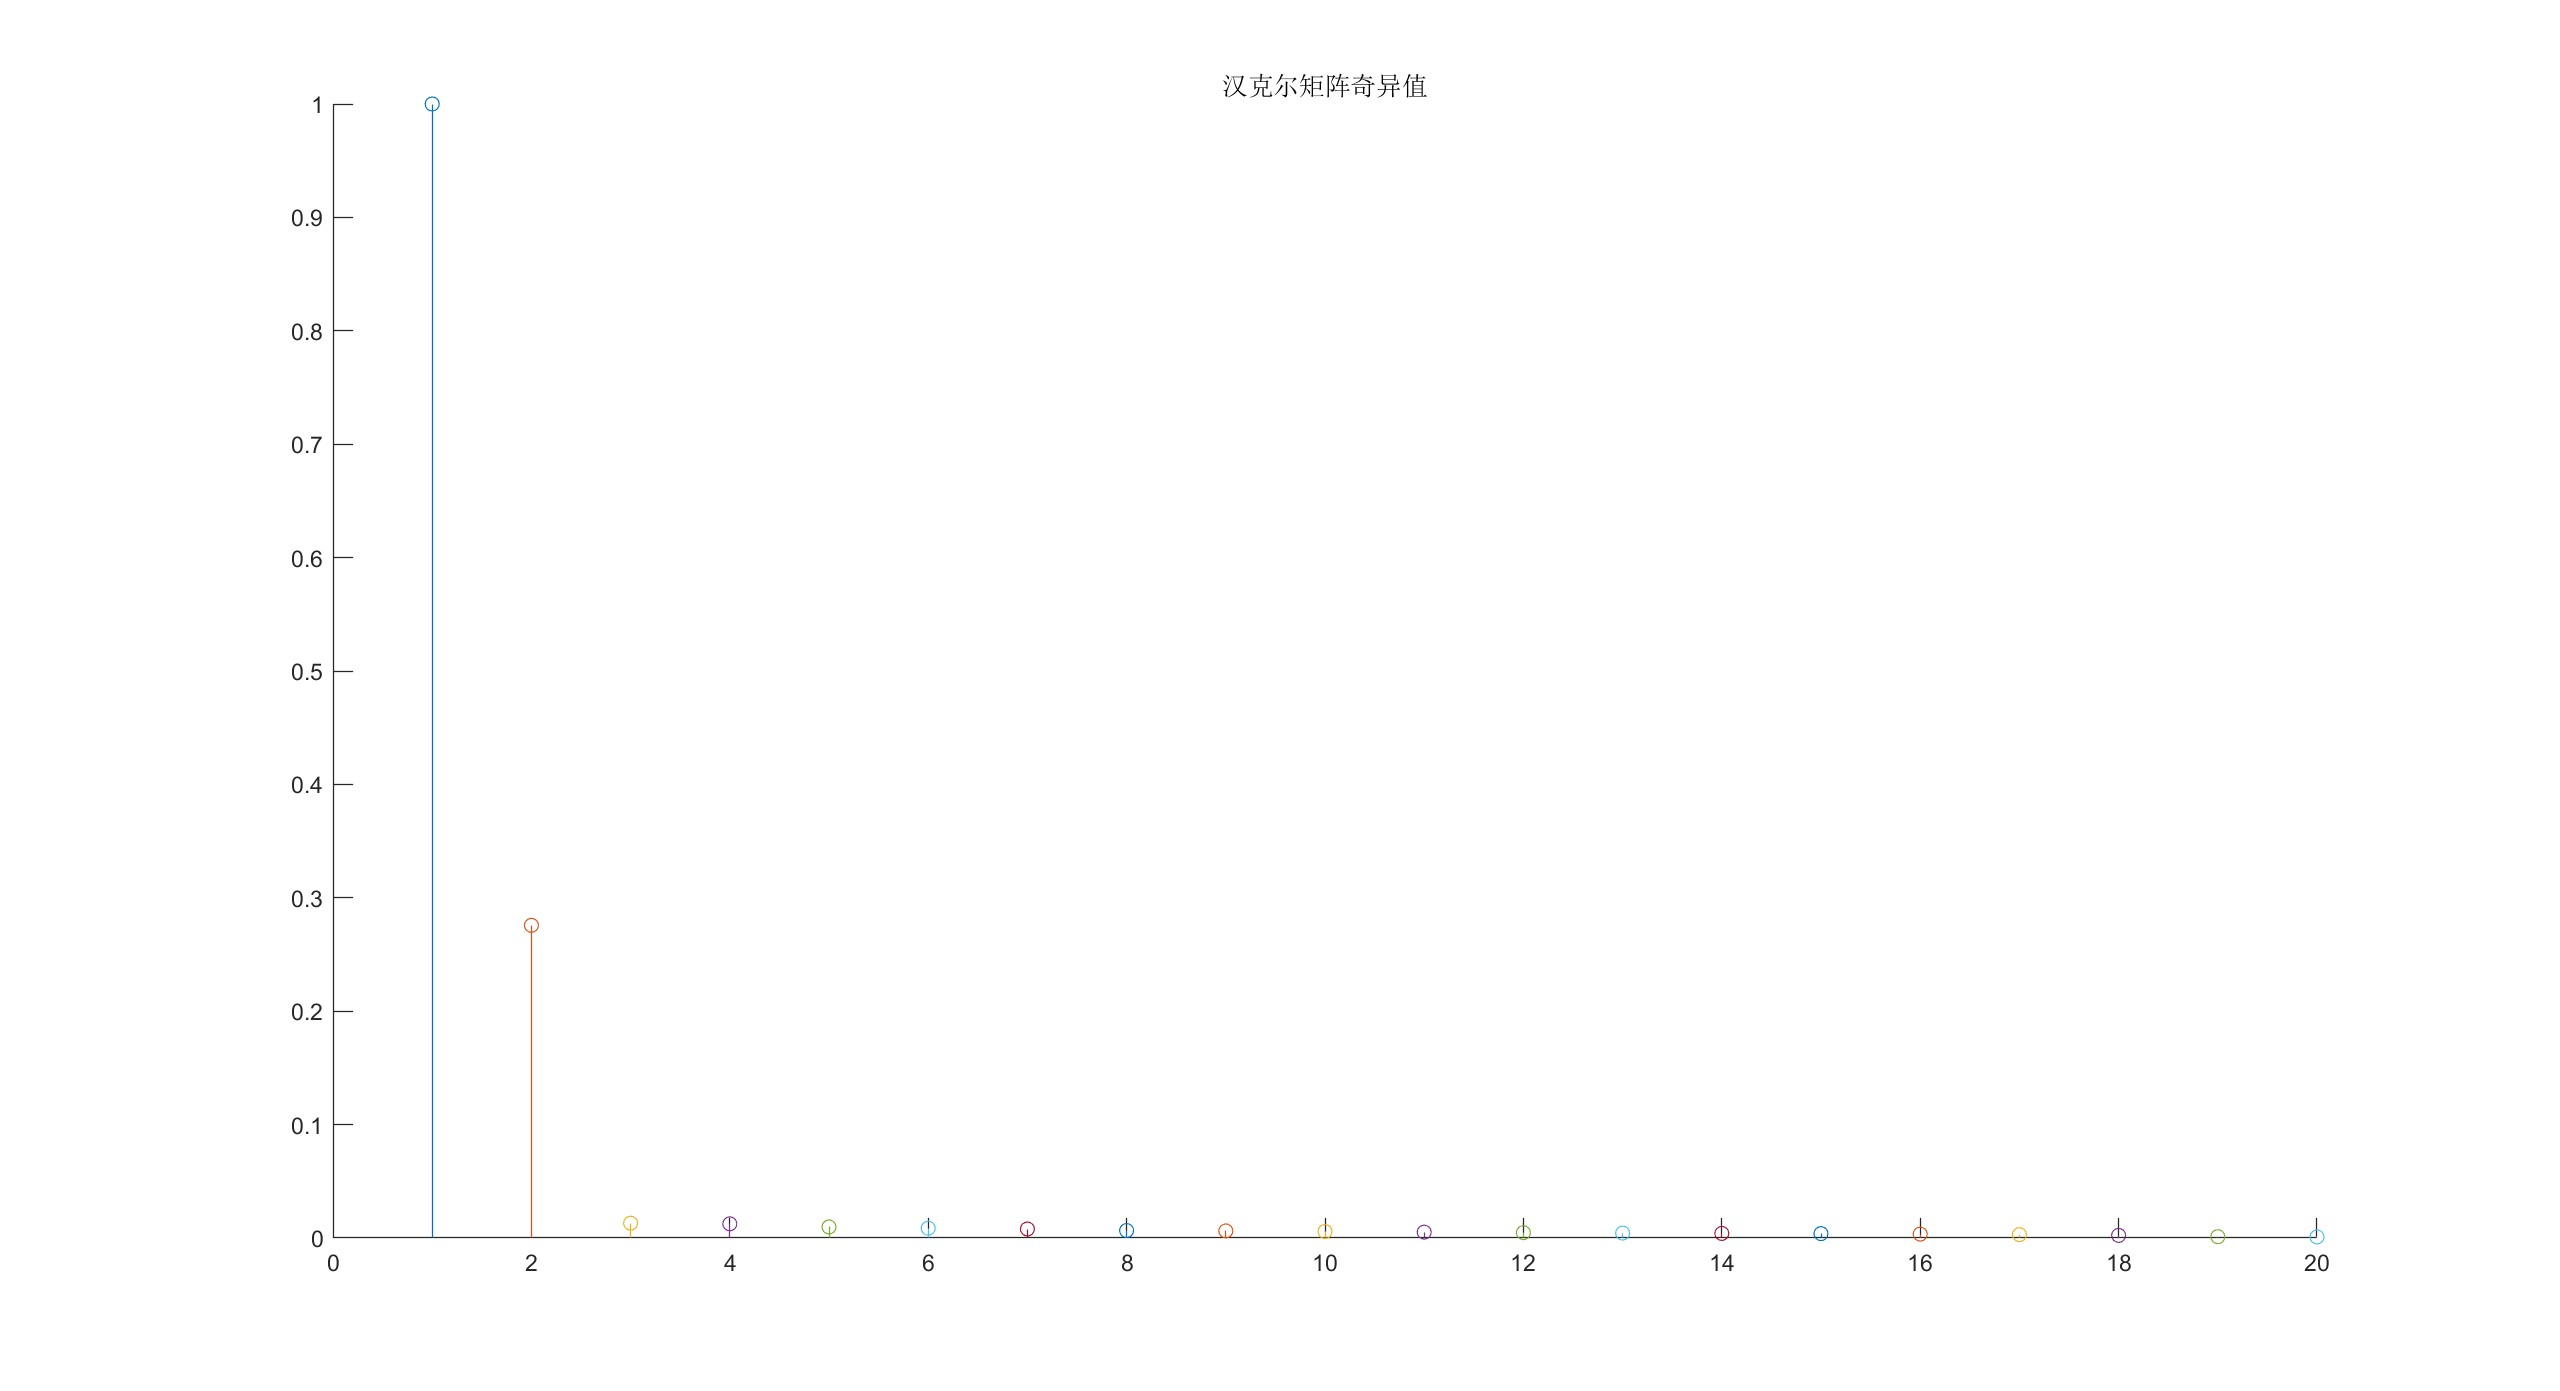
\includegraphics[width=\textwidth]
        {图片/Q轴工作点0V归一化奇异值分解图（仿真，非理想状态）.jpg}
        \caption{Q轴工作点0V归一化奇异值分解图（仿真，非理想状态）}
    \end{minipage}
    \begin{minipage}{0.5\textwidth}
        \centering
        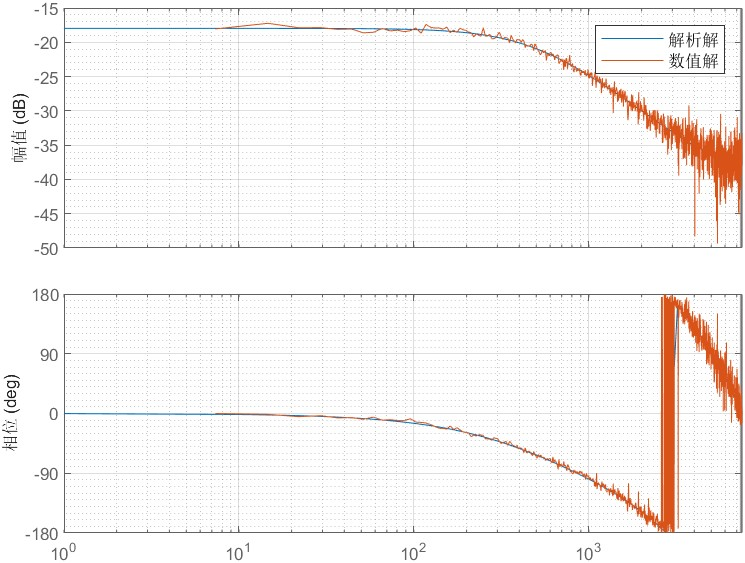
\includegraphics[width=\textwidth]
        {图片/Q轴工作点0V解析解与数值解频域对比图（仿真，非理想状态）.jpg}
        \caption{Q轴工作点0V解析解与数值解频域对比图（仿真，非理想状态）}
    \end{minipage}
\end{figure}

此时由于PWM和逆变器的时延和惯性引入，系统阶次升高到二阶。辨识传递函数为：
\begin{equation*}
    G_Q(z)=\cfrac{-0.0003051 - 0.0001163z^{-1}+0.02413z^{-2}}{1 - 0.8033z^{-1} - 0.007138z^{-2}}
\end{equation*}

数值解与解析解的幅频相关系数为98.98804\(\%\)，相频相关系数为99.74614\(\%\)，
拟合优度86.60122\(\%\)，拟合程度同样降低。
解析解极点位于\(z_{pQ}=0.8092,-0.088\)处，根据\(L_q=-\cfrac{T_sR_s}{\ln(z_{pQ})}\)，选取靠近单位圆的\(z_{pQ}=0.8092\)为
电机本身的模态，得到辨识结果\(L_q=2.51867\)mH，相对误差0.74672\(\%\)，相对误差有所上升。

从-5V到5V，以0.1V为步长进行辨识，辨识结果如下图所示：
\begin{figure}[H]
    \centering
    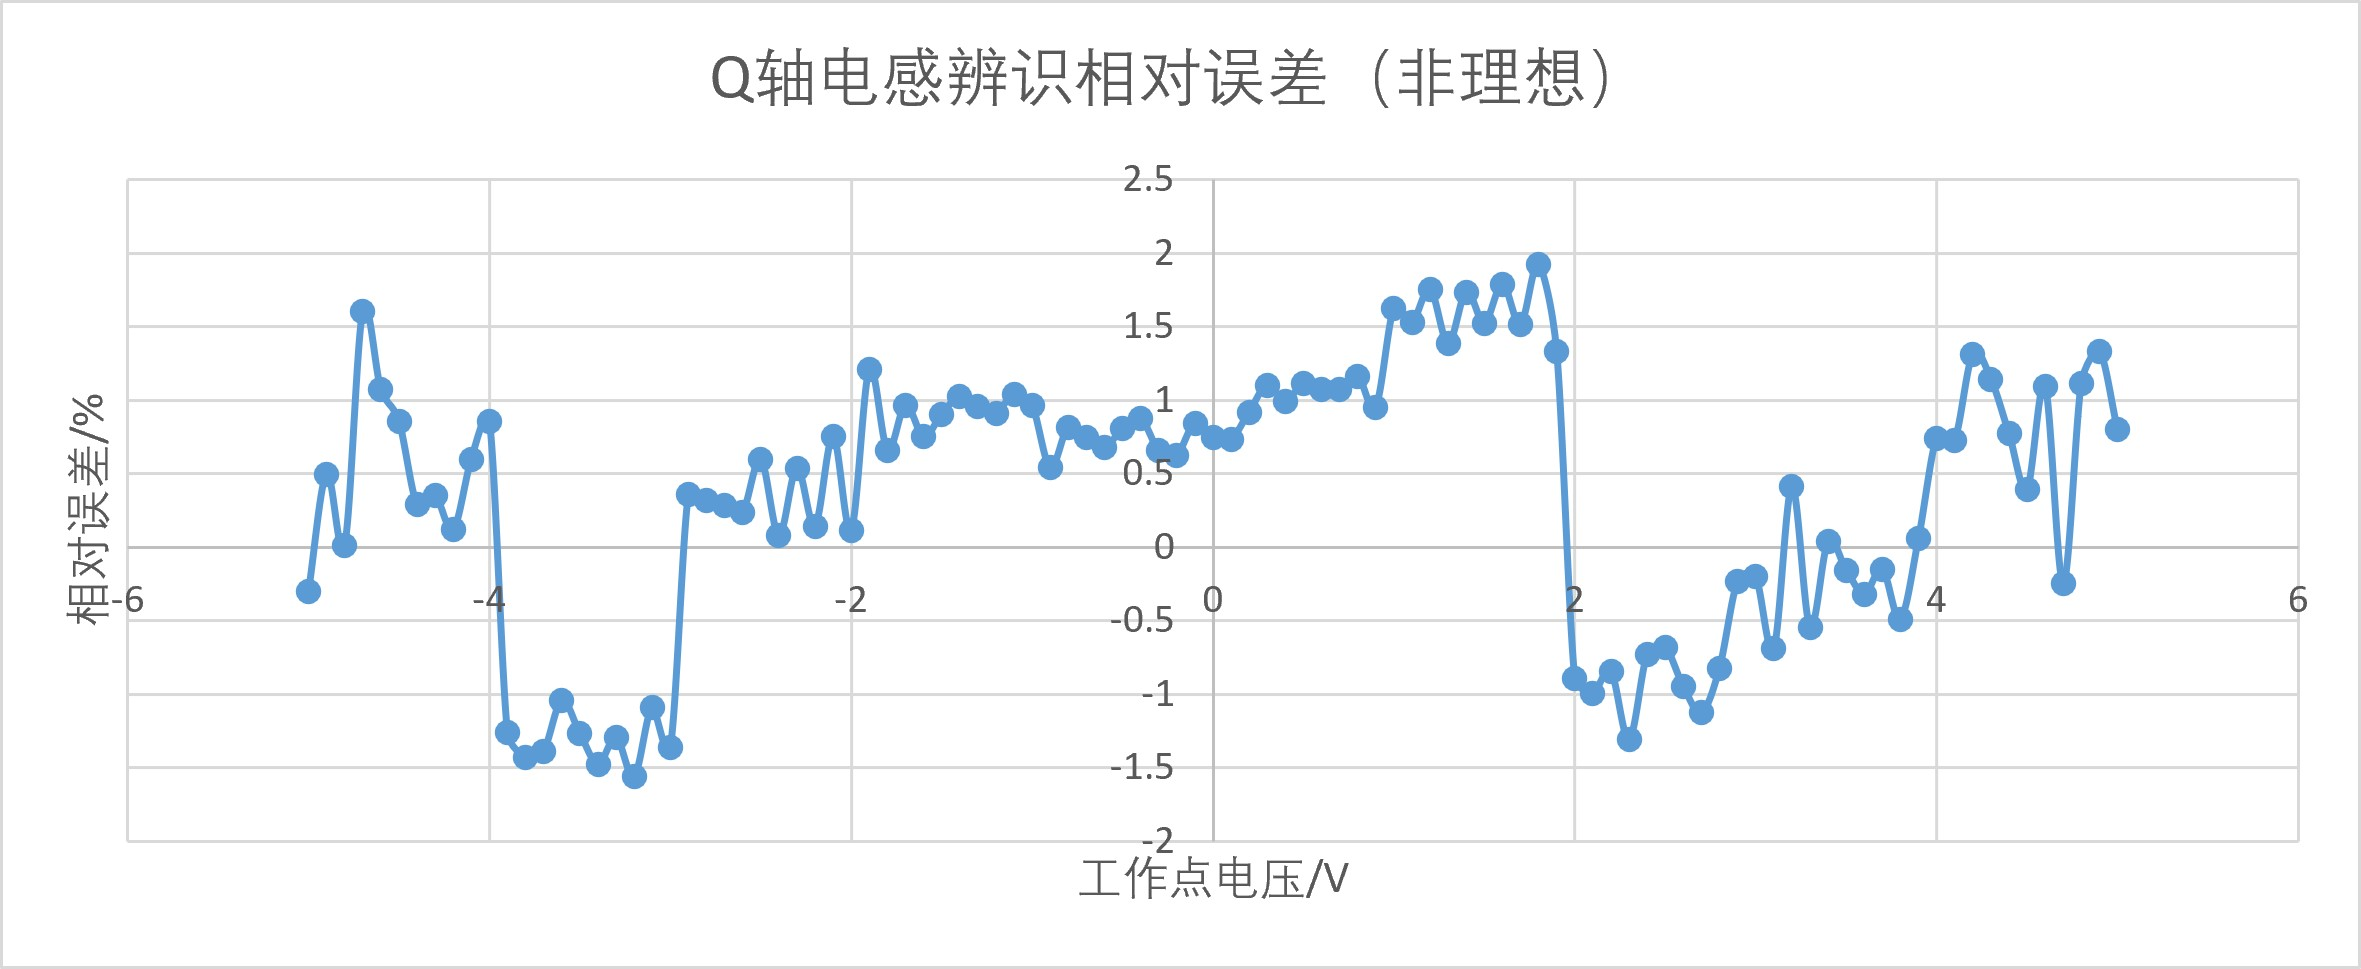
\includegraphics[width=0.8\textwidth]
    {图片/Q轴工作点相对误差分析（仿真，非理想状态）.jpg}
    \caption{Q轴工作点相对误差分析（仿真，非理想状态）}
\end{figure}

在有时延的仿真环境下，辨识精度下降，相对误差升高至2\(\%\)，也在可接受范围内。
相较于D轴，Q轴辨识精度整体较差，分析主要原因就是Q轴的运动解耦并不完全所致。

\subsection{D轴同步电感辨识}

\subsubsection{D轴同步电感辨识过程}

取PWM频率为15kHz，也是电流环控制频率和采样频率。为随机信号级数N=11，伪随机幅值为
1V，在工作点0V、2V、4V、-2V、-4V分别注入伪随机\(u_d\)信号并采集\(i_d\)数据进行分析。

由于串口通信速率有限，这里选择定义输入信号数组\texttt{uint16\(\_\)t m\(\_\)seq[((1 << PRBS\(\_\)N) - 1) * PRBS\(\_\)n];}
和所有需要采集的输出信号数组\texttt{float Output [((1 << PRBS\(\_\)N) - 1) * PRBS\(\_\)n][3];}，在电流控制周期中写入数据，
伪随机信号辨识完成后通过标志位\texttt{bool HK\(\_\)END;}通知速度环控制周期，然后再逐个上传到上位机。

工作点0V，伪随机幅值1V，得到的输入输出曲线、输入自相关函数、输入输出互相关函数、脉冲响应序列如下图所示。
\begin{figure}[H]
    \begin{minipage}{0.5\textwidth}
        \centering
        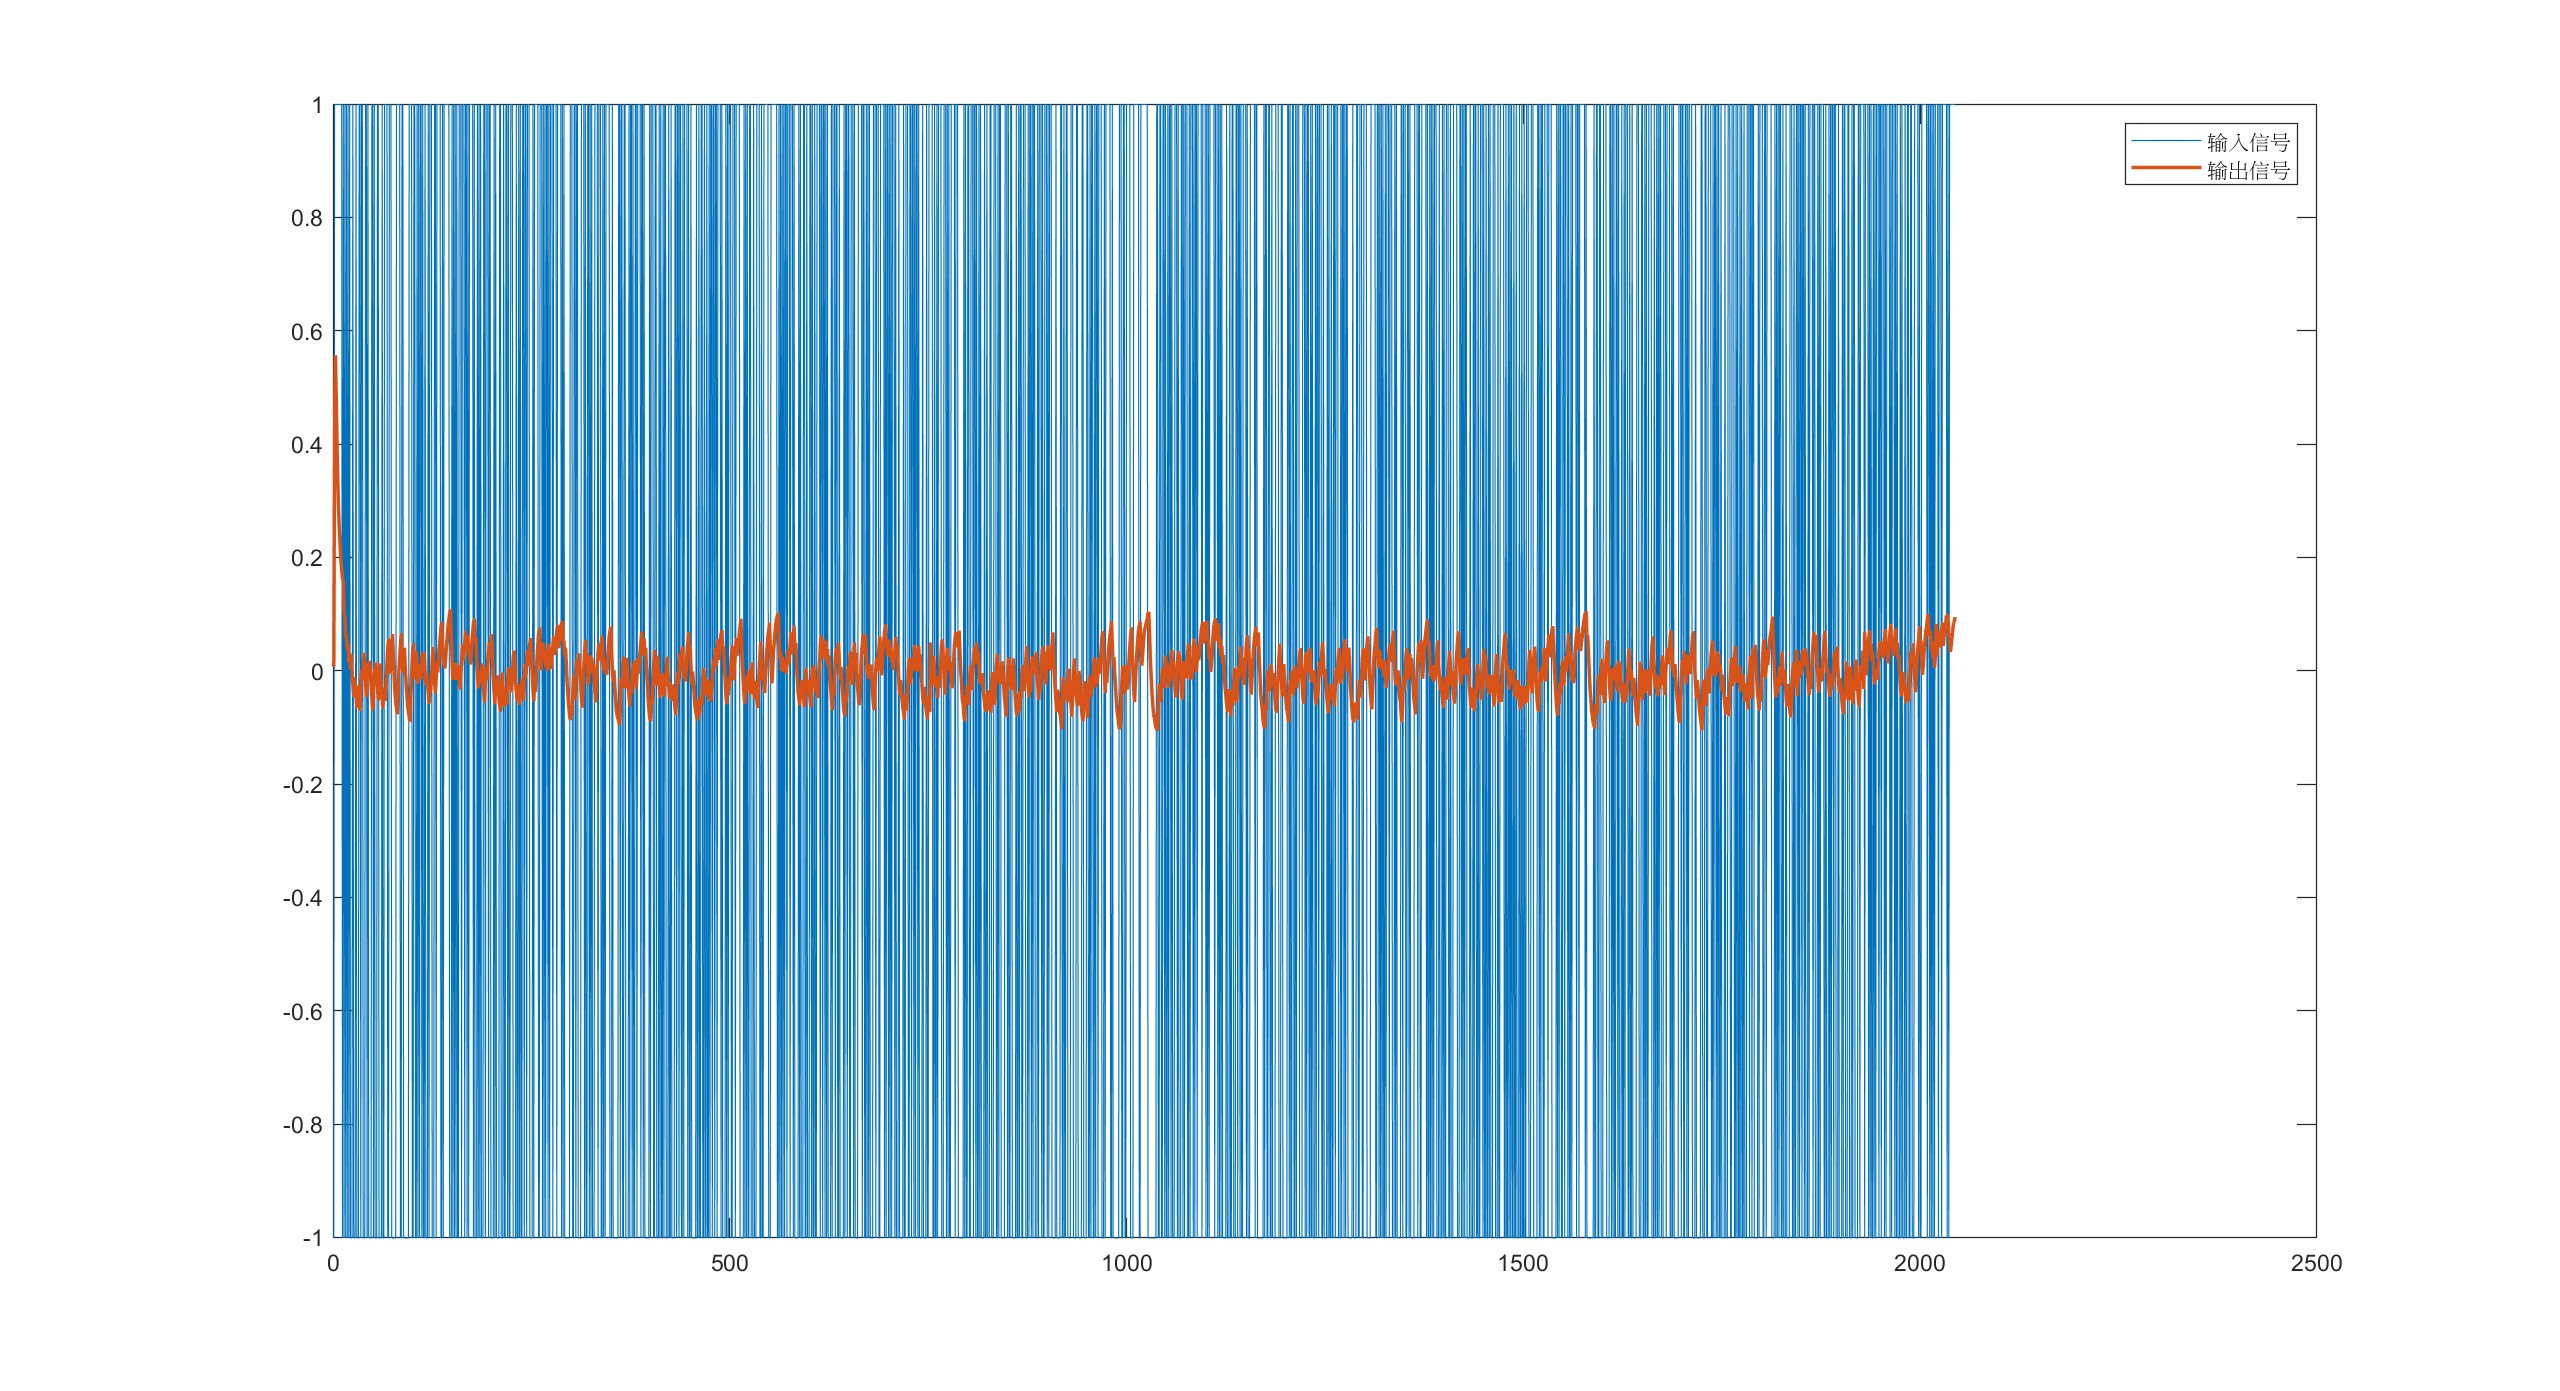
\includegraphics[width=\textwidth]
        {图片/D轴工作点0V输入输出曲线.jpg}
        \caption{D轴工作点0V输入输出曲线}
    \end{minipage}
    \begin{minipage}{0.5\textwidth}
        \centering
        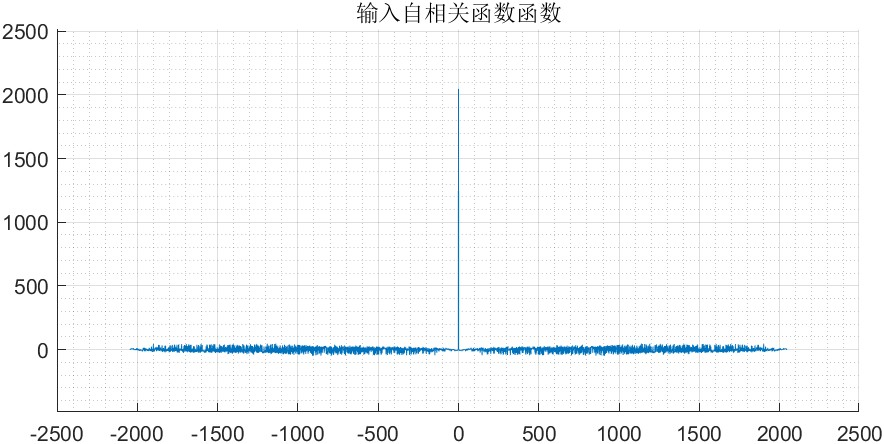
\includegraphics[width=\textwidth]
        {图片/D轴工作点0V输入自相关函数.jpg}
        \caption{D轴工作点0V输入自相关函数}    
    \end{minipage}
\end{figure}
\begin{figure}[H]
    \begin{minipage}{0.5\textwidth}
        \centering
        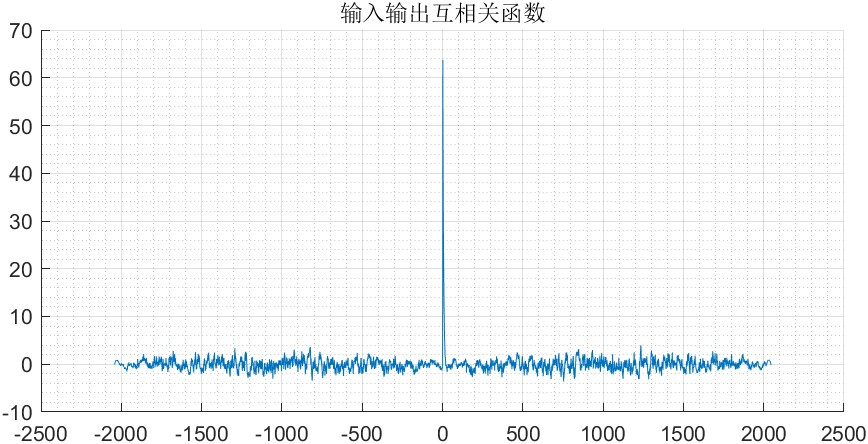
\includegraphics[width=\textwidth]
        {图片/D轴工作点0V输入输出互相关函数.jpg}
        \caption{D轴工作点0V输入输出互相关函数}
    \end{minipage}
    \begin{minipage}{0.5\textwidth}
        \centering
        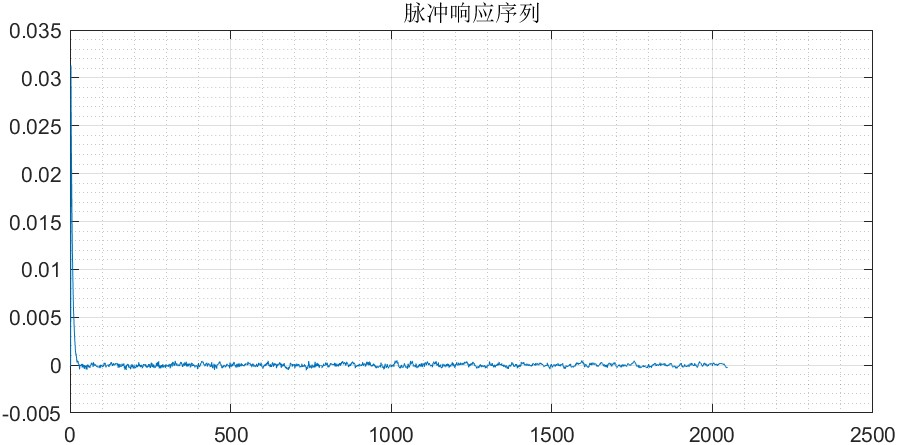
\includegraphics[width=\textwidth]
        {图片/D轴工作点0V脉冲响应序列.jpg}
        \caption{D轴工作点0V脉冲响应序列}
    \end{minipage}
\end{figure}

根据脉冲响应序列，其经过约16个采样周期后暂态响应结束，因此取Hankel矩阵阶次为8。
对Hankel矩阵进行归一化奇异值分解结果如下图所示。
\begin{figure}[H]
    \centering
    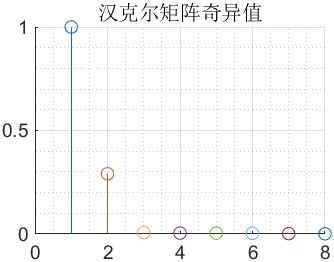
\includegraphics[width=0.8\textwidth]
    {图片/D轴工作点0V奇异值分解图.jpg}
    \caption{D轴工作点0V奇异值分解图}
\end{figure}

奇异值在第三个处发生跳变，因此取系统阶次为2，得到数值频域解和解析频域解如下图所示。
\begin{figure}[H]
    \centering
    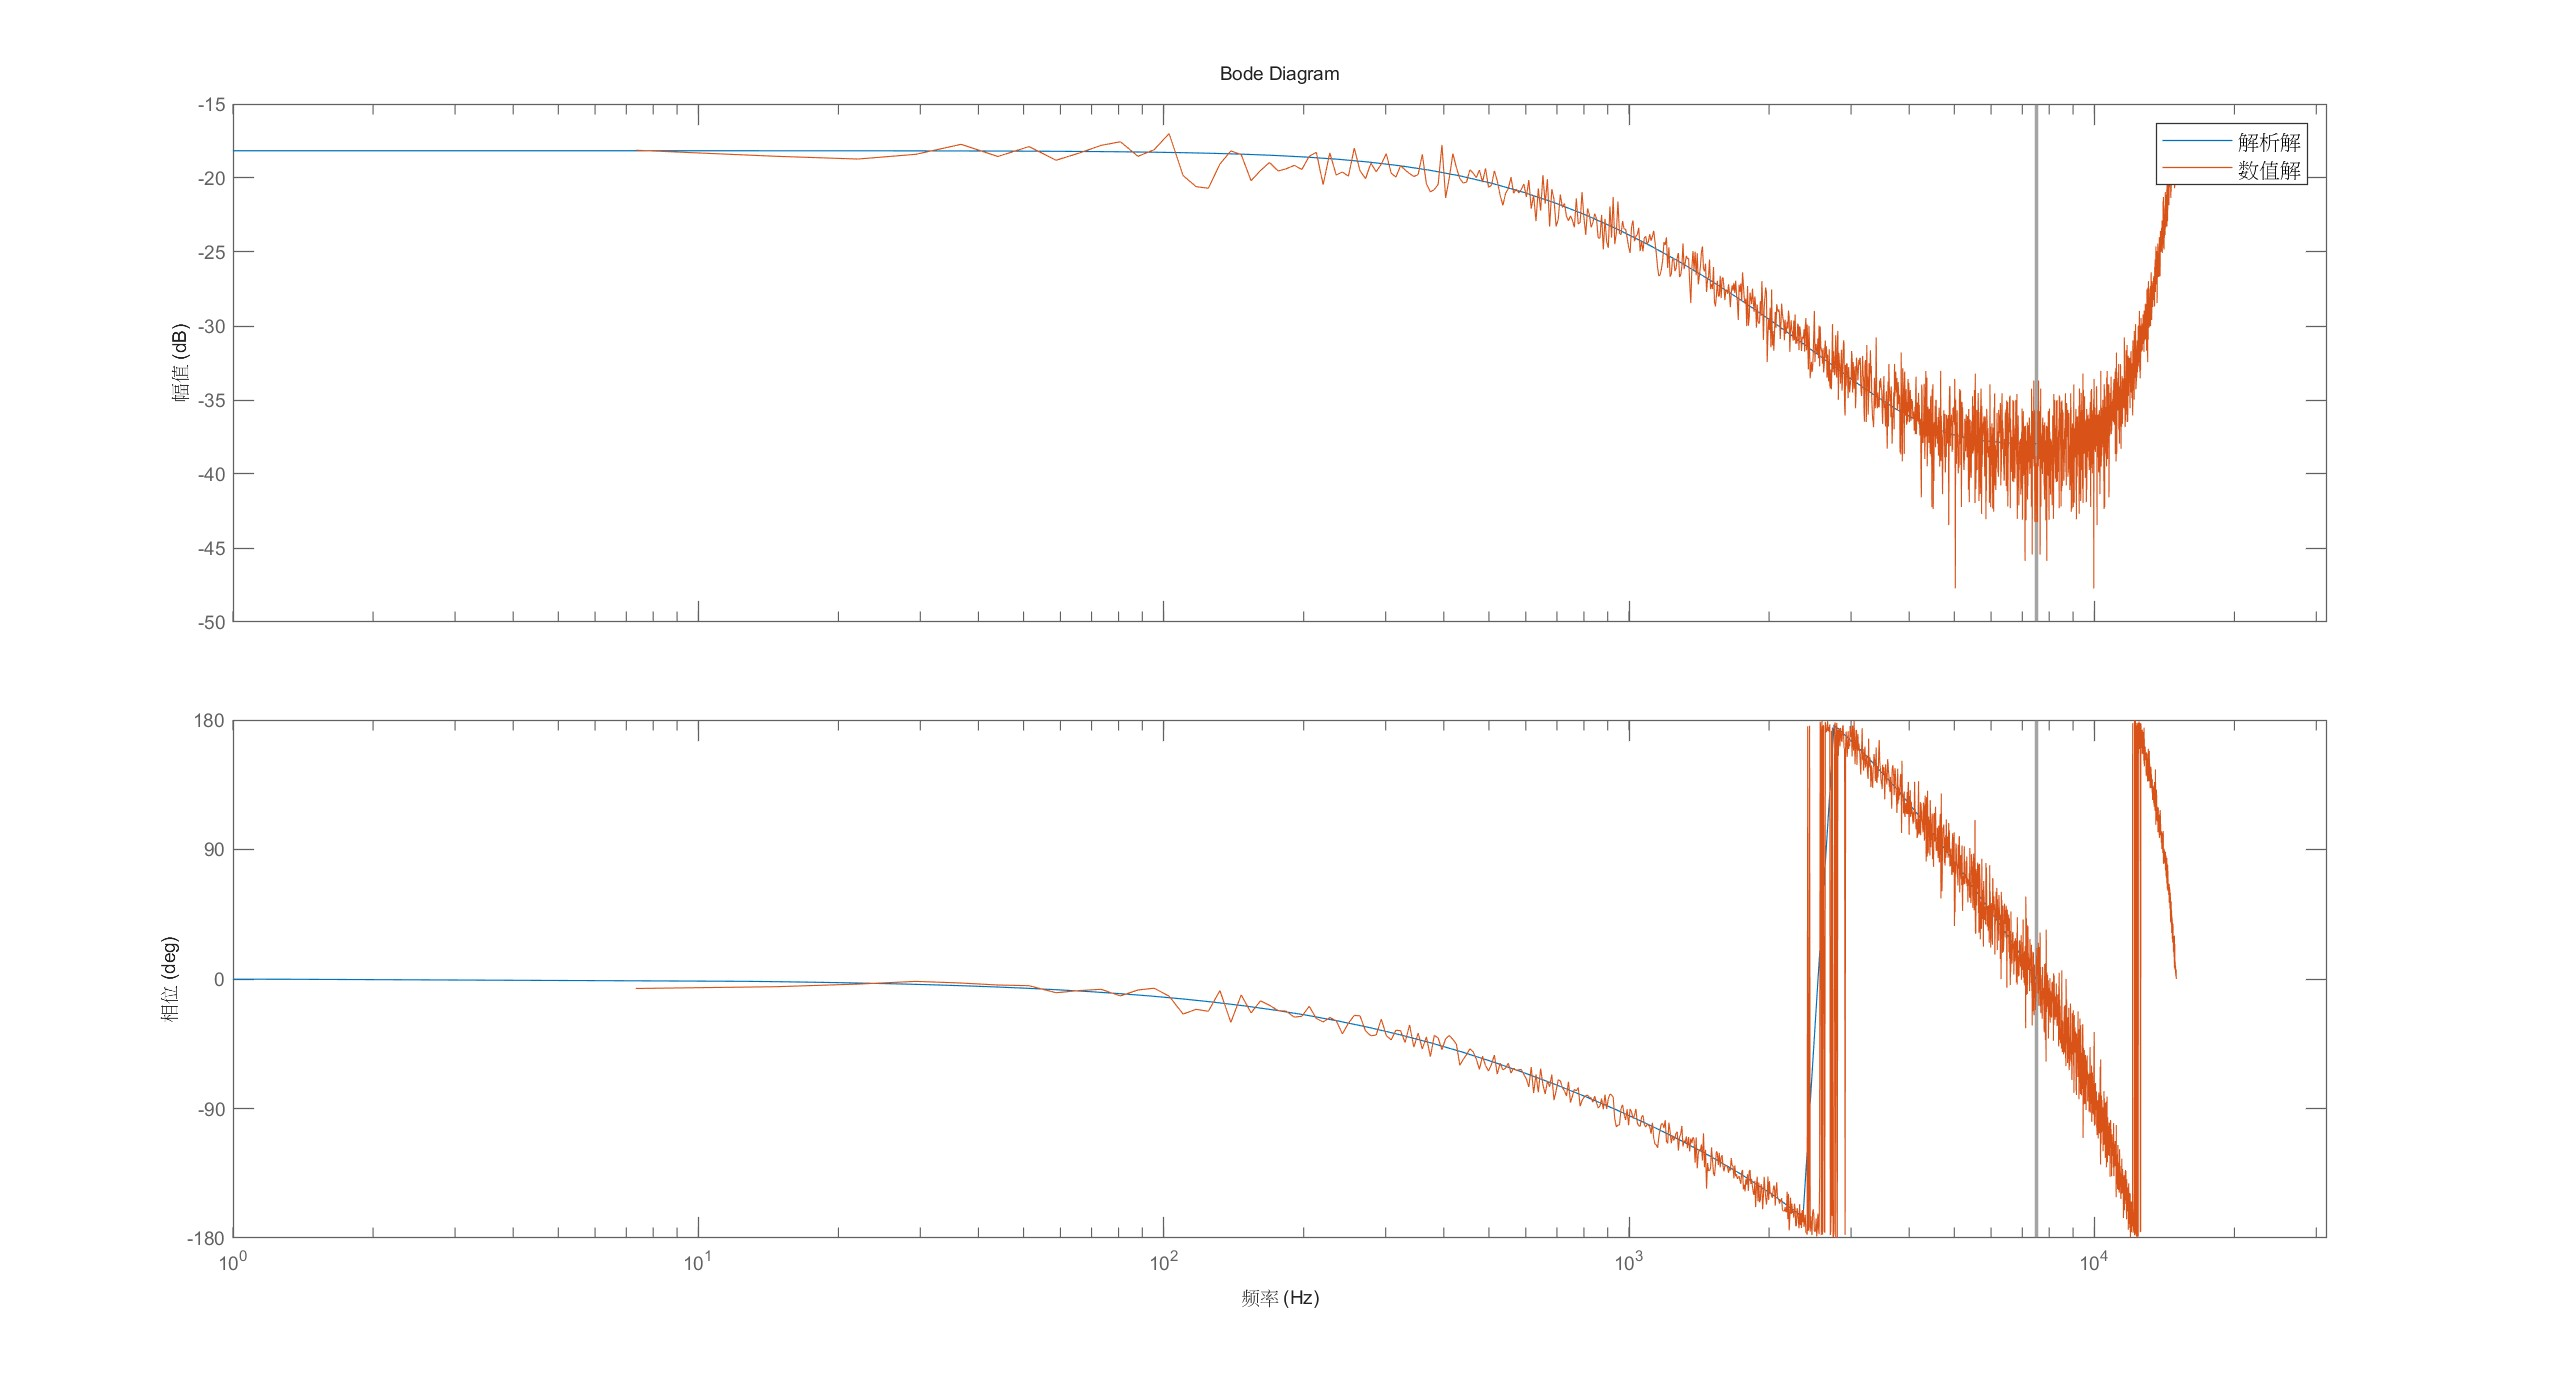
\includegraphics[width=0.8\textwidth]
    {图片/D轴工作点0V数值解和解析解对比.jpg}
    \caption{D轴工作点0V数值解和解析解对比}
\end{figure}

解析解与数值解幅频相关系数为98.89805\(\%\)，
相频相关系数为99.90722\(\%\)，拟合优度86.40194\(\%\)。整体处于较高水平。传递函数为
\(G(z)=\cfrac{-0.0001204  - 0.00006515 z^{-1} + 0.03132z^{-2}}{1 - 0.7754 z^{-1} - 0.03261z^{-2}}\)，两个极点为
0.8154和-0.04。从两个极点中分离出0.8154极点为PWM模态，而-0.04为D轴电路模态。
D轴同步电感可以计算为\(L_d=-\cfrac{R_sT_s}{\ln(z_p)}\)，
可得在0V工作点下D轴同步电感为\(L_d=1.86152\textrm{mH}\)。

后续工作点的辨识过程与上述类似，均采用Hankel矩阵阶次8，系统阶次2，选取幅值较大的极点为电路模态，
利用\(L_d=-\cfrac{R_sT_s}{\ln(z_p)}\)计算D轴电感，不再详述，仅列出较为重要的内容。

工作点2V时，得到的Hankel矩阵奇异值分解和频域响应对比如下图所示。
数值解与解析解的幅频相关系数为98.94669\(\%\)，
相频相关系数为99.94114\(\%\)，拟合优度87.09381\(\%\)。解析解传递函数为
\(G(z)=\cfrac{-0.0001405  + 0.0001453 z^{-1} + 0.03478z^{-2}}{1 - 0.765 z^{-1} - 0.03653z^{-2}}\)，两个极点为
0.8101和-0.0451。得到2V工作点下D轴同步电感为\(L_d=1.80467\textrm{mH}\)。
\begin{figure}[H]
    \begin{minipage}{0.5\textwidth}
        \centering
        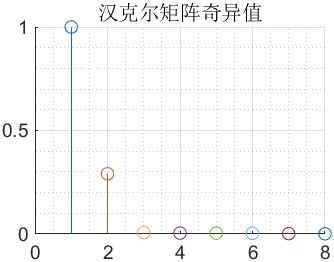
\includegraphics[width=\textwidth]
        {图片/D轴工作点2V奇异值分解图.jpg}
        \caption{D轴工作点2V奇异值分解图}
    \end{minipage}
    \begin{minipage}{0.5\textwidth}
        \centering
        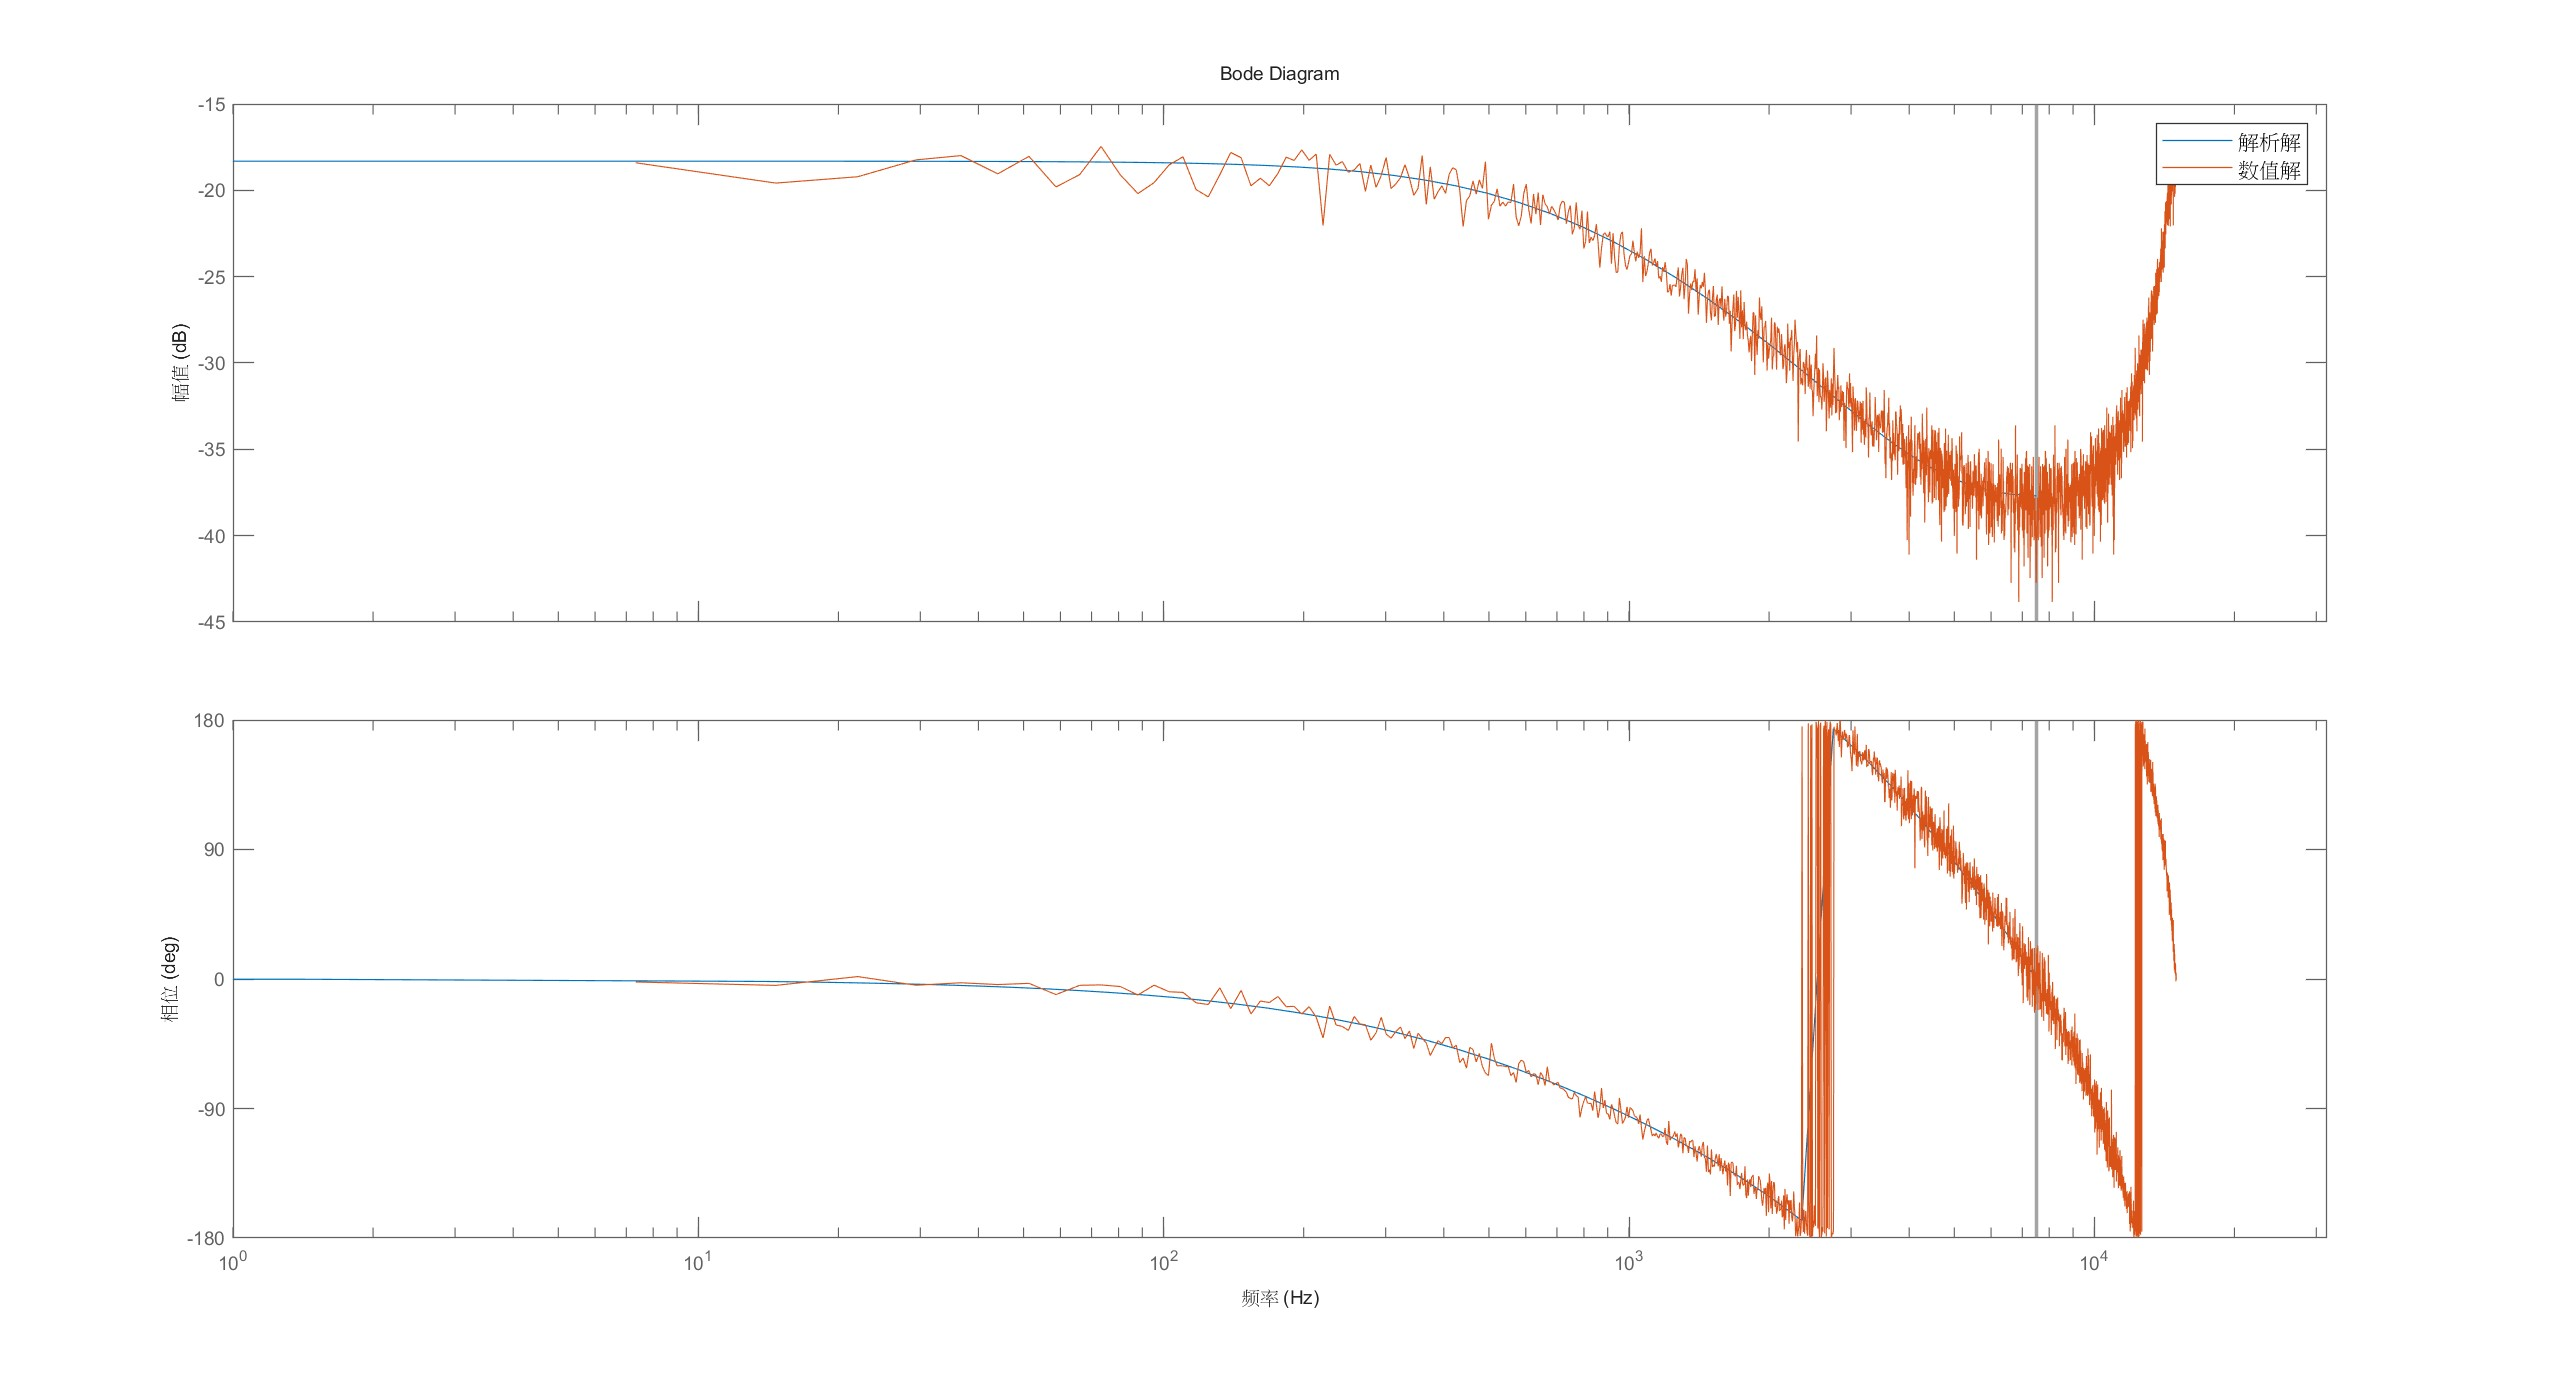
\includegraphics[width=\textwidth]
        {图片/D轴工作点2V数值解和解析解对比.jpg}
        \caption{D轴工作点2V数值解和解析解对比}
    \end{minipage}
\end{figure}

工作点4V时，得到的Hankel矩阵奇异值分解和频域响应对比如下图所示。
数值解与解析解的幅频相关系数为98.97066\(\%\)，
相频相关系数为99.91828\(\%\)，拟合优度86.93735\(\%\)。解析解传递函数为
\(G(z)=\cfrac{0.00005837  - 0.000171 z^{-1} + 0.034z^{-2}}{1 - 0.8461 z^{-1} + 0.0422z^{-2}}\)，两个极点为
0.7929和0.0532。得到4V工作点下D轴同步电感为\(L_d=1.63713\textrm{mH}\)。
\begin{figure}[H]
    \begin{minipage}{0.5\textwidth}
        \centering
        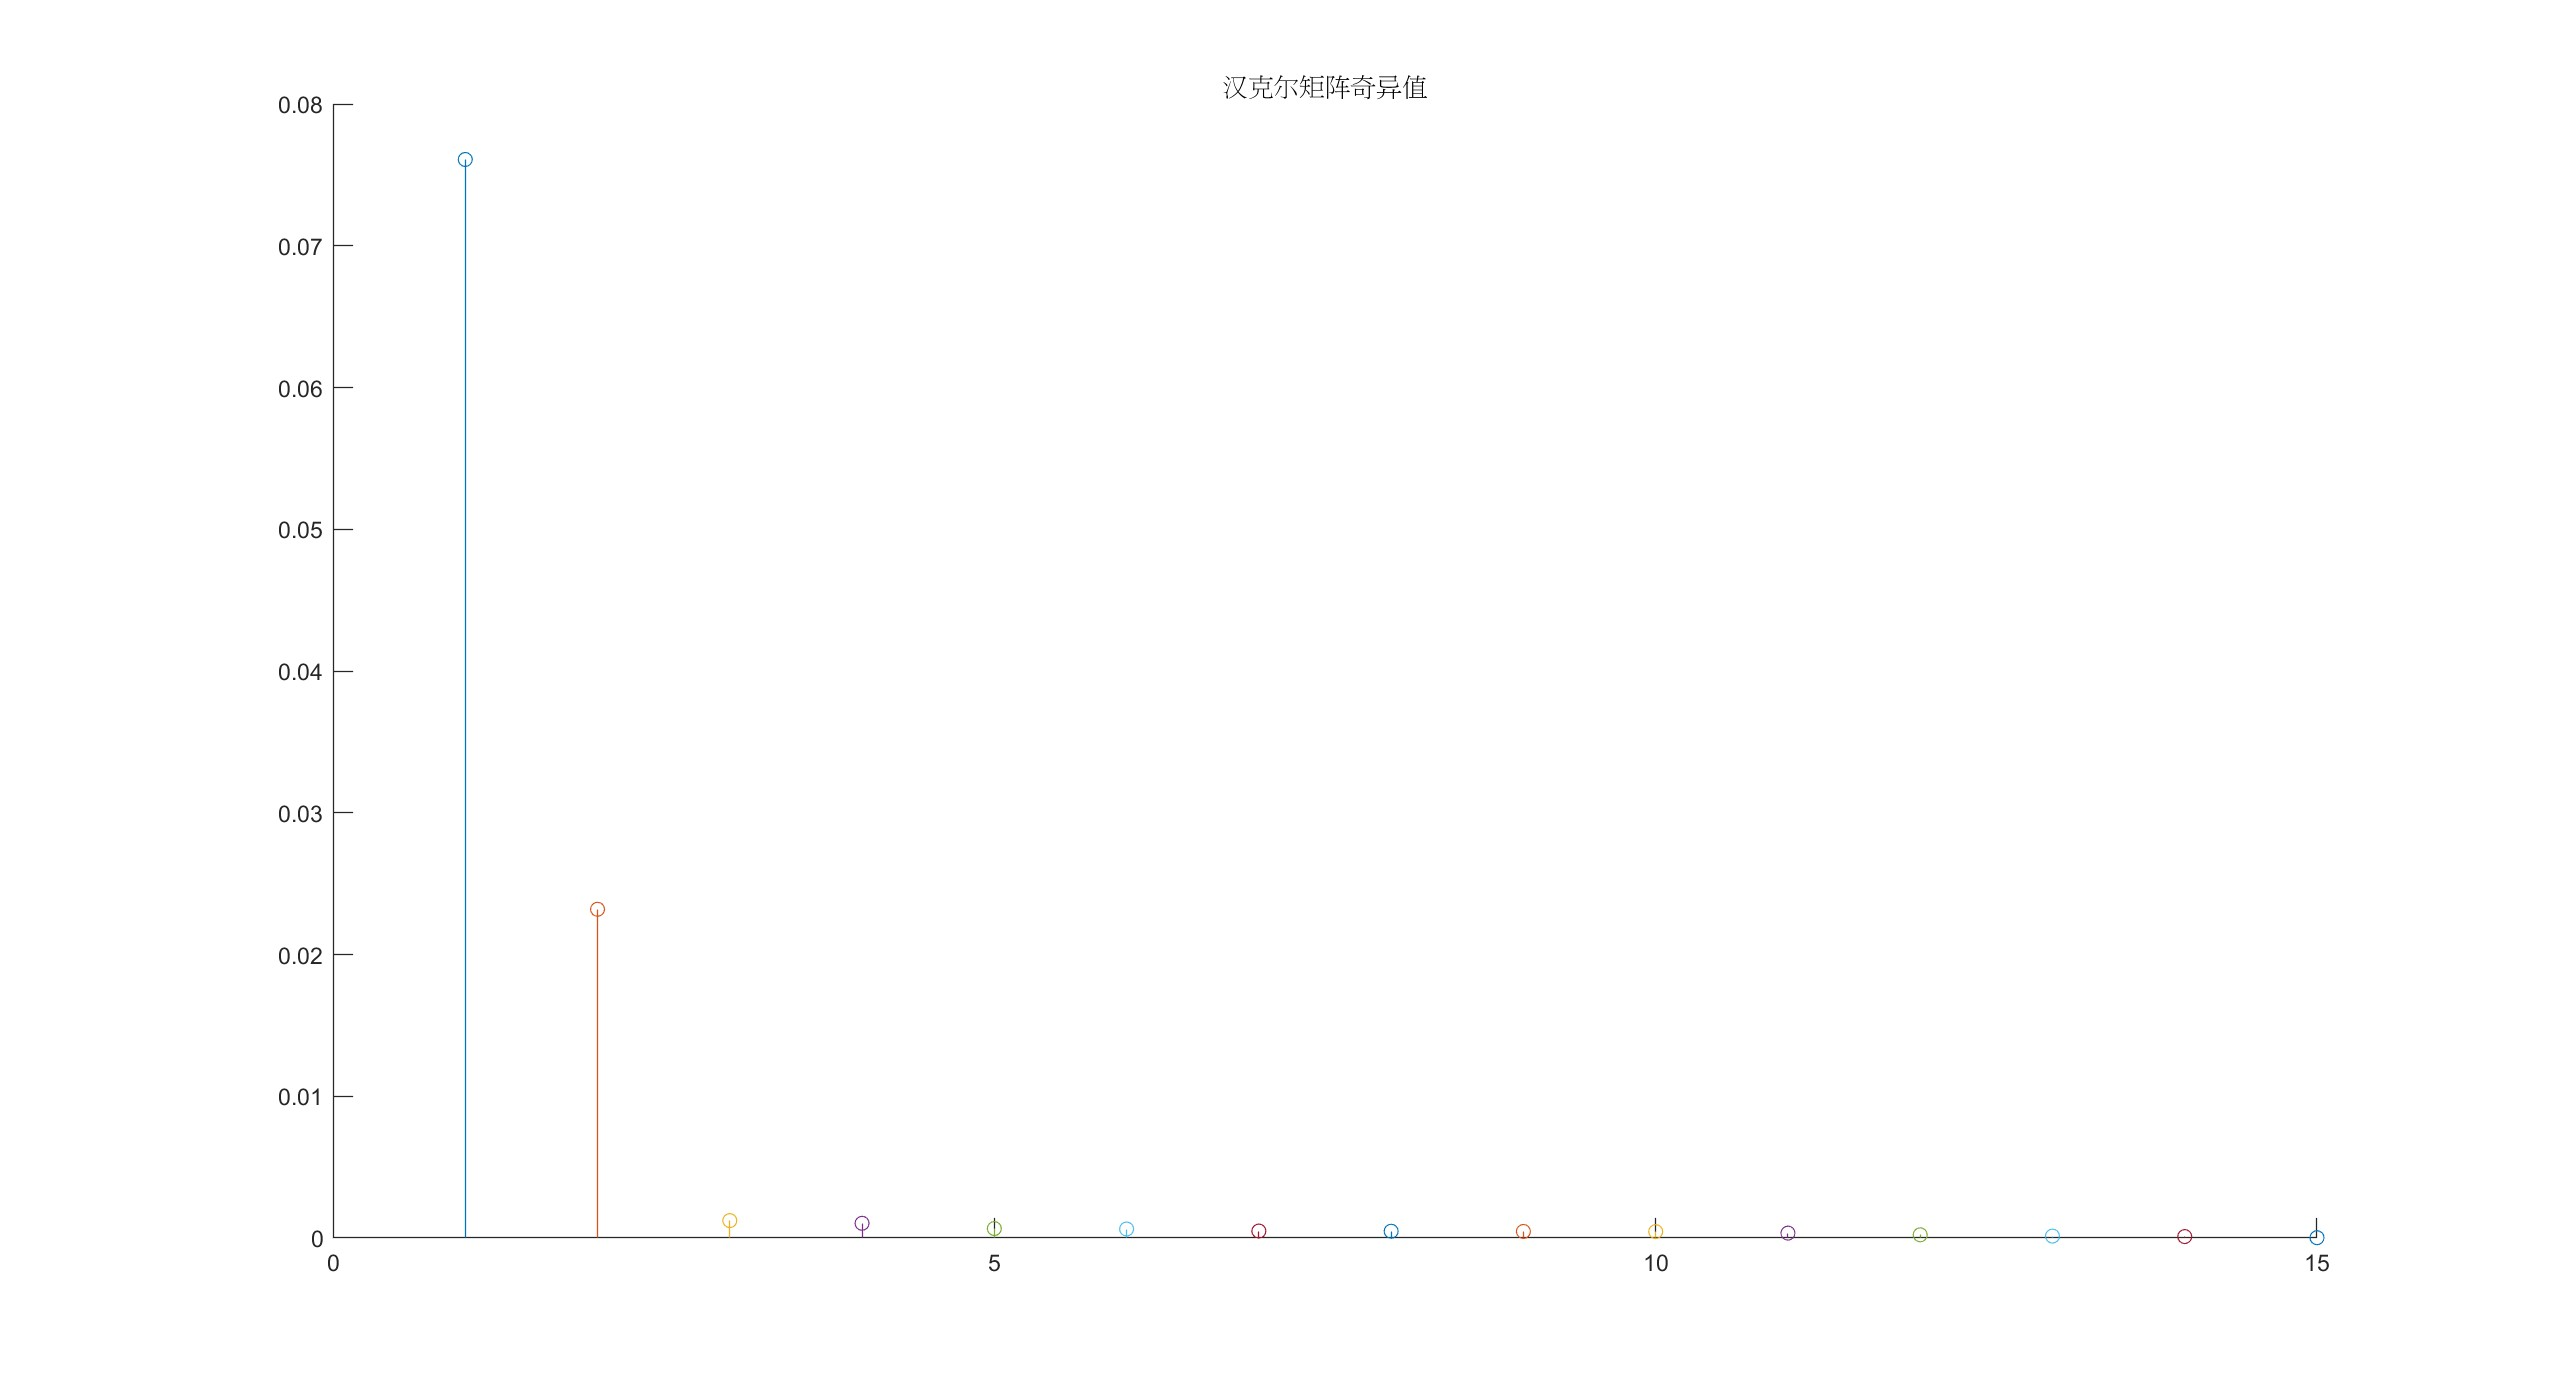
\includegraphics[width=\textwidth]
        {图片/D轴工作点4V奇异值分解图.jpg}
        \caption{D轴工作点4V奇异值分解图}
    \end{minipage}
    \begin{minipage}{0.5\textwidth}
        \centering
        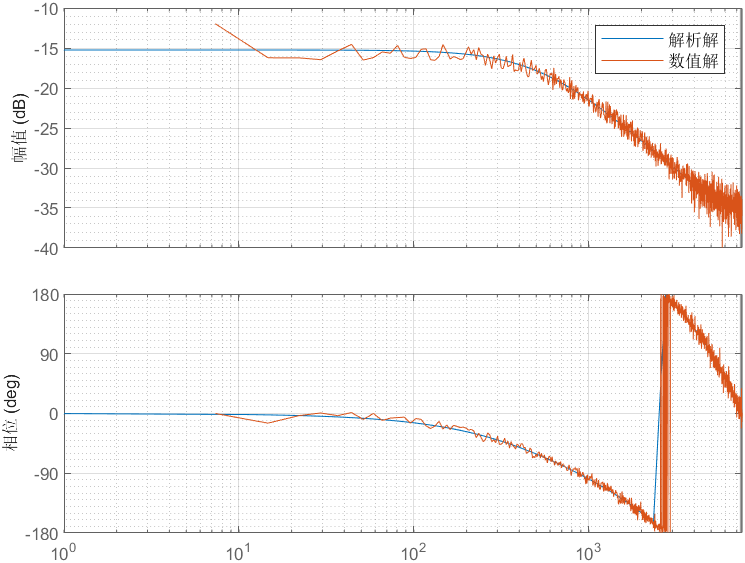
\includegraphics[width=\textwidth]
        {图片/D轴工作点4V数值解和解析解对比.jpg}
        \caption{D轴工作点4V数值解和解析解对比}
    \end{minipage}
\end{figure}

工作点-2V时，得到的Hankel矩阵奇异值分解和频域响应对比如下图所示。
数值解与解析解的幅频相关系数为98.88178\(\%\)，
相频相关系数为99.89867\(\%\)，拟合优度85.55227\(\%\)。解析解传递函数为
\(G(z)=\cfrac{0.00003966  + 0.00002372 z^{-1} + 0.0287z^{-2}}{1 - 0.7951 z^{-1} - 0.03771z^{-2}}\)，两个极点为
0.8400和-0.0499。得到-2V工作点下D轴同步电感为\(L_d=2.17947\textrm{mH}\)。
\begin{figure}[H]
    \begin{minipage}{0.5\textwidth}
        \centering
        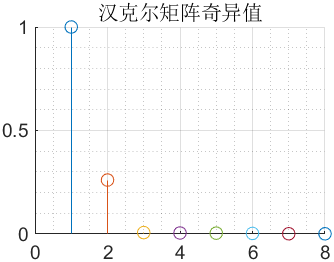
\includegraphics[width=\textwidth]
        {图片/D轴工作点-2V奇异值分解图.jpg}
        \caption{D轴工作点-2V奇异值分解图}
    \end{minipage}
    \begin{minipage}{0.5\textwidth}
        \centering
        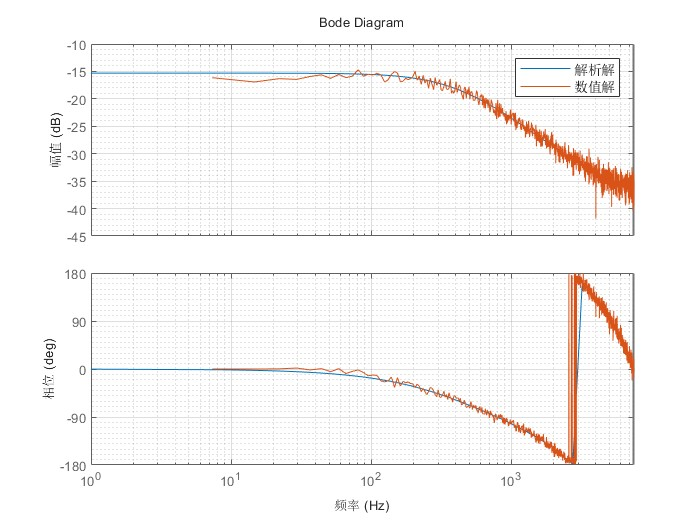
\includegraphics[width=\textwidth]
        {图片/D轴工作点-2V数值解和解析解对比.jpg}
        \caption{D轴工作点-2V数值解和解析解对比}
    \end{minipage}
\end{figure}

工作点-4V时，得到的Hankel矩阵奇异值分解和频域响应对比如下图所示。
数值解与解析解的幅频相关系数为98.73410\(\%\)，
相频相关系数为99.88621\(\%\)，拟合优度84.88066\(\%\)。解析解传递函数为
\(G(z)=\cfrac{0.00005562  - 0.0000877 z^{-1} + 0.02779z^{-2}}{1 - 0.7927 z^{-1} - 0.0462z^{-2}}\)，两个极点为
0.8472和-0.0545。得到-4V工作点下D轴同步电感为\(L_d=2.29122\textrm{mH}\)。
\begin{figure}[H]
    \begin{minipage}{0.5\textwidth}
        \centering
        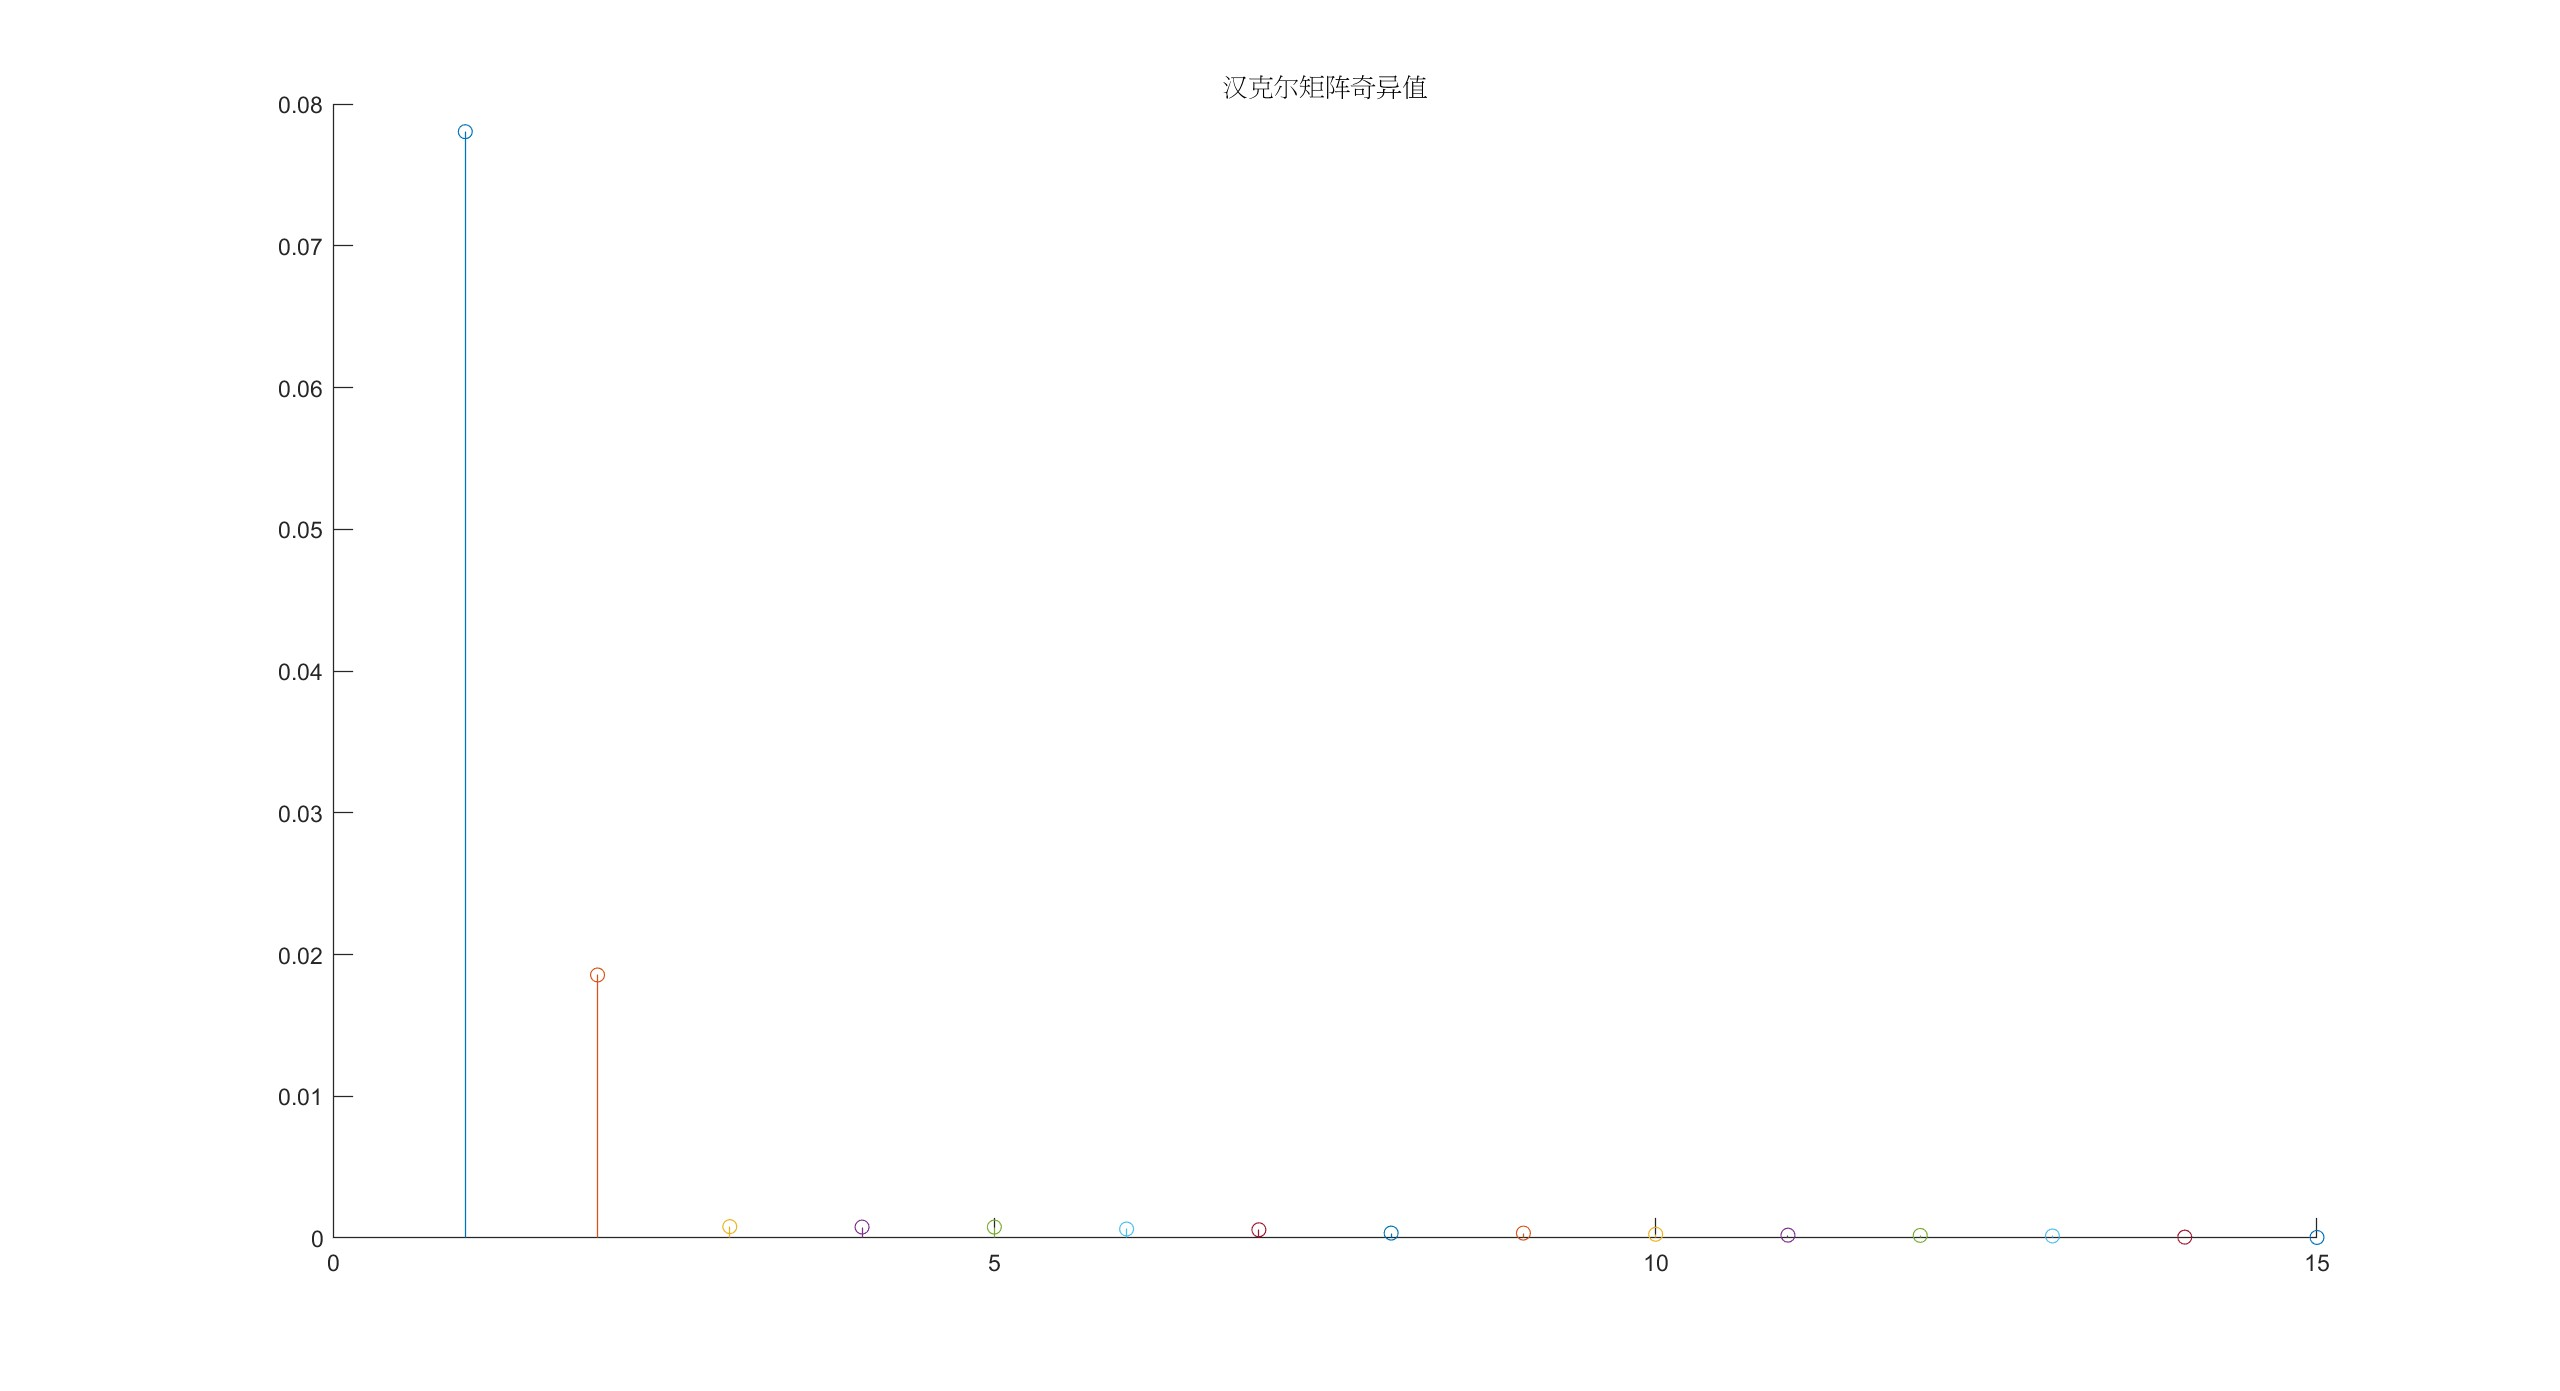
\includegraphics[width=\textwidth]
        {图片/D轴工作点-4V奇异值分解图.jpg}
        \caption{D轴工作点-4V奇异值分解图}
    \end{minipage}
    \begin{minipage}{0.5\textwidth}
        \centering
        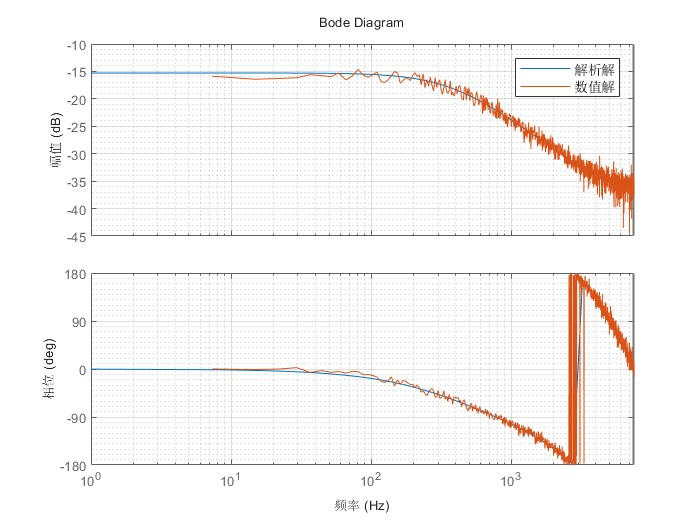
\includegraphics[width=\textwidth]
        {图片/D轴工作点-4V数值解和解析解对比.jpg}
        \caption{D轴工作点-4V数值解和解析解对比}
    \end{minipage}
\end{figure}

将上述五个工作点的D轴辨识结果汇总如下表所示。
\begin{table}[H]
    \centering
    \begin{tabular}{|c|c|c|c|c|}
        \hline
        工作点 & 幅频相关系数 & 相频相关系数 & 拟合优度 & \(L_d\)辨识值（mH）\\
        \hline
        \(U_d=-4\text{V}\)  & 98.73410\% & 99.88621\% & 84.88066\% & 2.29122\\
        \hline
        \(U_d=-2\text{V}\)  & 98.88178\% & 99.89867\% & 85.55227\% & 2.17947\\
        \hline
        \(U_d=0\text{V}\)   & 98.89805\% & 99.90722\% & 86.40194\% & 1.86152\\
        \hline
        \(U_d=2\text{V}\)   & 98.94669\% & 99.94114\% & 87.09381\% & 1.80467\\
        \hline
        \(U_d=4\text{V}\)   & 98.97066\% & 99.91828\% & 86.93735\% & 1.63713\\
        \hline
    \end{tabular}
    \caption{D轴各工作点HK辨识结果汇总}
    \label{tab:D轴各工作点辨识结果汇总}
\end{table}

根据HK伪随机辨识结果可以发现，随着工作点电压，也就是伪随机信号直流分量的增加，D轴同步电感辨识结果随之减小，
这与永磁同步电机的数学模型是匹配的，并非是算法问题，
接下来对此进行分析。

\subsubsection{工作点变化对D轴电感辨识结果的影响}

铁磁材料的磁化曲线如下图所示。可以发现，随着外界激发磁场强度H增大，磁感应强度B呈现出快速升高后逐渐饱和的现象，磁导率\(\mu=\cfrac{B}{H}\)
则呈现出先快速升高到极点后迅速下降的特点。磁导率的最大值称为铁磁材料的膝点，越过膝点就称为进入了磁饱和区，并且越过膝点越远，磁饱和程度越高。
\begin{figure}[H]
    \centering
    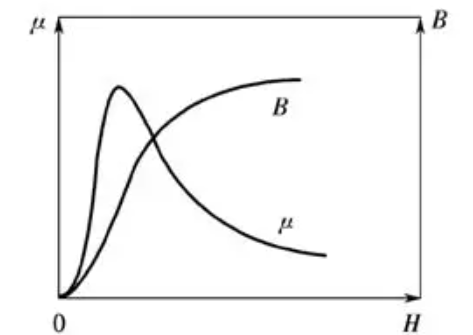
\includegraphics[width=0.4\textwidth]
    {图片/铁磁材料的磁化曲线.png}
    \caption{铁磁材料的磁化曲线}
\end{figure}

对于大部分永磁同步电机，转子磁场主要由永磁体提供，本身磁场强度较高，已进入磁饱和区。在D轴上，设永磁体磁动势为\(F_{c}\)为定值，
D轴电流产生的磁动势为\(F_{d}=Ni_d\)，其中\(N\)表示等效匝数。根据磁路欧姆定律，磁通量可以表示为：
\begin{equation*}
    \varPhi=\cfrac{F_{c}+F_{d}}{R_m}=\cfrac{F_{c}+Ni_d}{R_m}=\cfrac{\mu S(F_c+Ni_{d})}{l_c}
\end{equation*}

其中\(R_m\)为磁阻，表达式为\(R_m=\cfrac{l}{\mu S}\)，其中\(\mu\)表示磁导率，\(l\)表示磁路长度，\(S\)表示磁路横截面积。
磁阻主要分为三个部分：永磁体磁阻\(R_{pm}\)，气隙磁阻\(R_g\)，定子铁心磁阻\(R_{Fe}=\cfrac{l_{Fe}}{\mu_{Fe} S_{Fe}}\)。
其中永磁体磁阻和气隙磁阻可视为常数，和为\(R_c\)，定子铁心磁阻由于不同工作点的\(i_d\)不同而会发生变化。
因此将磁阻改写为\(R_m=R_{c}+\cfrac{l_{Fe}}{\mu S_{Fe}}\)。

HK辨识方法是在工作点附近的局部线性化结果，此时辨识得到的电感为增量电感，即\(L_d=\cfrac{\partial\psi}{\partial i_d}\)，其中
磁链为\(\psi=N\varPhi\)。由于等效匝数\(N\)不变，因此辨识电感为\(L_d=N\cfrac{d\varPhi}{di_d}\)。

代入磁路欧姆定律方程可得\(L_d=N\cfrac{d}{di_d}(\cfrac{F_e+Ni_d}{R_c+R_{Fe}})\)，分别求取微分可得
\(L_d=-N\cfrac{F_e}{R_c+R_{Fe}}\cfrac{dR_{Fe}}{di_d}+N^2\cfrac{(R_c+R_{Fe})-i_d\frac{dR_{Fe}}{di_d}}{(R_c+R_{Fe})^2}\)，整理得到：
\begin{equation*}
    L_d=\cfrac{N^2}{R_c+R_{Fe}}-\cfrac{N(F_e+Ni_d)}{(R_c+R_{Fe})^2}\cfrac{dR_{Fe}}{di_d}
\end{equation*}

当工作点电压升高，\(u_d>0\)时，电流工作点\(i_d>0\)，表现为助磁，加深磁场的饱和程度，使得磁导率\(\mu\)进一步下降，
定子铁心磁阻\(R_{Fe}=\cfrac{l_{Fe}}{\mu_{Fe} S_{Fe}}\)快速升高。这会带来两个结果：
第一，由于\(R_{Fe}\)迅速升高，使得\(\cfrac{N^2}{R_c+R_{Fe}}\)快速降低；第二，由于\(R_{Fe}\)呈现为上升趋势，因此
\(\cfrac{dR_{Fe}}{di_d}>0\)并且\(i_d\)升高，使得\(\cfrac{N(F_e+Ni_d)}{(R_c+R_{Fe})^2}\cfrac{dR_{Fe}}{di_d}\)项升高。
最终使得辨识得到的\(L_d\)呈现处随工作点电压升高而降低的现象。

而当工作电压降低，\(u_d<0\)时，电流工作点\(i_d<0\)，表现为去磁，减少磁场的饱和程度。在膝点之前磁导率\(\mu\)会随着\(u_d\)进一步的下降
而升高，也就能看到\(L_d\)随工作点电压降低而升高的现象。若\(i_d\)反向足够大，则会越过膝点，使得磁导率开始下降，\(L_d\)辨识结果降低。
但对于大部分永磁同步电机，若去磁电流过大，会使得永磁体产生不可逆的去磁，不利于电机工作，因此若进行磁场的弱磁或助磁控制，
需要谨慎选取给定电流，避免造成不可逆的永磁体损伤。

再次在多个工作点进行辨识，可以绘制得到D轴同步电感随工作点电压变化的关系图如下所示。考虑到噪声干扰和辨识偏差，据图可以认为，
上述定性推导是正确的，D轴同步电感辨识结果随工作点电压升高而降低为物理系统规律，并非算法误差。
\begin{figure}[H]
    \centering
    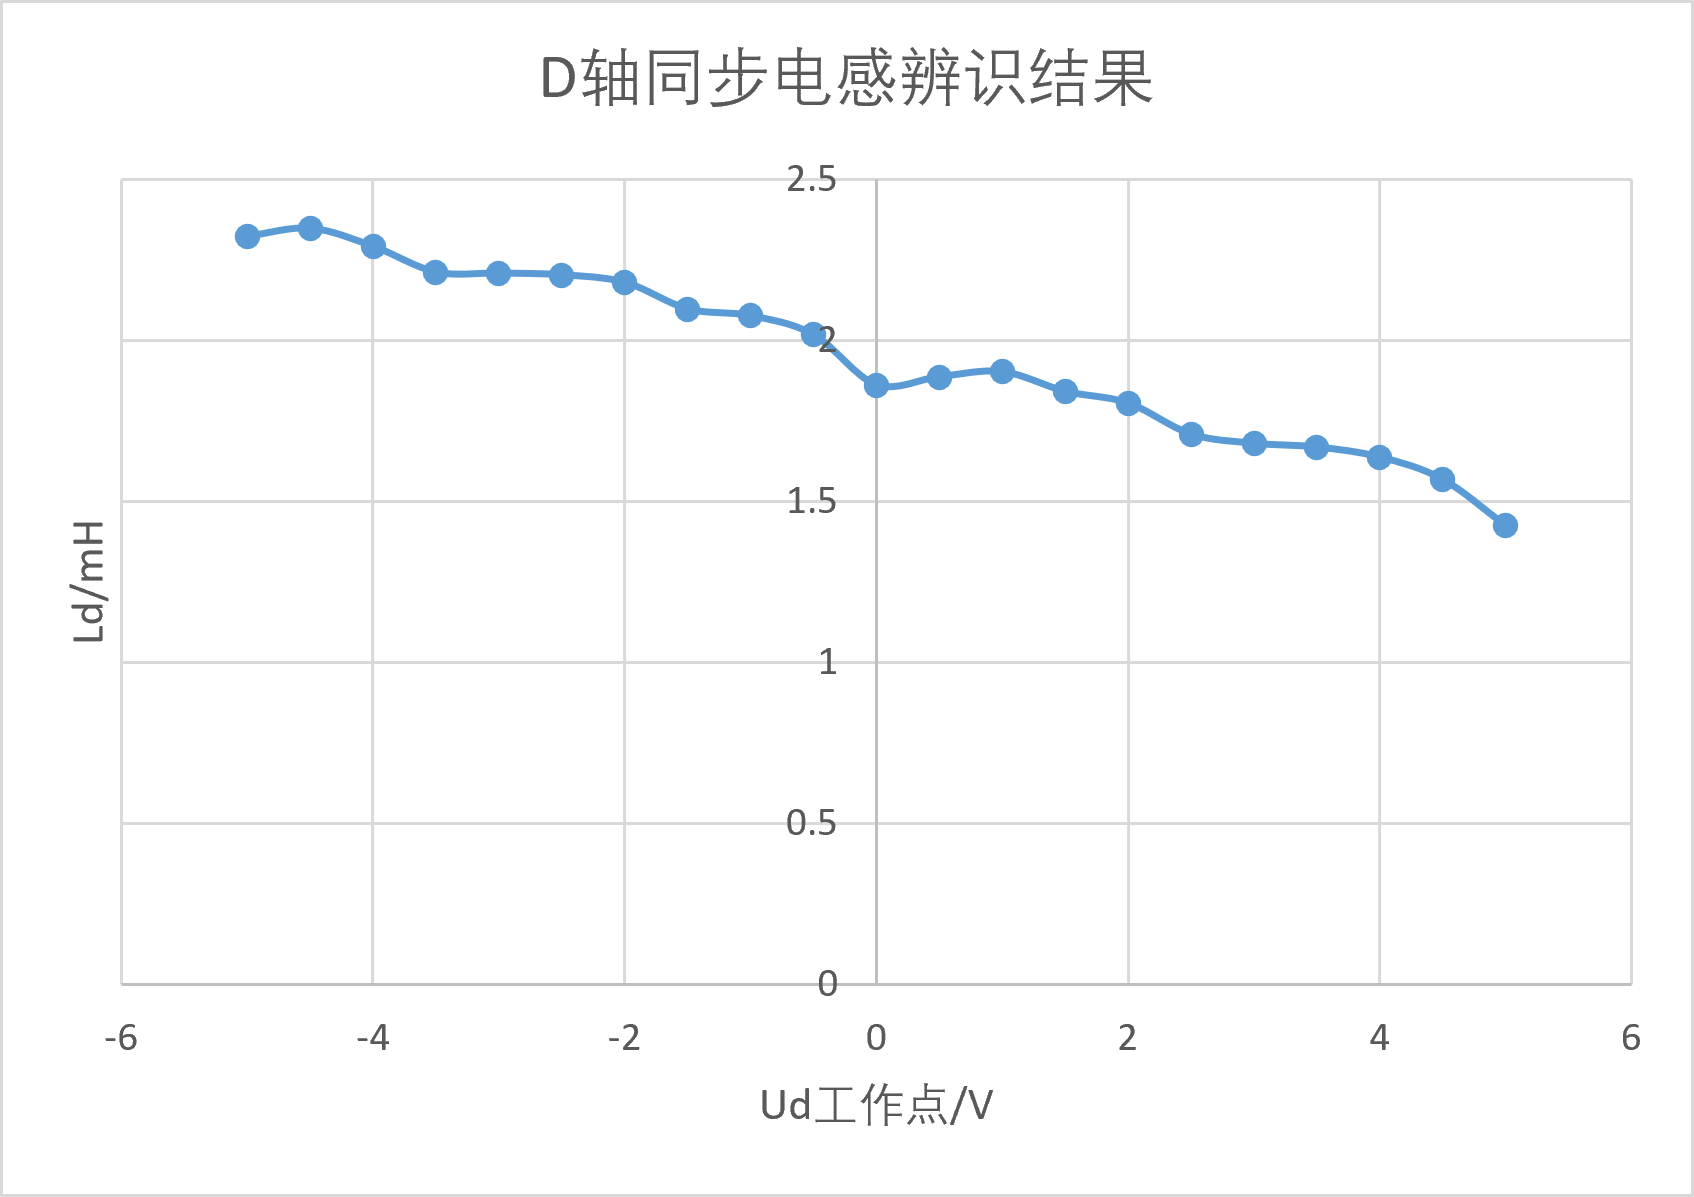
\includegraphics[width=0.8\textwidth]
    {图片/D轴同步电感辨识曲线.png}
    \caption{D轴同步电感辨识曲线}
\end{figure}

考虑到在大部分FOC控制中选取\(i_d=0\)作为工作点，因此取\(u_d=0\)时的辨识结果为如下，
满足相间电感估计得到的同步电感范围\(L_d\in(1.76917,1.94354)\textrm{mH}\)。
\begin{equation*}
    L_{dO}=1.86152\textrm{mH}
\end{equation*}

\subsection{永磁体磁链测量\label{sec:永磁体磁链测量}}

基于相电阻\(R_s\)和D轴同步电感\(L_d\)的辨识结果，可以在稳态情况下实现对永磁体磁链\(\psi_m\)的辨识。

对于电路方程\eqref{eq:同步坐标系下电路方程}，只考虑Q轴情况下可以改写为：
\begin{equation*}
    u_q=R_si_q+L_q\cfrac{di_q}{dt}+\omega_e(L_di_d+\psi_m)
\end{equation*}

进行\(u_q\)给定的开环拖动，在稳态情况下\(i_q\)不再变化，因此\(\cfrac{di_q}{dt}=0\)，可以将Q轴电路方程改写为
\(u_q=R_si_q+\omega_e(L_di_d+\psi_m)\)，可以变形为：
\begin{equation*}
    \psi_m=\cfrac{u_q-R_si_q}{\omega_e}-L_di_d
\end{equation*}

其中\(u_q\)为给定量，\(R_s,L_d\)通过上述两节完成了辨识，可以视为定值，\(i_d,i_q,\omega_e\)均可以进行测量。
按照上式实时计算永磁体磁链并回传到上位机，期间调整\(u_q\)以验证各个工作点下工作的一致性，波形如下图所示。
\begin{figure}[H]
    \centering
    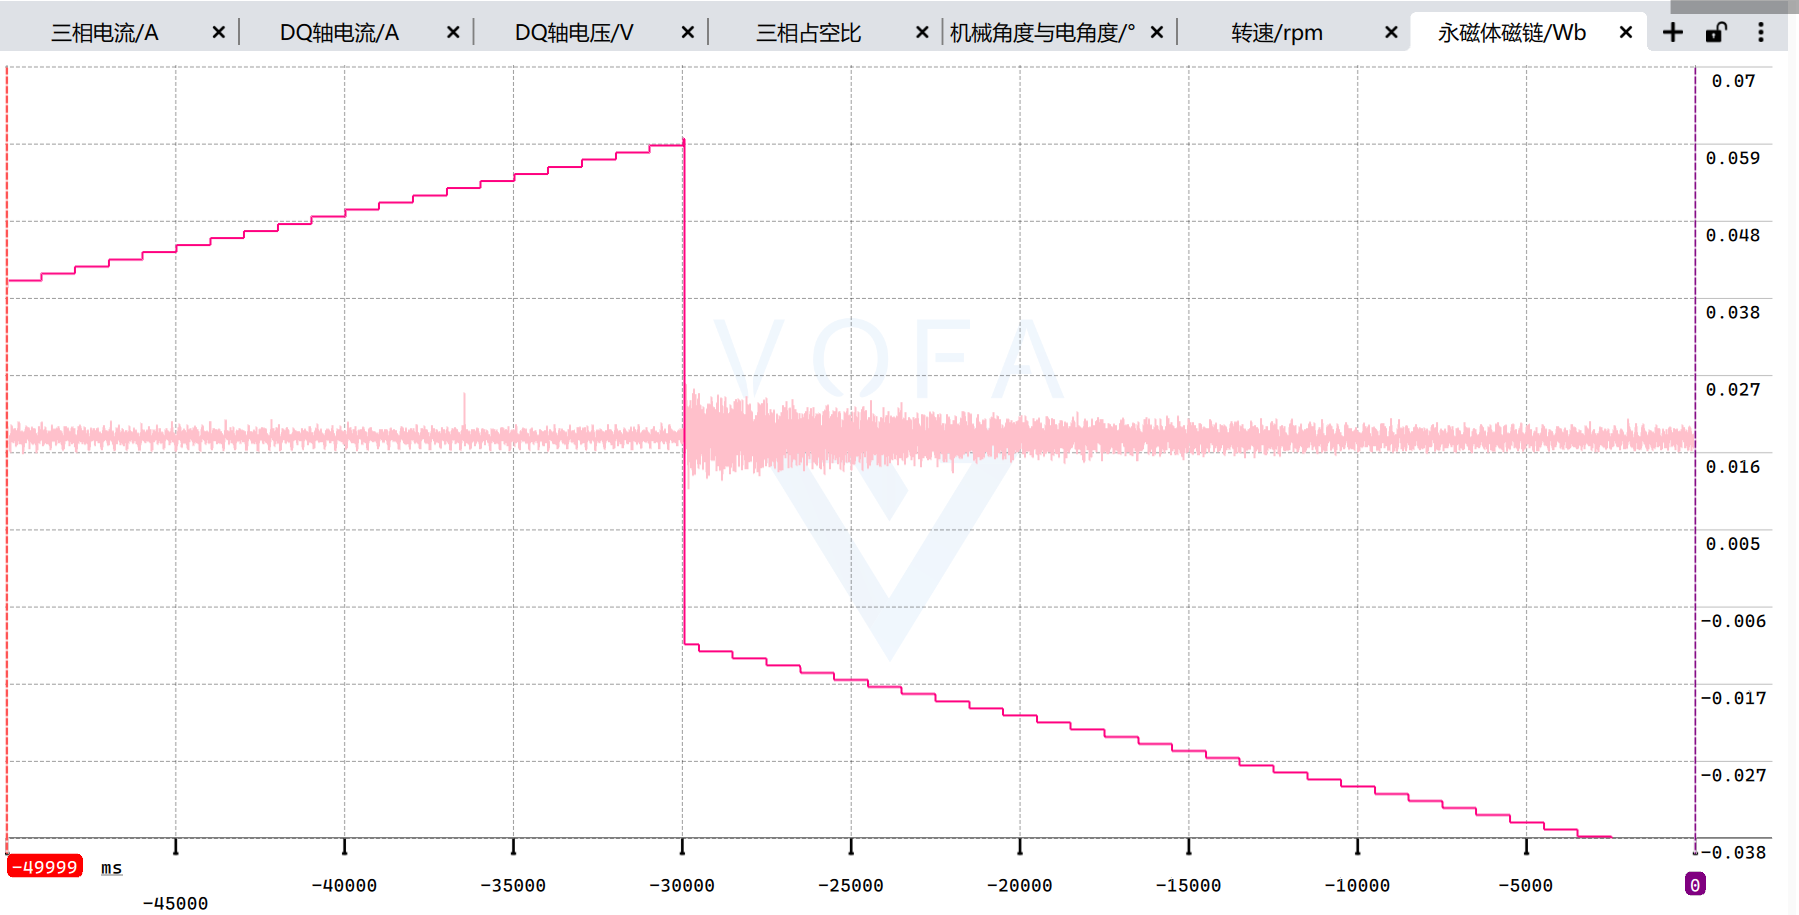
\includegraphics[width=0.8\textwidth]
    {图片/永磁体磁链辨识波形.png}
    \caption{永磁体磁链辨识波形（绿：\(u_q\)，红：\(\psi_m\)）}
\end{figure}

可以发现，当\(u_q\)给定较小时，辨识得到的\(\psi_m\)变化剧烈，这主要是因为\(u_q\)较小时转速较慢，
\(\omega_e\)较小，使得测量误差和噪声被由于分母太小而被放大。随着\(u_q\)给定值提高，电机转速升高，信噪比会逐步提高，
对永磁体磁链的辨识结果逐渐收敛到特定值。
取\(2<|u_q|<5.5\)，以0.1V为单位绘制\(\psi_m\)随\(u_q\)变化的关系图如下所示。
\begin{figure}[H]
    \centering
    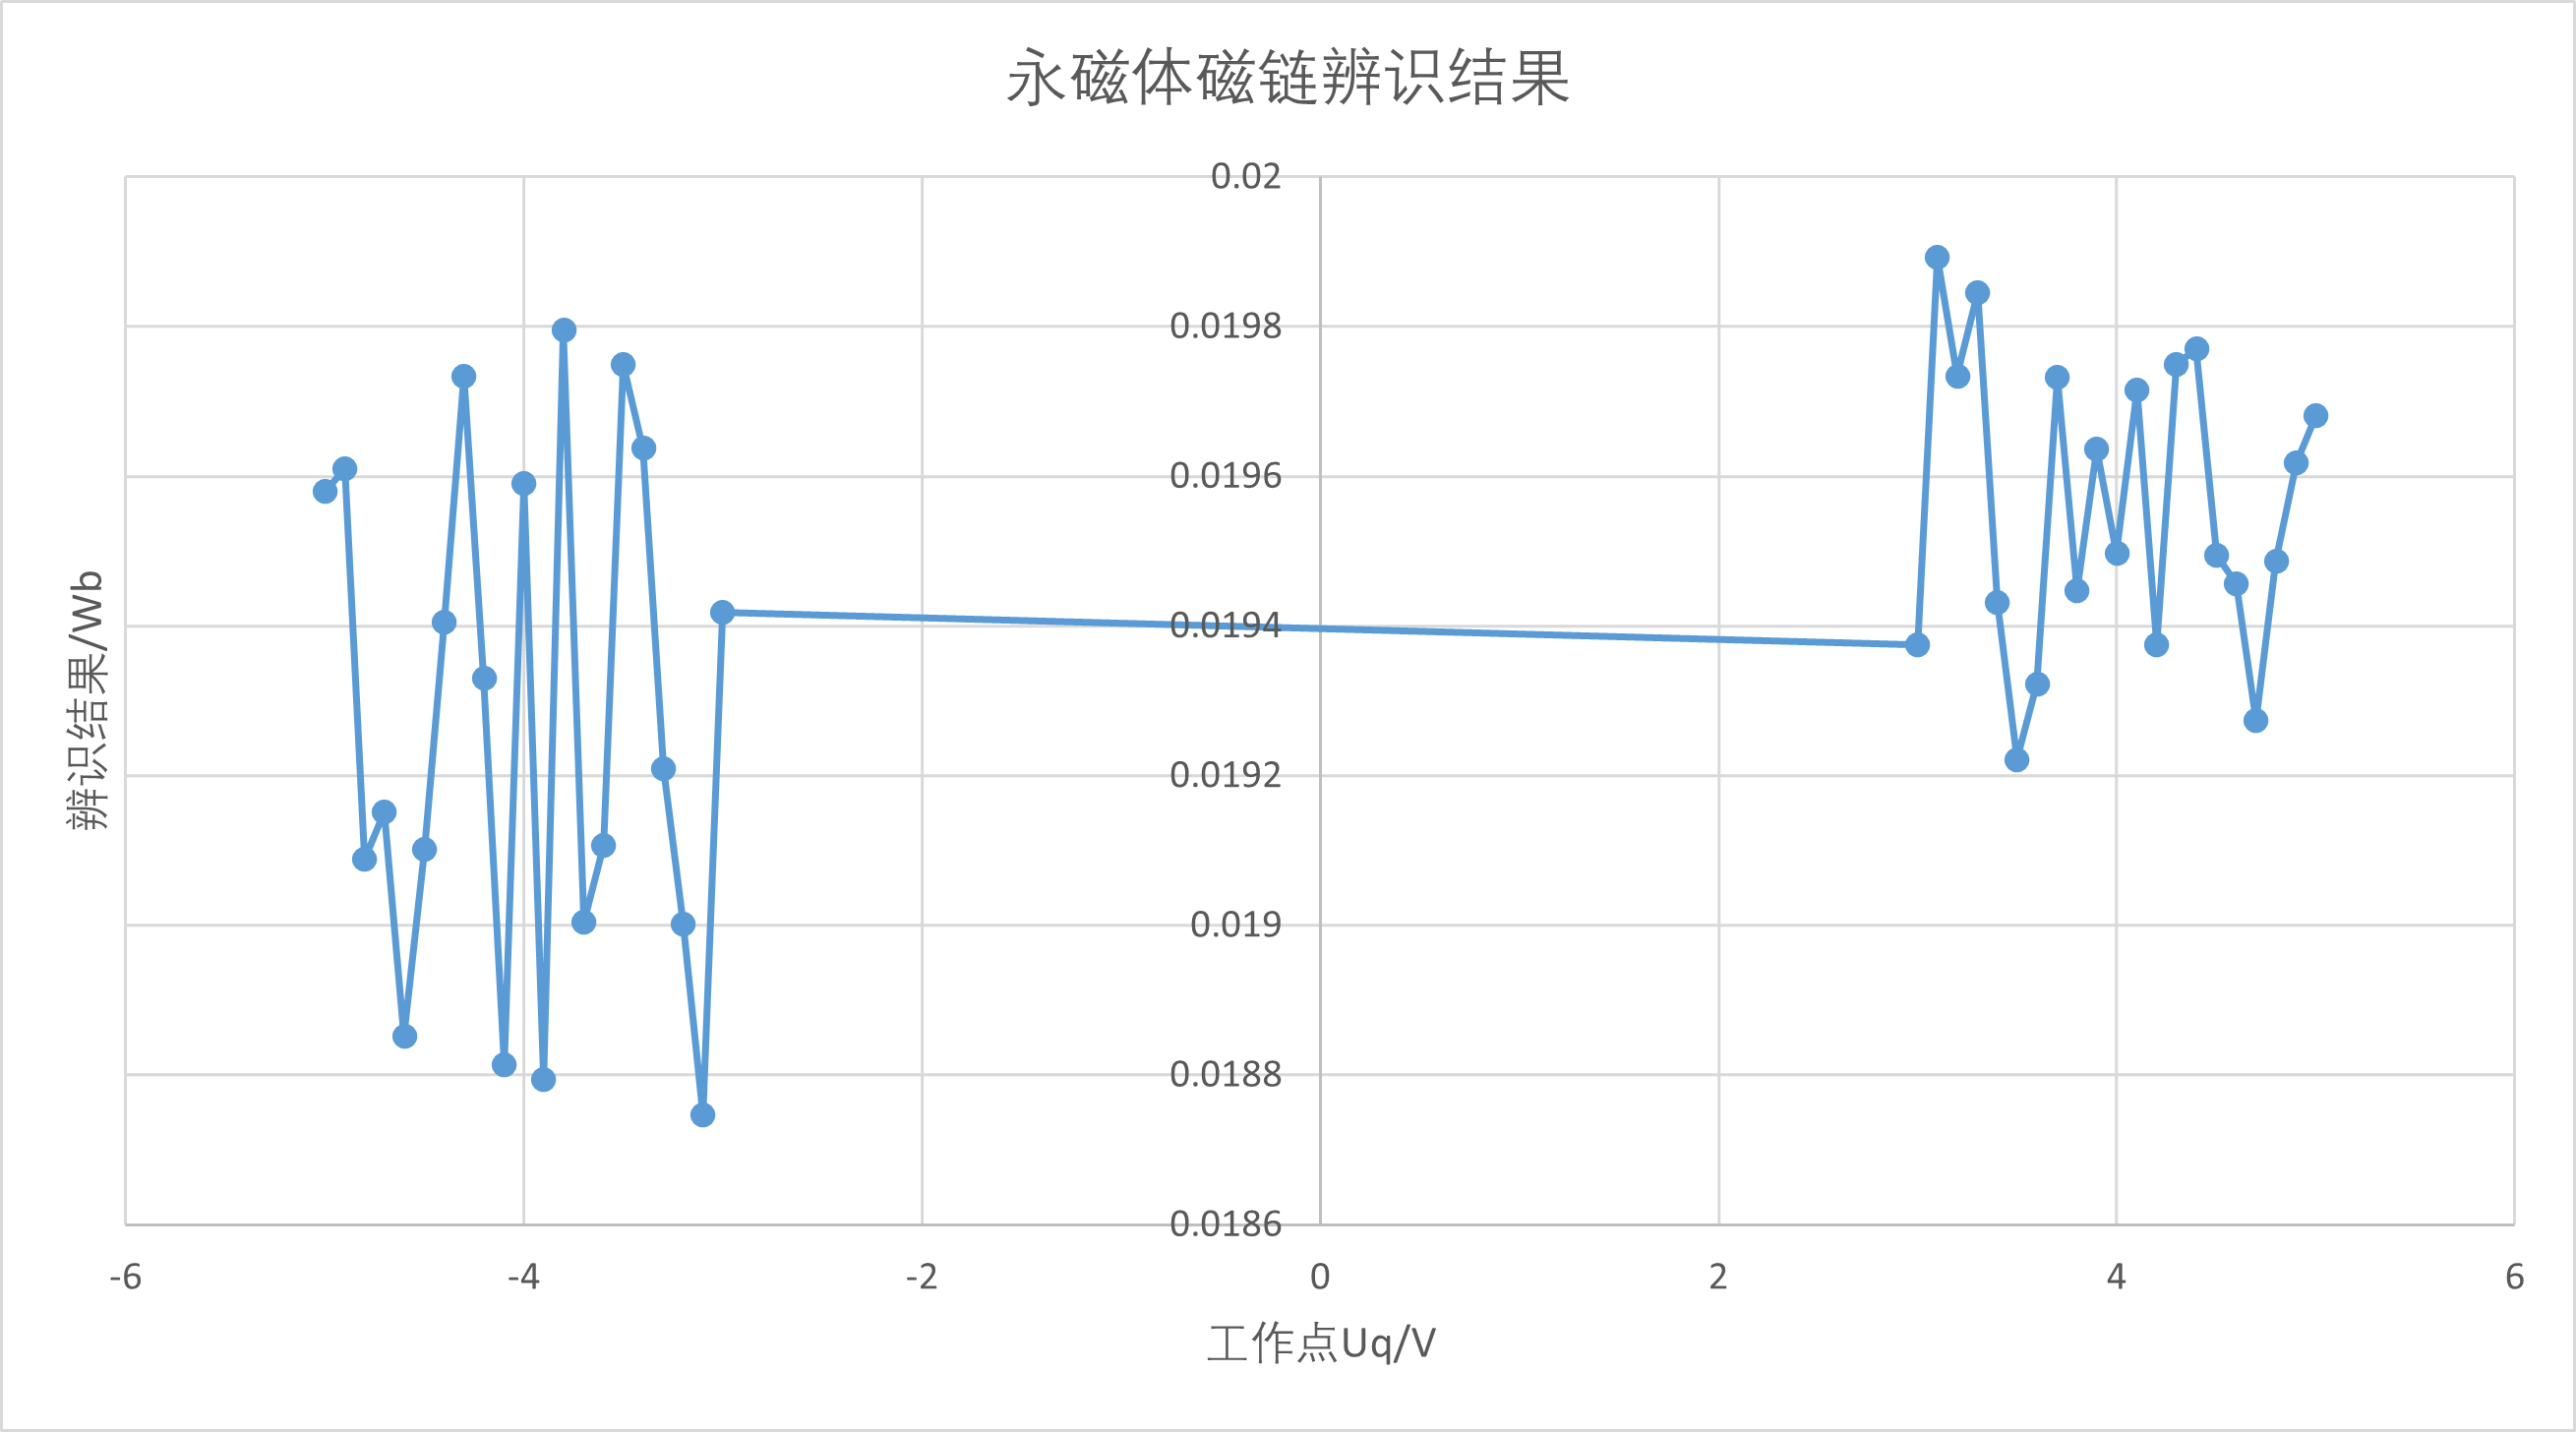
\includegraphics[width=0.8\textwidth]
    {图片/永磁体磁链辨识结果.png}
    \caption{永磁体磁链辨识结果}
\end{figure}

计算得到平均值为9.65548mWb，标准差0.000172651，相对标准误差为1.79\(\%\)，数据的精准度较高，可以近似认为在各个工作点附近永磁体磁链
不变，符合物理规律。

因此永磁体磁链辨识结果为：
\begin{equation*}
    \psi_{mO}=9.65548\textrm{mWb}
\end{equation*}

\subsection{Q轴同步电感辨识}
最后进行Q轴同步电感的辨识。根据电路方程有：
\begin{equation*}
    u_q=R_si_q+L_q\cfrac{di_q}{dt}+\omega_e(L_di_d+\psi_m)
\end{equation*}

理想情况下，若能保持严格锁定转轴，则\(\omega_e=0\)，Q轴可以退化为与进行D轴电感辨识时类似的一阶RL电路。但由于电磁转矩
\(T_e=\cfrac32pi_qi_d(L_d-L_q)+\cfrac32\psi_mpi_q\propto i_q\)
，一旦\(i_q\)产生响应就会差生电磁转矩。并且在高频变化的伪随机\(u_q\)
作用下，会产生高频变化的\(i_q\)，电磁转矩也随之发生变化，这对锁轴的提出了很高要求。

此外，由于电机磁路不对称有\(L_q\ge L_d\)，这点从式\eqref{eq:同步电感定义式}可以看出，
主要是因为D轴定义为与永磁体磁链平行的方向，磁饱和程度较高。
而时间常数\(\tau=\cfrac LR\)，因此Q轴时间常数一般会比D轴更大，脉冲响应需要更长时间
达到稳态，因此可以适当增大Hankel矩阵阶次到15。而系统阶次，考虑到理想情况下PWM模态的贡献，选取为2。
此外由于DQ轴的磁路不对称，Q轴由于反电动势存在和较大的同步电感存在，使得Q轴的电流响应幅度小于D轴，
为了获取较高的信噪比，需要增大激励电压的幅值，因此选取伪随机参数为幅值2，工作点0。

\subsubsection{电气锁轴方法\label{sec:电气锁轴方法}}
首先尝试进行电气锁轴，其主要原理是通过\(i_d\)的电流闭环，产生一个方向恒定的磁场吸引转子与之对齐，并且通过将\(i_d\)闭环到
较高水平确保能够较为牢固的吸住转子，在此基础上进行Q轴的伪随机辨识。下图是D轴电流闭环\(i_d=0.5A\)的HK辨识结果。
\begin{figure}[H]
    \centering
    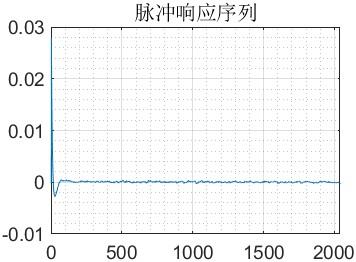
\includegraphics[width=0.8\textwidth]
    {图片/电气锁轴脉冲响应序列.jpg}
    \caption{电气锁轴脉冲响应序列}
\end{figure}

根据脉冲响应序列可以发现脉冲响应存在震荡，说明原系统存在欠阻尼的一对共轭极点。
进行奇异值分解和传递函数辨识结果如下所示。
\begin{figure}[H]
    \begin{minipage}{0.5\textwidth}
        \centering
        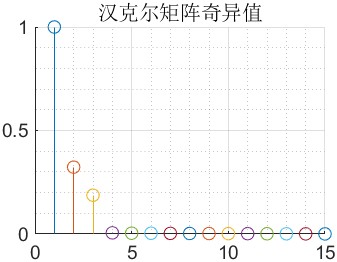
\includegraphics[width=\textwidth]
        {图片/电气锁轴奇异值分解图.jpg}
        \caption{电气锁轴奇异值分解图}
    \end{minipage}
    \begin{minipage}{0.5\textwidth}
        \centering
        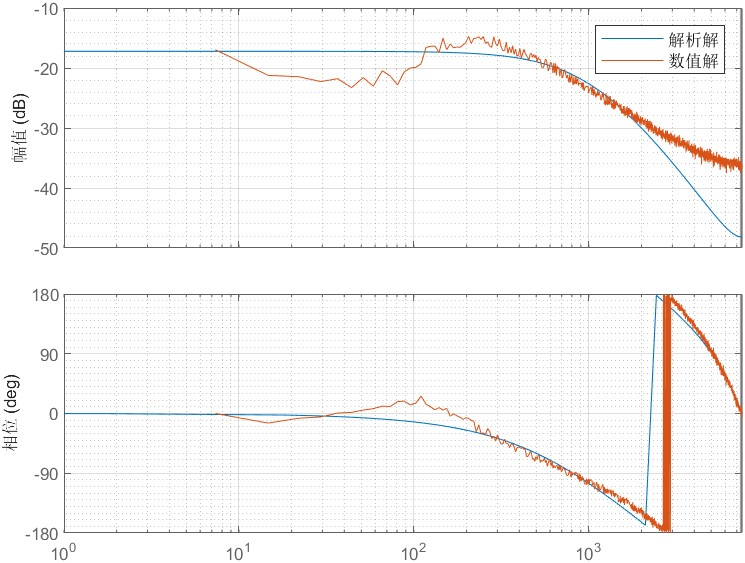
\includegraphics[width=\textwidth]
        {图片/电气锁轴数值解与解析解对比.jpg}
        \caption{电气锁轴数值解与解析解对比}
    \end{minipage}
\end{figure}

可以发现，电气锁轴不采用机械锁轴，难以确保转子锁定。而转子一旦开始转动，则PWM自身模态、Q轴RL电路模态、转动耦合模态
（主要由\(\omega_e(L_di_d+\psi_m)\)引起）等相互作用，
污染了辨识结果，使得难以从传递函数中提取出所需的信息。

\subsubsection{机械堵转方法\label{sec:机械堵转方法}}
接下来尝试机械堵转，辨识结果如下。
\begin{figure}[H]
    \centering
    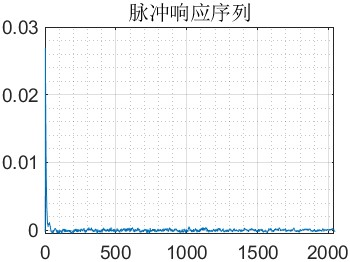
\includegraphics[width=0.8\textwidth]
    {图片/机械堵转脉冲响应序列.jpg}
    \caption{机械堵转脉冲响应序列}
\end{figure}

可以发现，通过机械堵转可以大幅降低脉冲响应中的震荡，使得辨识转动耦合模态含量降低。但由于无法严格锁轴，存在微动，因此无法完全杜绝
转动耦合模态带来的震荡。

对机械堵转进行奇异值分解和传递函数辨识，结果如下图所示
\begin{figure}[H]
    \begin{minipage}{0.5\textwidth}
        \centering
        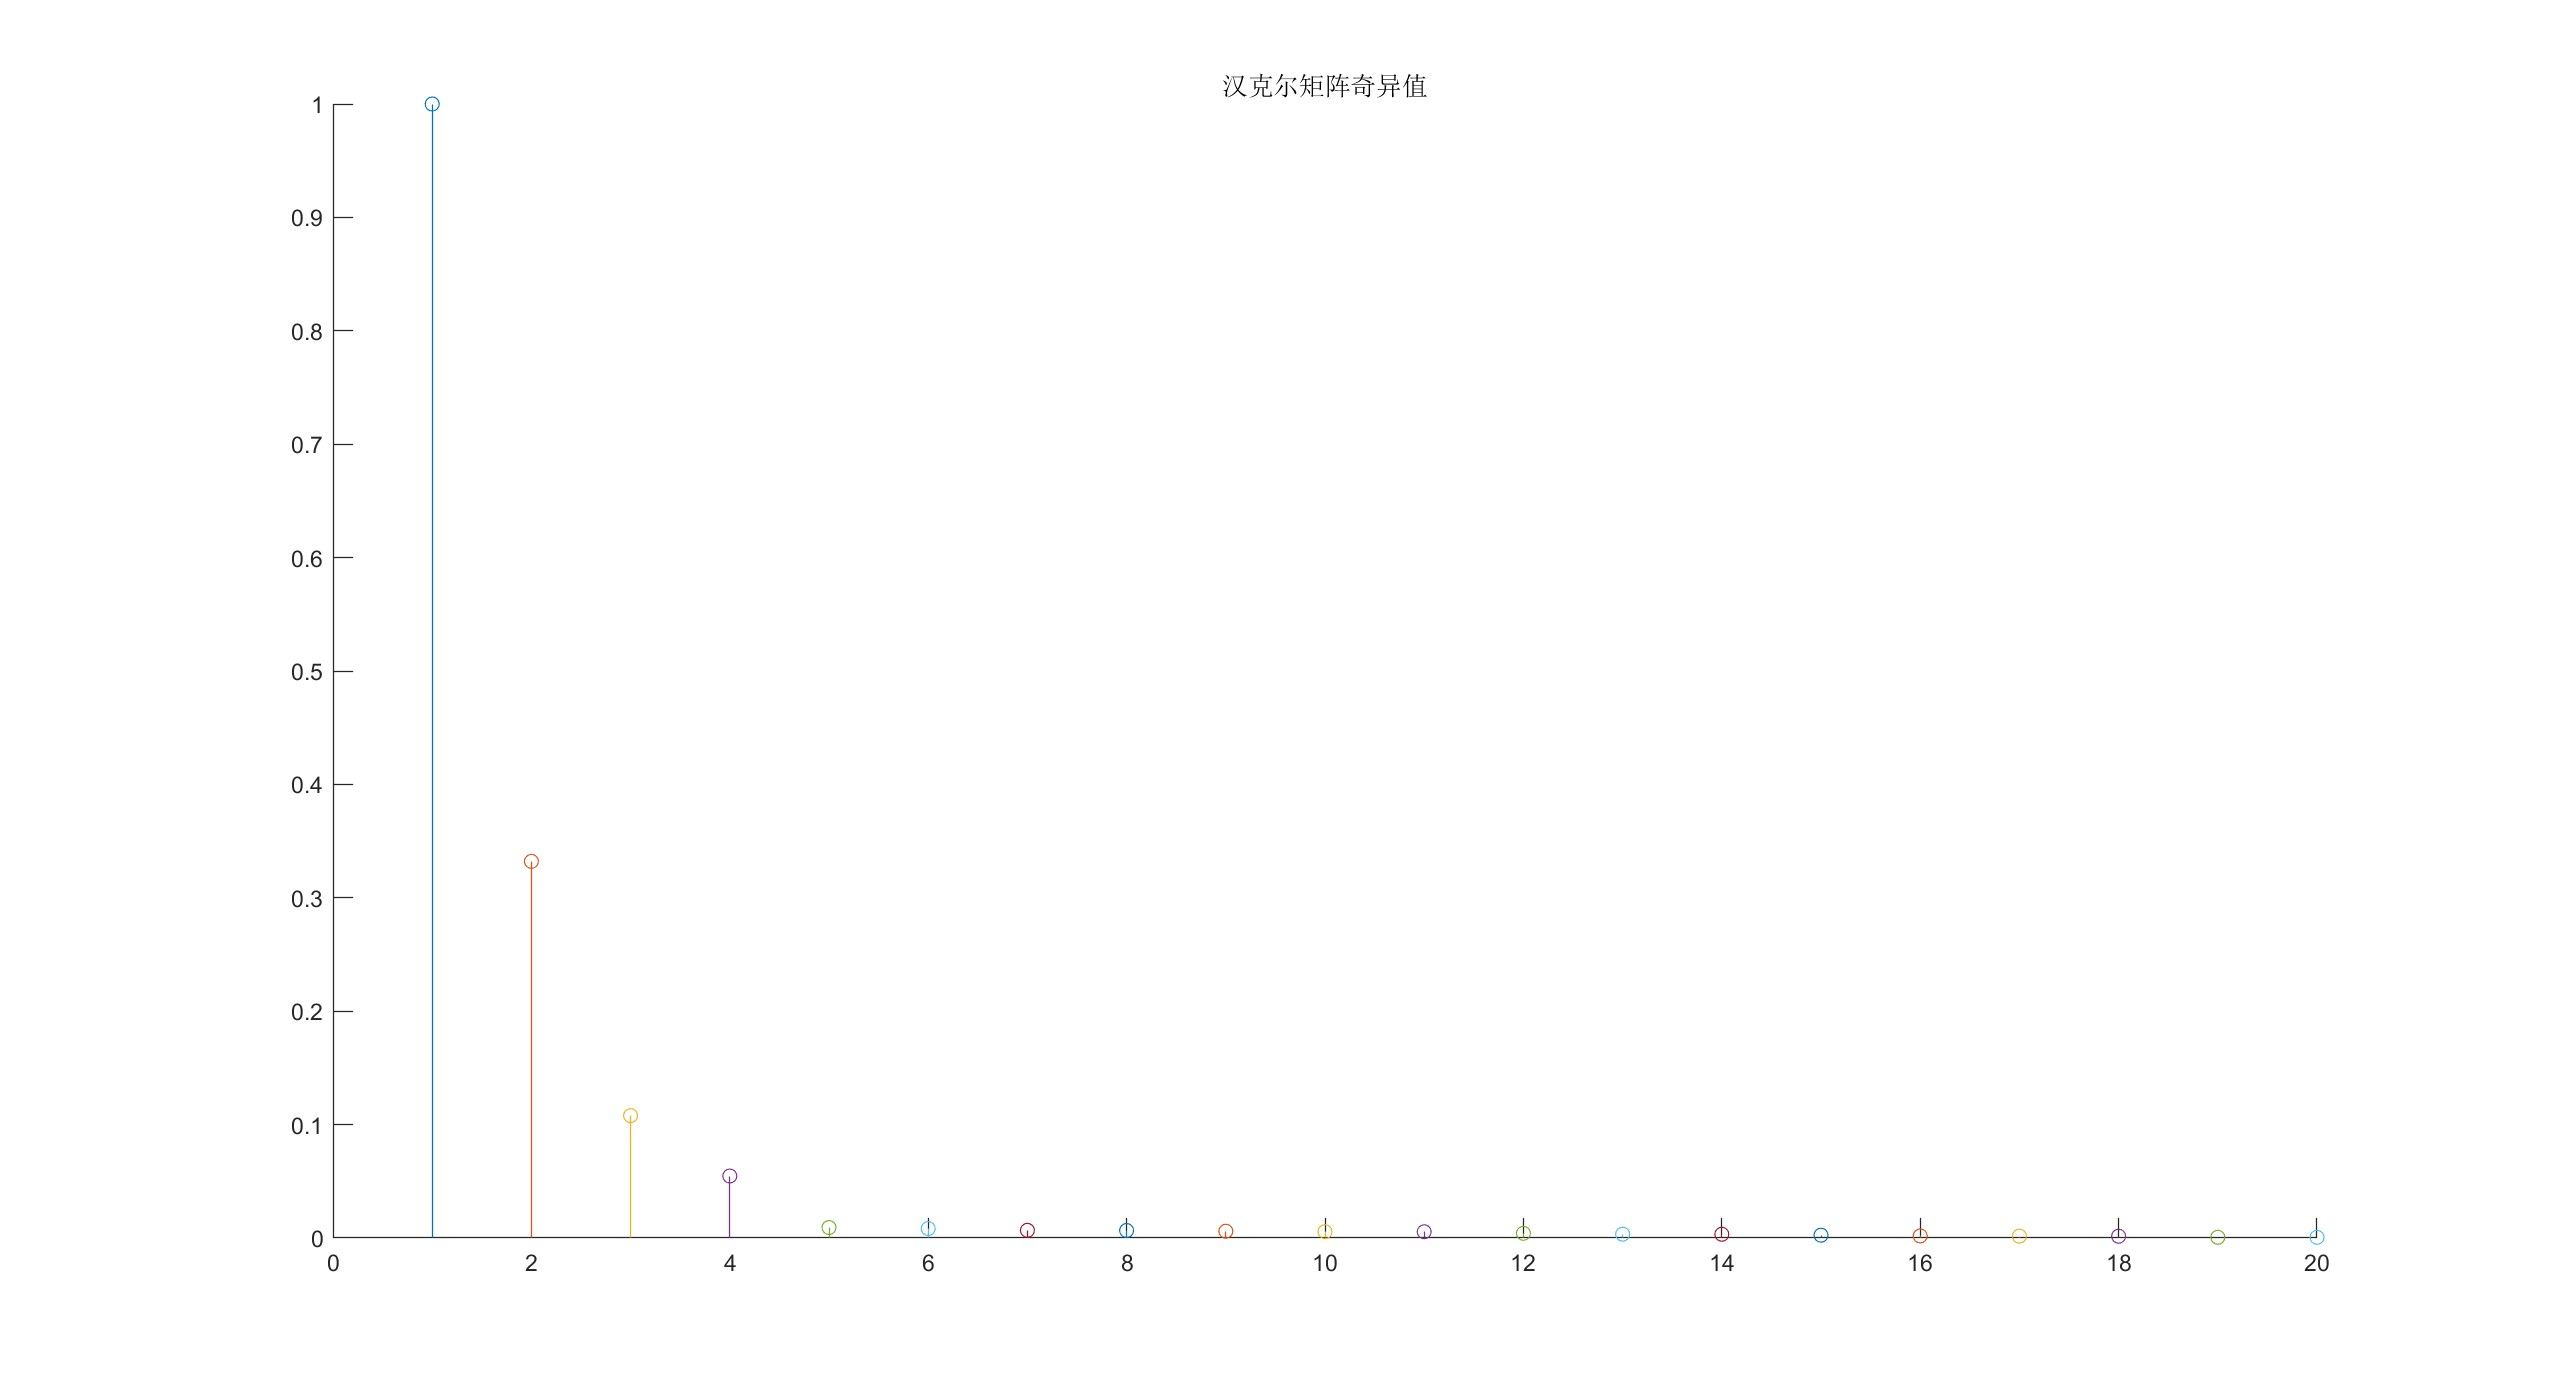
\includegraphics[width=\textwidth]
        {图片/机械堵转奇异值分解图.jpg}
        \caption{机械堵转奇异值分解图}
    \end{minipage}
    \begin{minipage}{0.5\textwidth}
        \centering
        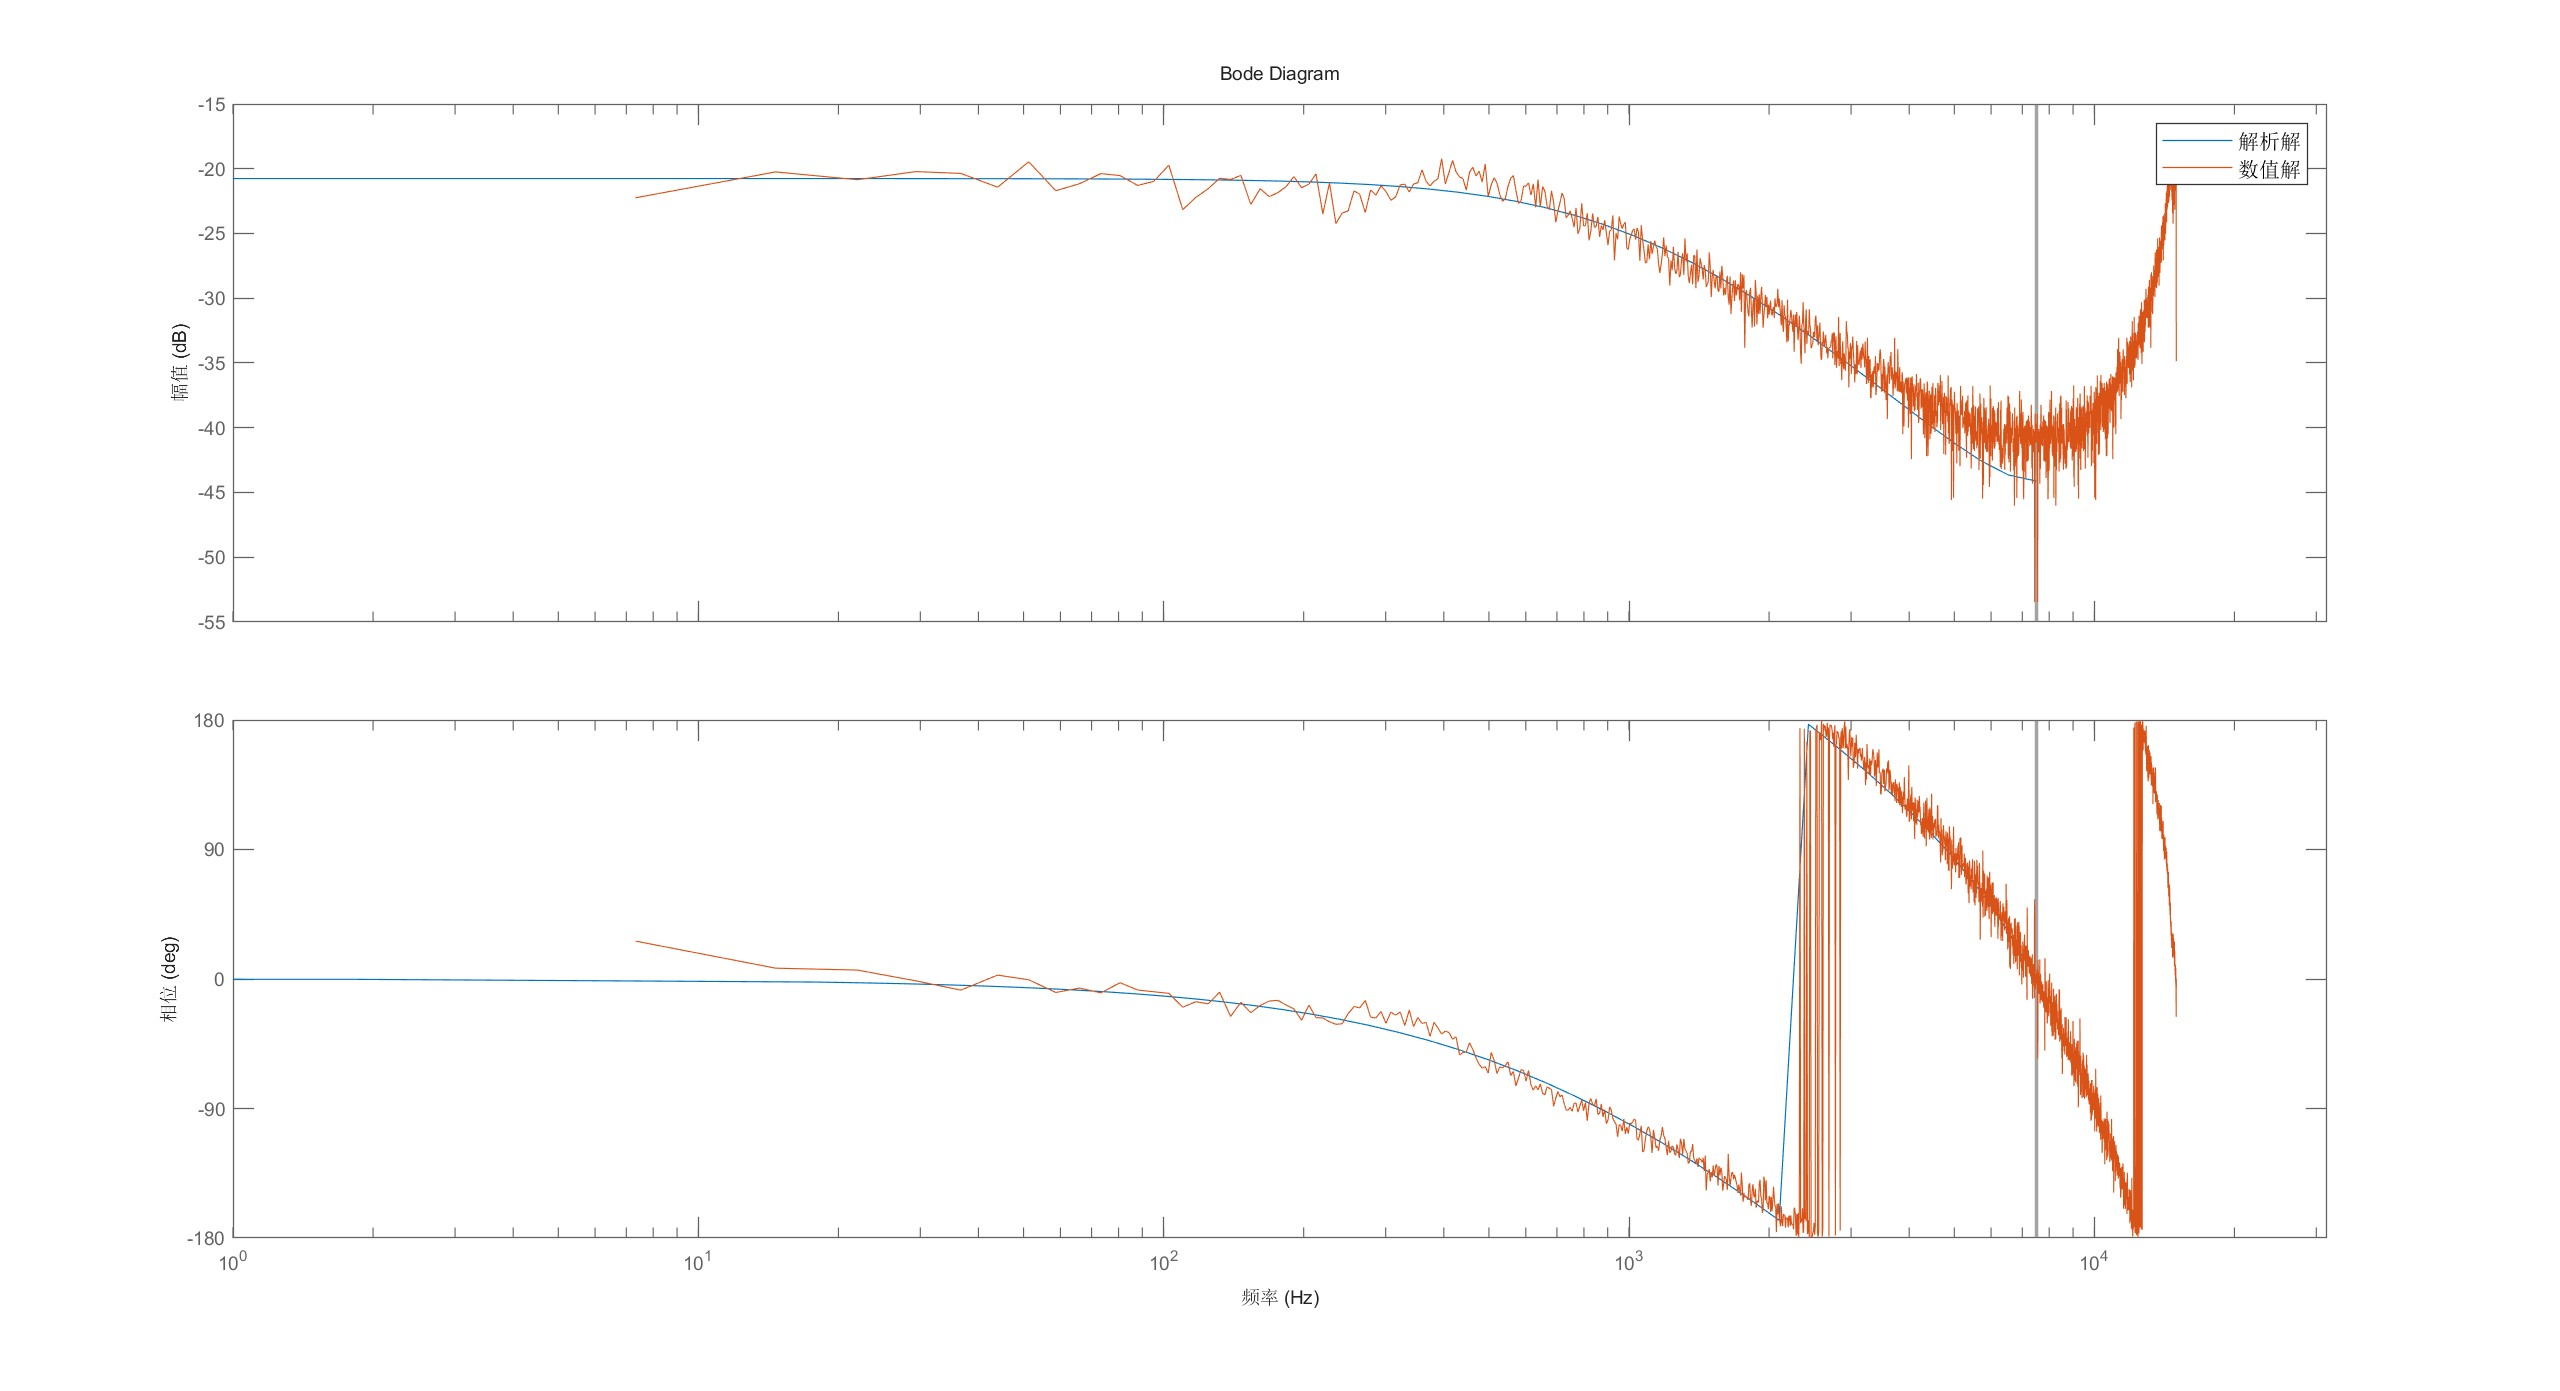
\includegraphics[width=\textwidth]
        {图片/机械堵转数值解与解析解对比.jpg}
        \caption{机械堵转数值解与解析解对比}
    \end{minipage}
\end{figure}

根据奇异值分解图，对比电气锁轴方式，可以发现系统阶次近似为二阶，转动耦合模态含量大大降低。传递函数辨识结果为
\(G(z)=\cfrac{-0.0000543  - 0.0002405 z^{-1} + 0.02709z^{-2}}{1 - 0.8149 z^{-1} + 0.0004799z^{-2}}\)，两个极点为
0.8143和0.0006。得到机械堵转下Q轴同步电感为\(L_q=1.85019\textrm{mH}\)。

上述结果看似合理，但是违背了电机的基本原理。根据D轴电感辨识结果\(L_{dO}=1.86152\textrm{mH}\)，结合相间电感估计Q轴同步电感范围
为\(L_q\in(2.13252,2.27211)\textrm{\textrm{mH}}\)，
Q轴电感需要满足\(L_q\ge 2.1\textrm{mH}\)，但是辨识结果为
\(L_{qO}\approx 1.86\textrm{mH}<2.1\textrm{mH}\)，认为是电机微动导致转动耦合模态没有完全消失，
而是和RL电路的模态融合成了一个极点，导致Q轴电感辨识不准确。

\subsubsection{数据后处理方法}
机械堵转和电气堵转都难以抵消运动模态带来的影响，最终选择后期数据处理。

通过后期补偿，在工作点0V附近进行HK辨识结果如下。可以发现，脉冲响应序列不再出现振荡。
\begin{figure}[H]
    \centering
    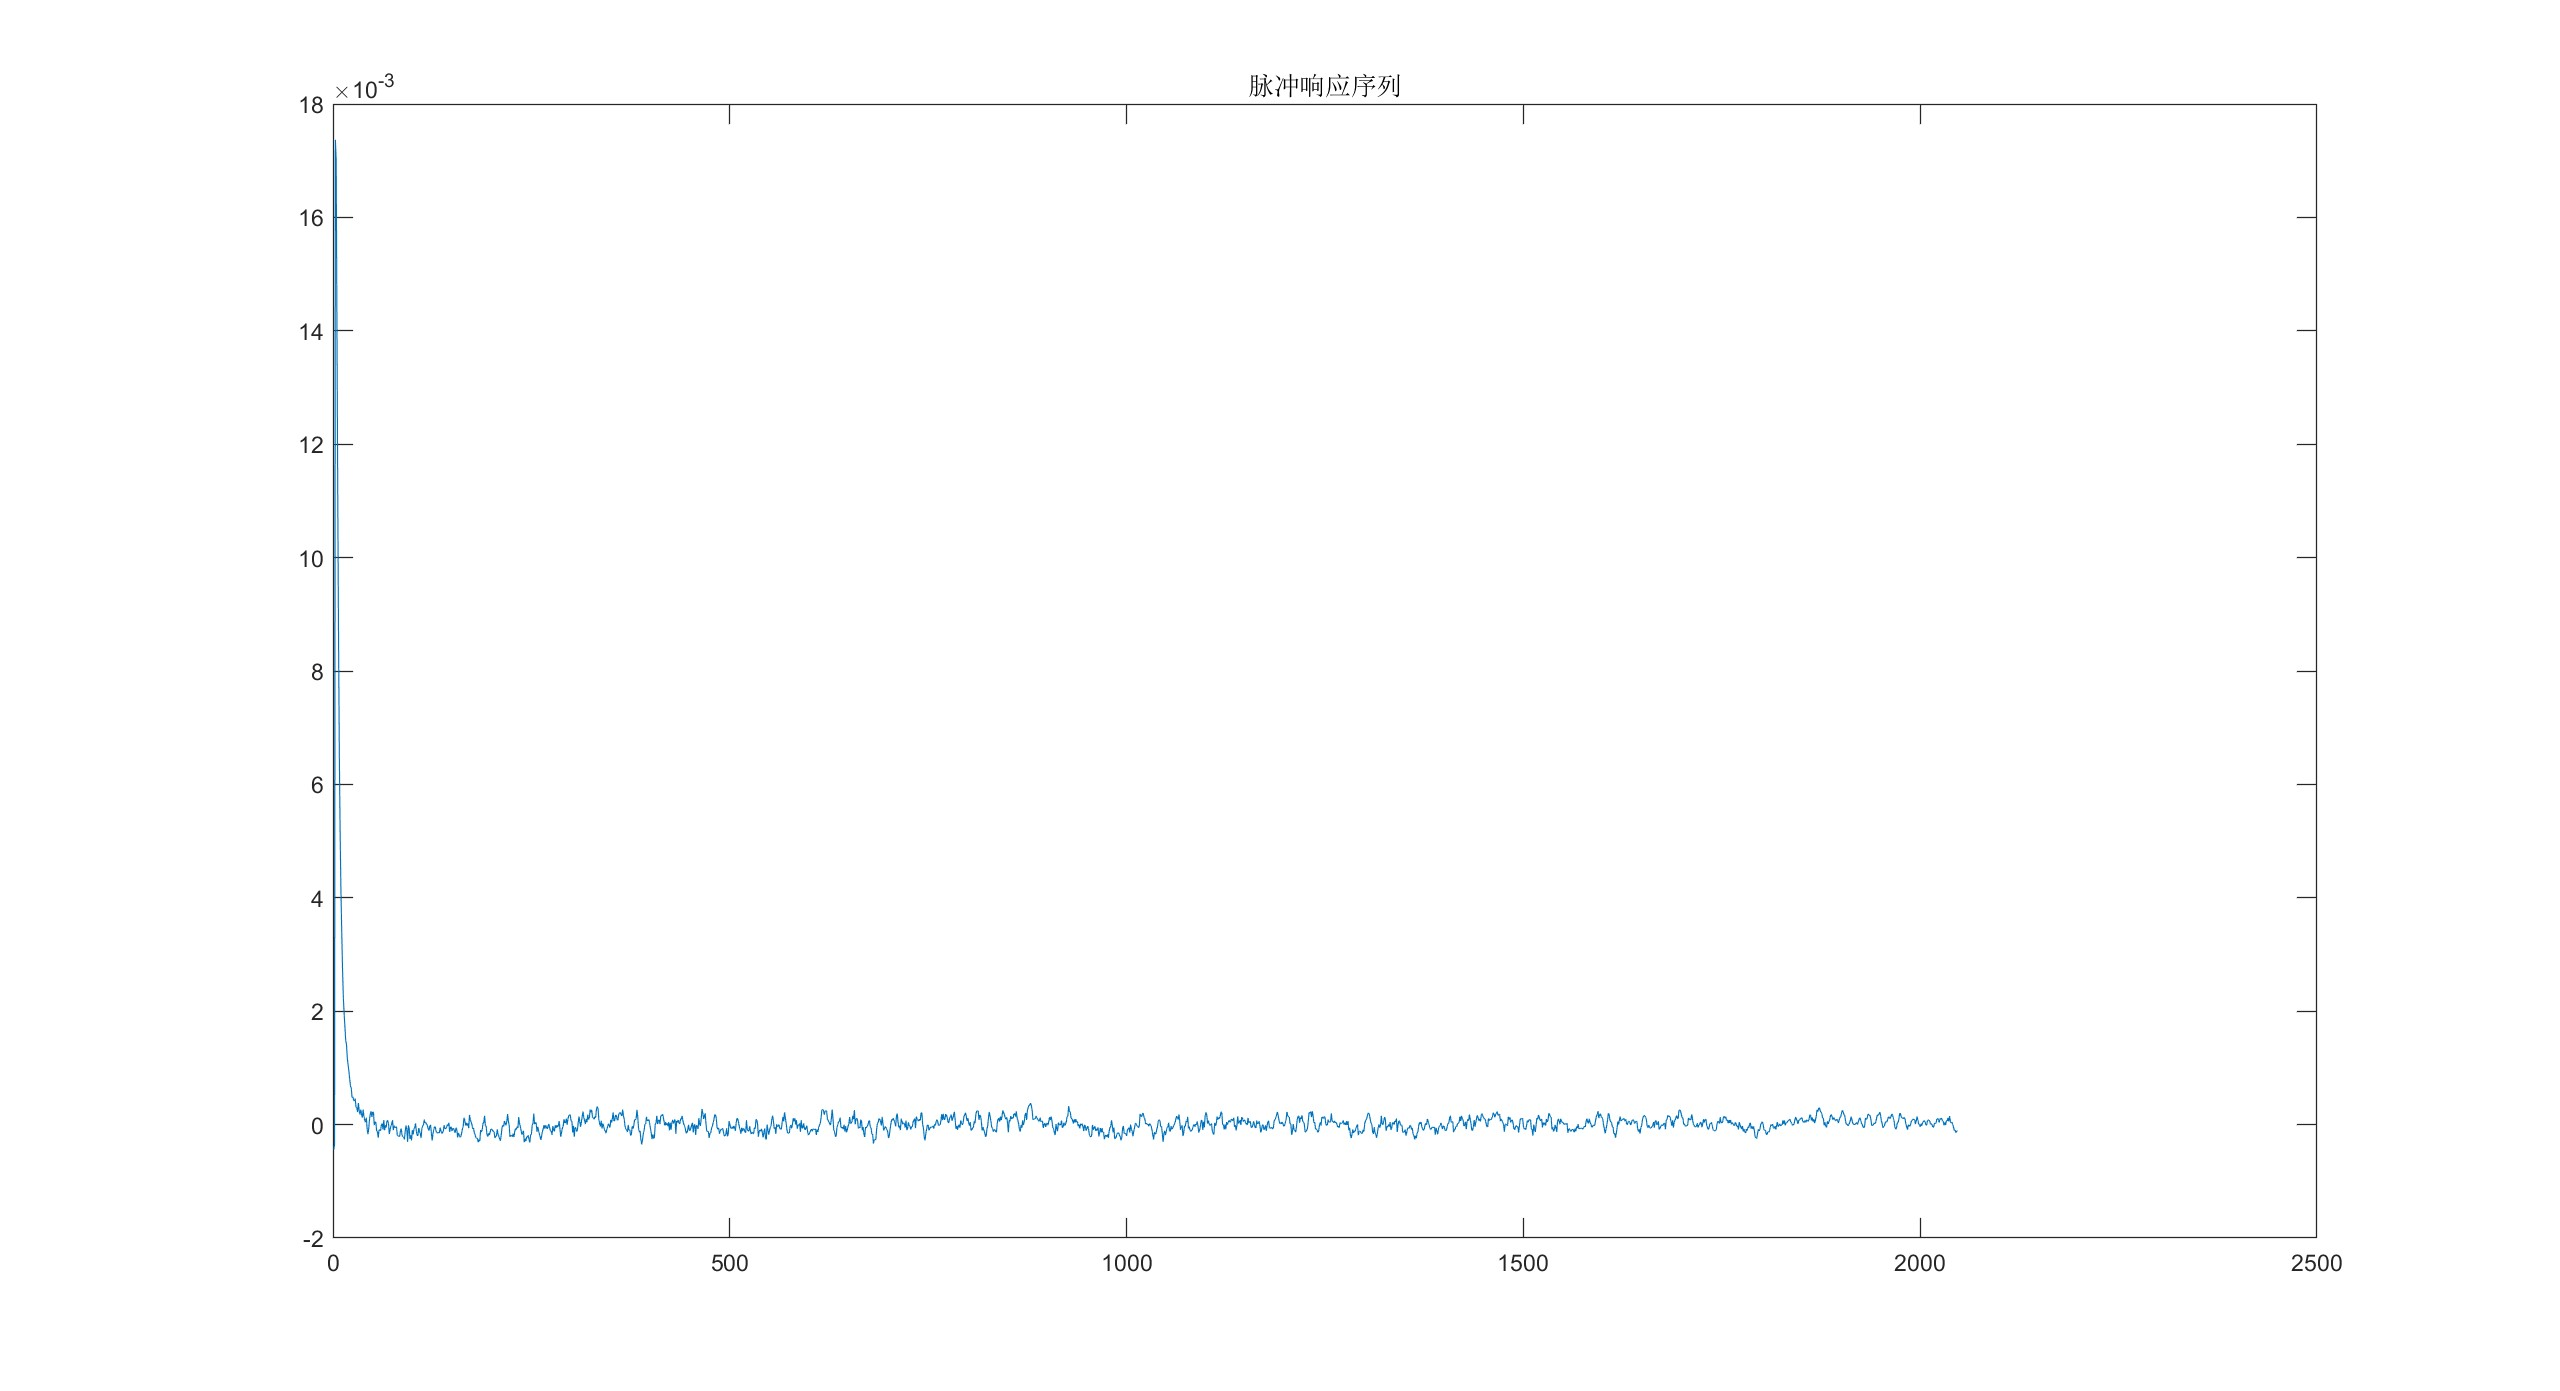
\includegraphics[width=0.5\textwidth]
    {图片/Q轴工作点0V脉冲响应序列.jpg}
    \caption{Q轴工作点0V脉冲响应序列}
\end{figure}

奇异值分解图和数值解解析解对比如下图所示。数值解与解析解的幅频相关系数为99.50080\(\%\)，
相频相关系数为99.97588\(\%\)，拟合优度90.81283\(\%\)。解析解传递函数为
\(G(z)=\cfrac{-0.000036  - 0.000101 z^{-1} + 0.0267z^{-2}}{1 - 0.8013 z^{-1} - 0.03188z^{-2}}\)，两个极点为
0.8393和-0.038。选取慢极点0.8393，根据\(L_q=-\cfrac{R_sT_s}{\ln(z_p)}\)计算Q轴电感为\(L_q=2.16828\textrm{mH}\)。
该辨识结果满足\(L_q\ge L_d\)，并且也满足相间电感估测结果\(L_q\in(2.13252,2.27211)\textrm{\textrm{mH}}\)。
\begin{figure}[H]
    \begin{minipage}{0.5\textwidth}
        \centering
        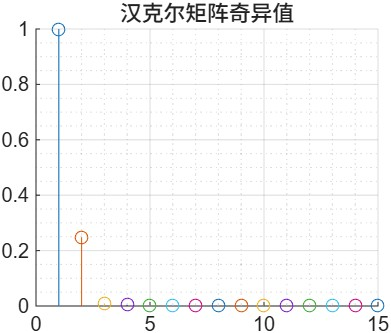
\includegraphics[width=\textwidth]
        {图片/Q轴工作点0V奇异值分解图.jpg}
        \caption{Q轴工作点0V奇异值分解图}
    \end{minipage}
    \begin{minipage}{0.5\textwidth}
        \centering
        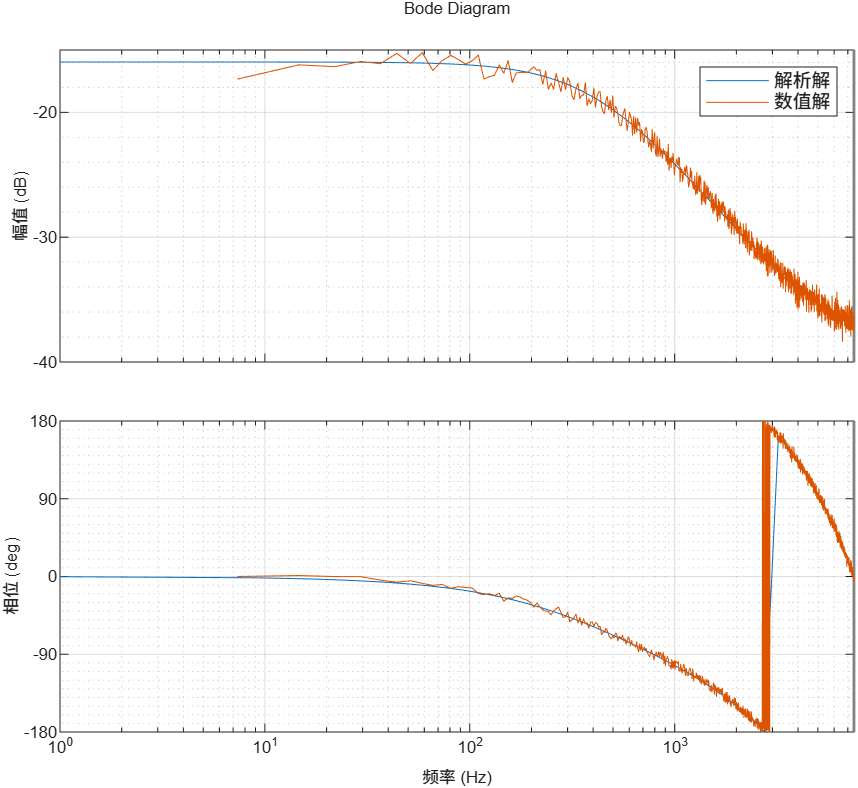
\includegraphics[width=\textwidth]
        {图片/Q轴工作点0V数值解和解析解对比.jpg}
        \caption{Q轴工作点0V数值解和解析解对比}
    \end{minipage}
\end{figure}

按照相同的方法，对工作点\(\pm2\)V、\(\pm4\)V进行辨识，结果如下。

工作点2V时，得到的Hankel矩阵奇异值分解和频域响应对比如下图所示。数值解与解析解的幅频相关系数为98.99637\(\%\)，
相频相关系数为99.95608\(\%\)，拟合优度84.70566\(\%\)。解析解传递函数为
\(G(z)=\cfrac{-0.0003126  - 0.0001889 z^{-1} + 0.02554z^{-2}}{1 - 0.8179 z^{-1} - 0.01559z^{-2}}\)，两个极点为
0.8365和-0.0186。得到2V工作点下Q轴同步电感为\(L_q=2.12868\textrm{mH}\)。
\begin{figure}[H]
    \begin{minipage}{0.5\textwidth}
        \centering
        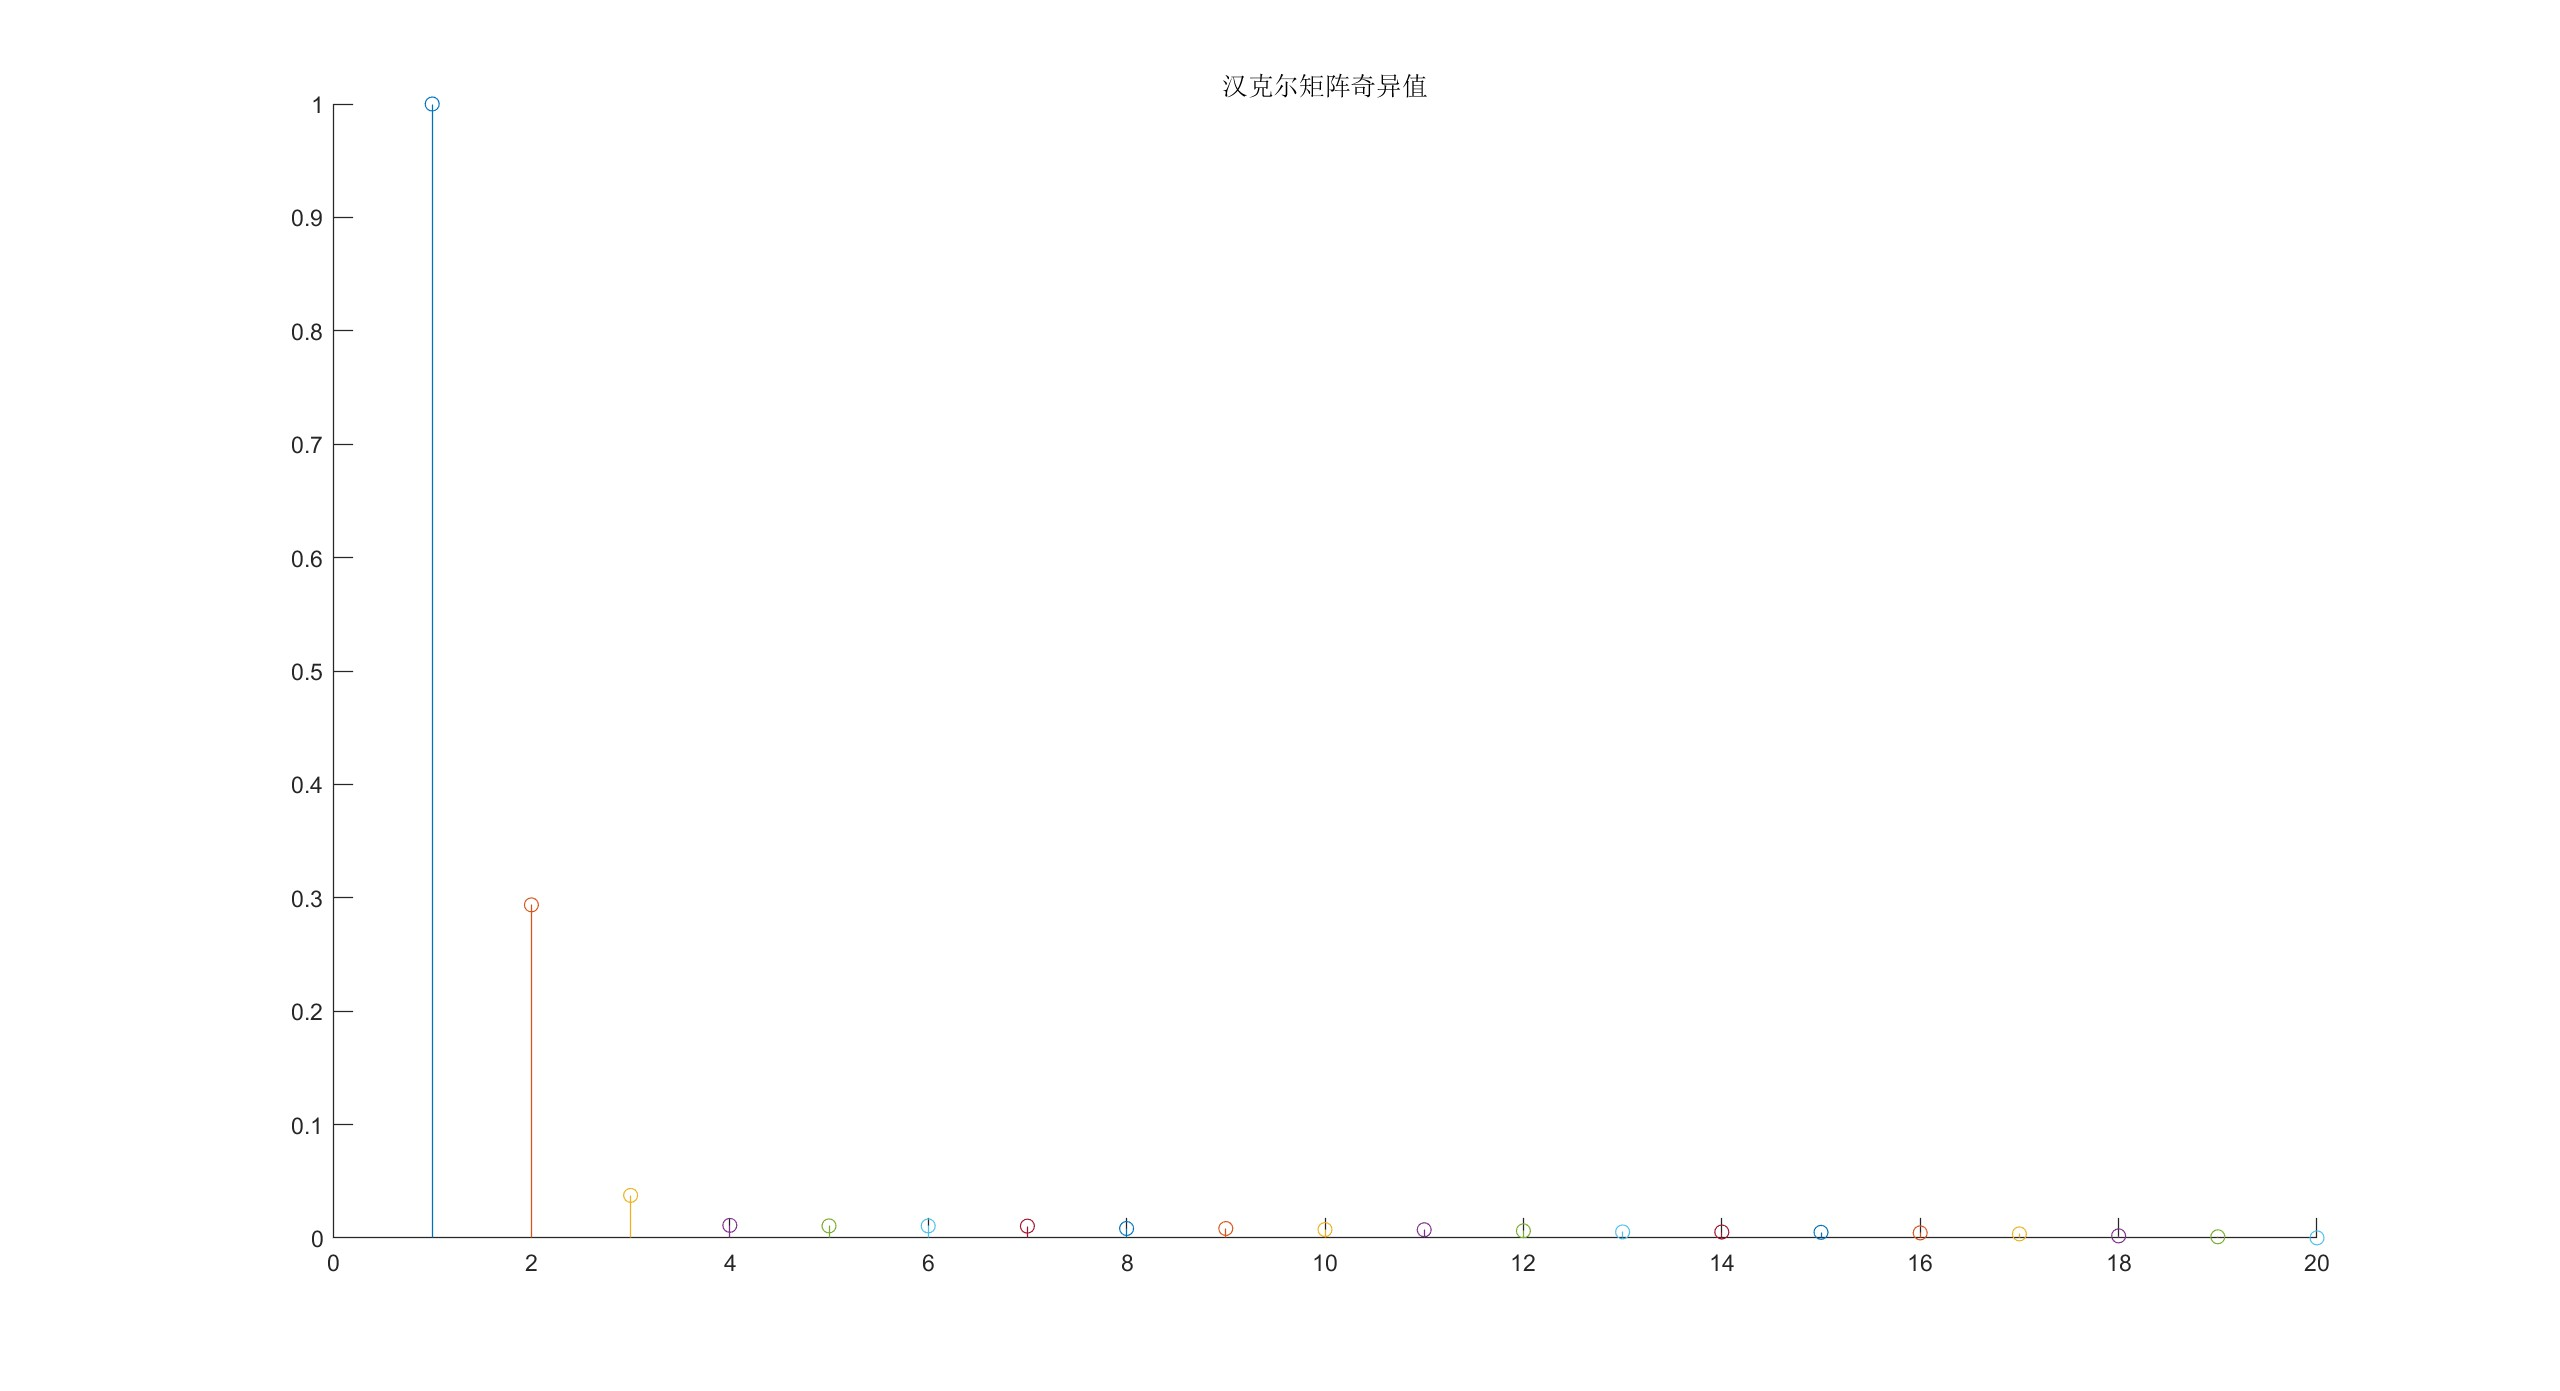
\includegraphics[width=\textwidth]
        {图片/Q轴工作点2V奇异值分解图.jpg}
        \caption{Q轴工作点2V奇异值分解图}
    \end{minipage}
    \begin{minipage}{0.5\textwidth}
        \centering
        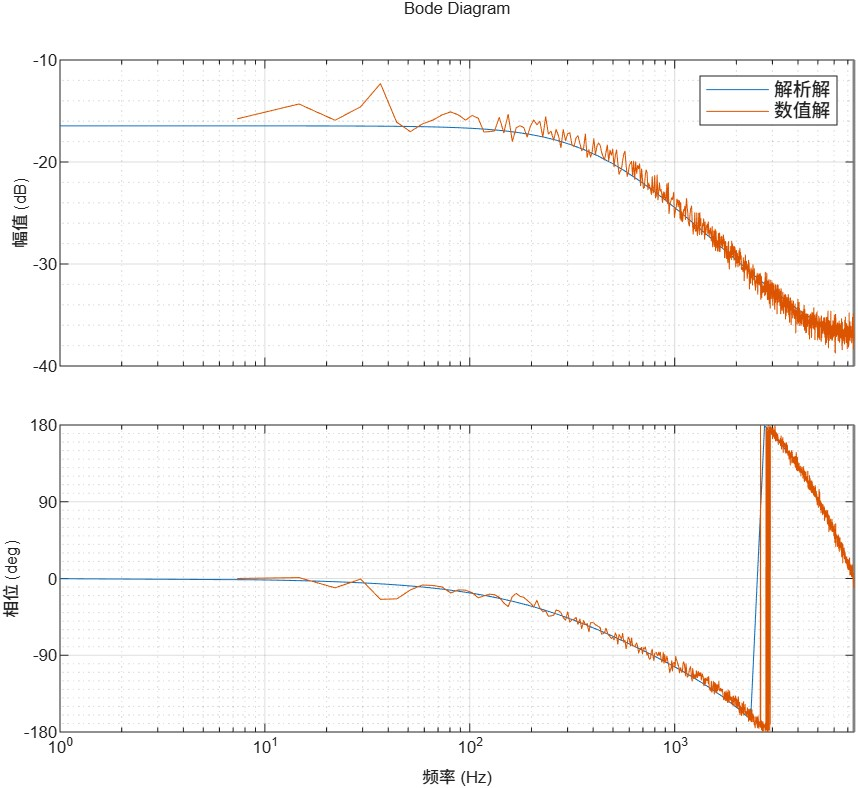
\includegraphics[width=\textwidth]
        {图片/Q轴工作点2V数值解和解析解对比.jpg}
        \caption{Q轴工作点2V数值解和解析解对比}
    \end{minipage}
\end{figure}

工作点4V时，得到的Hankel矩阵奇异值分解和频域响应对比如下图所示。数值解与解析解的幅频相关系数为98.65486\(\%\)，
相频相关系数为99.94388\(\%\)，拟合优度82.84616\(\%\)。解析解传递函数为
\(G(z)=\cfrac{-0.0003139  + 0.0001031 z^{-1} + 0.02462z^{-2}}{1 - 0.837 z^{-1} - 0.004508z^{-2}}\)，两个极点为
0.8424和-0.0054。得到4V工作点下Q轴同步电感为\(L_q=2.21481\textrm{mH}\)。
\begin{figure}[H]
    \begin{minipage}{0.5\textwidth}
        \centering
        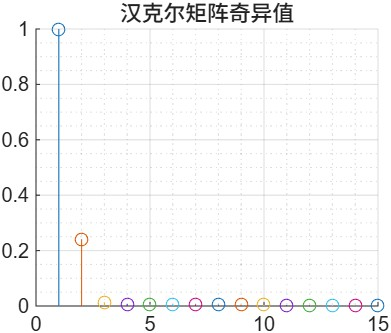
\includegraphics[width=\textwidth]
        {图片/Q轴工作点4V奇异值分解图.jpg}
        \caption{Q轴工作点4V奇异值分解图}
    \end{minipage}
    \begin{minipage}{0.5\textwidth}
        \centering
        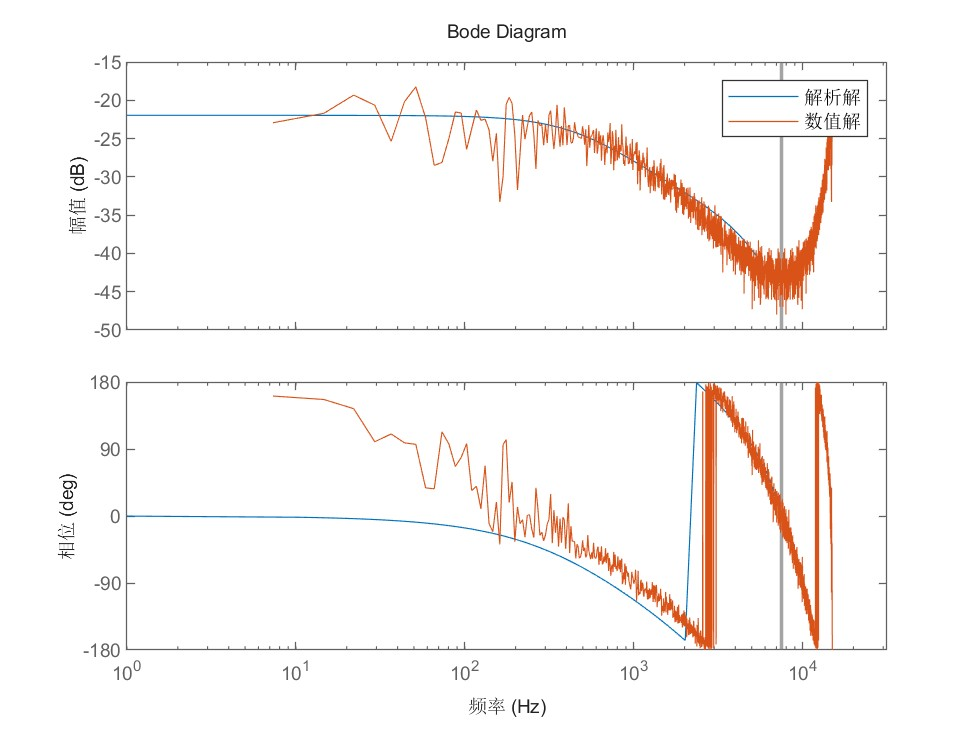
\includegraphics[width=\textwidth]
        {图片/Q轴工作点4V数值解和解析解对比.jpg}
        \caption{Q轴工作点4V数值解和解析解对比}
    \end{minipage}
\end{figure}

工作点-2V时，得到的Hankel矩阵奇异值分解和频域响应对比如下图所示。数值解与解析解的幅频相关系数为99.00722\(\%\)，
相频相关系数为99.97406\(\%\)，拟合优度86.66177\(\%\)。解析解传递函数为
\(G(z)=\cfrac{-0.00007114  + 0.00005972 z^{-1} + 0.02562z^{-2}}{1 - 0.8119 z^{-1} - 0.0271z^{-2}}\)，两个极点为
0.8440和-0.0321。得到-2V工作点下Q轴同步电感为\(L_q=2.24055\textrm{mH}\)。
\begin{figure}[H]
    \begin{minipage}{0.5\textwidth}
        \centering
        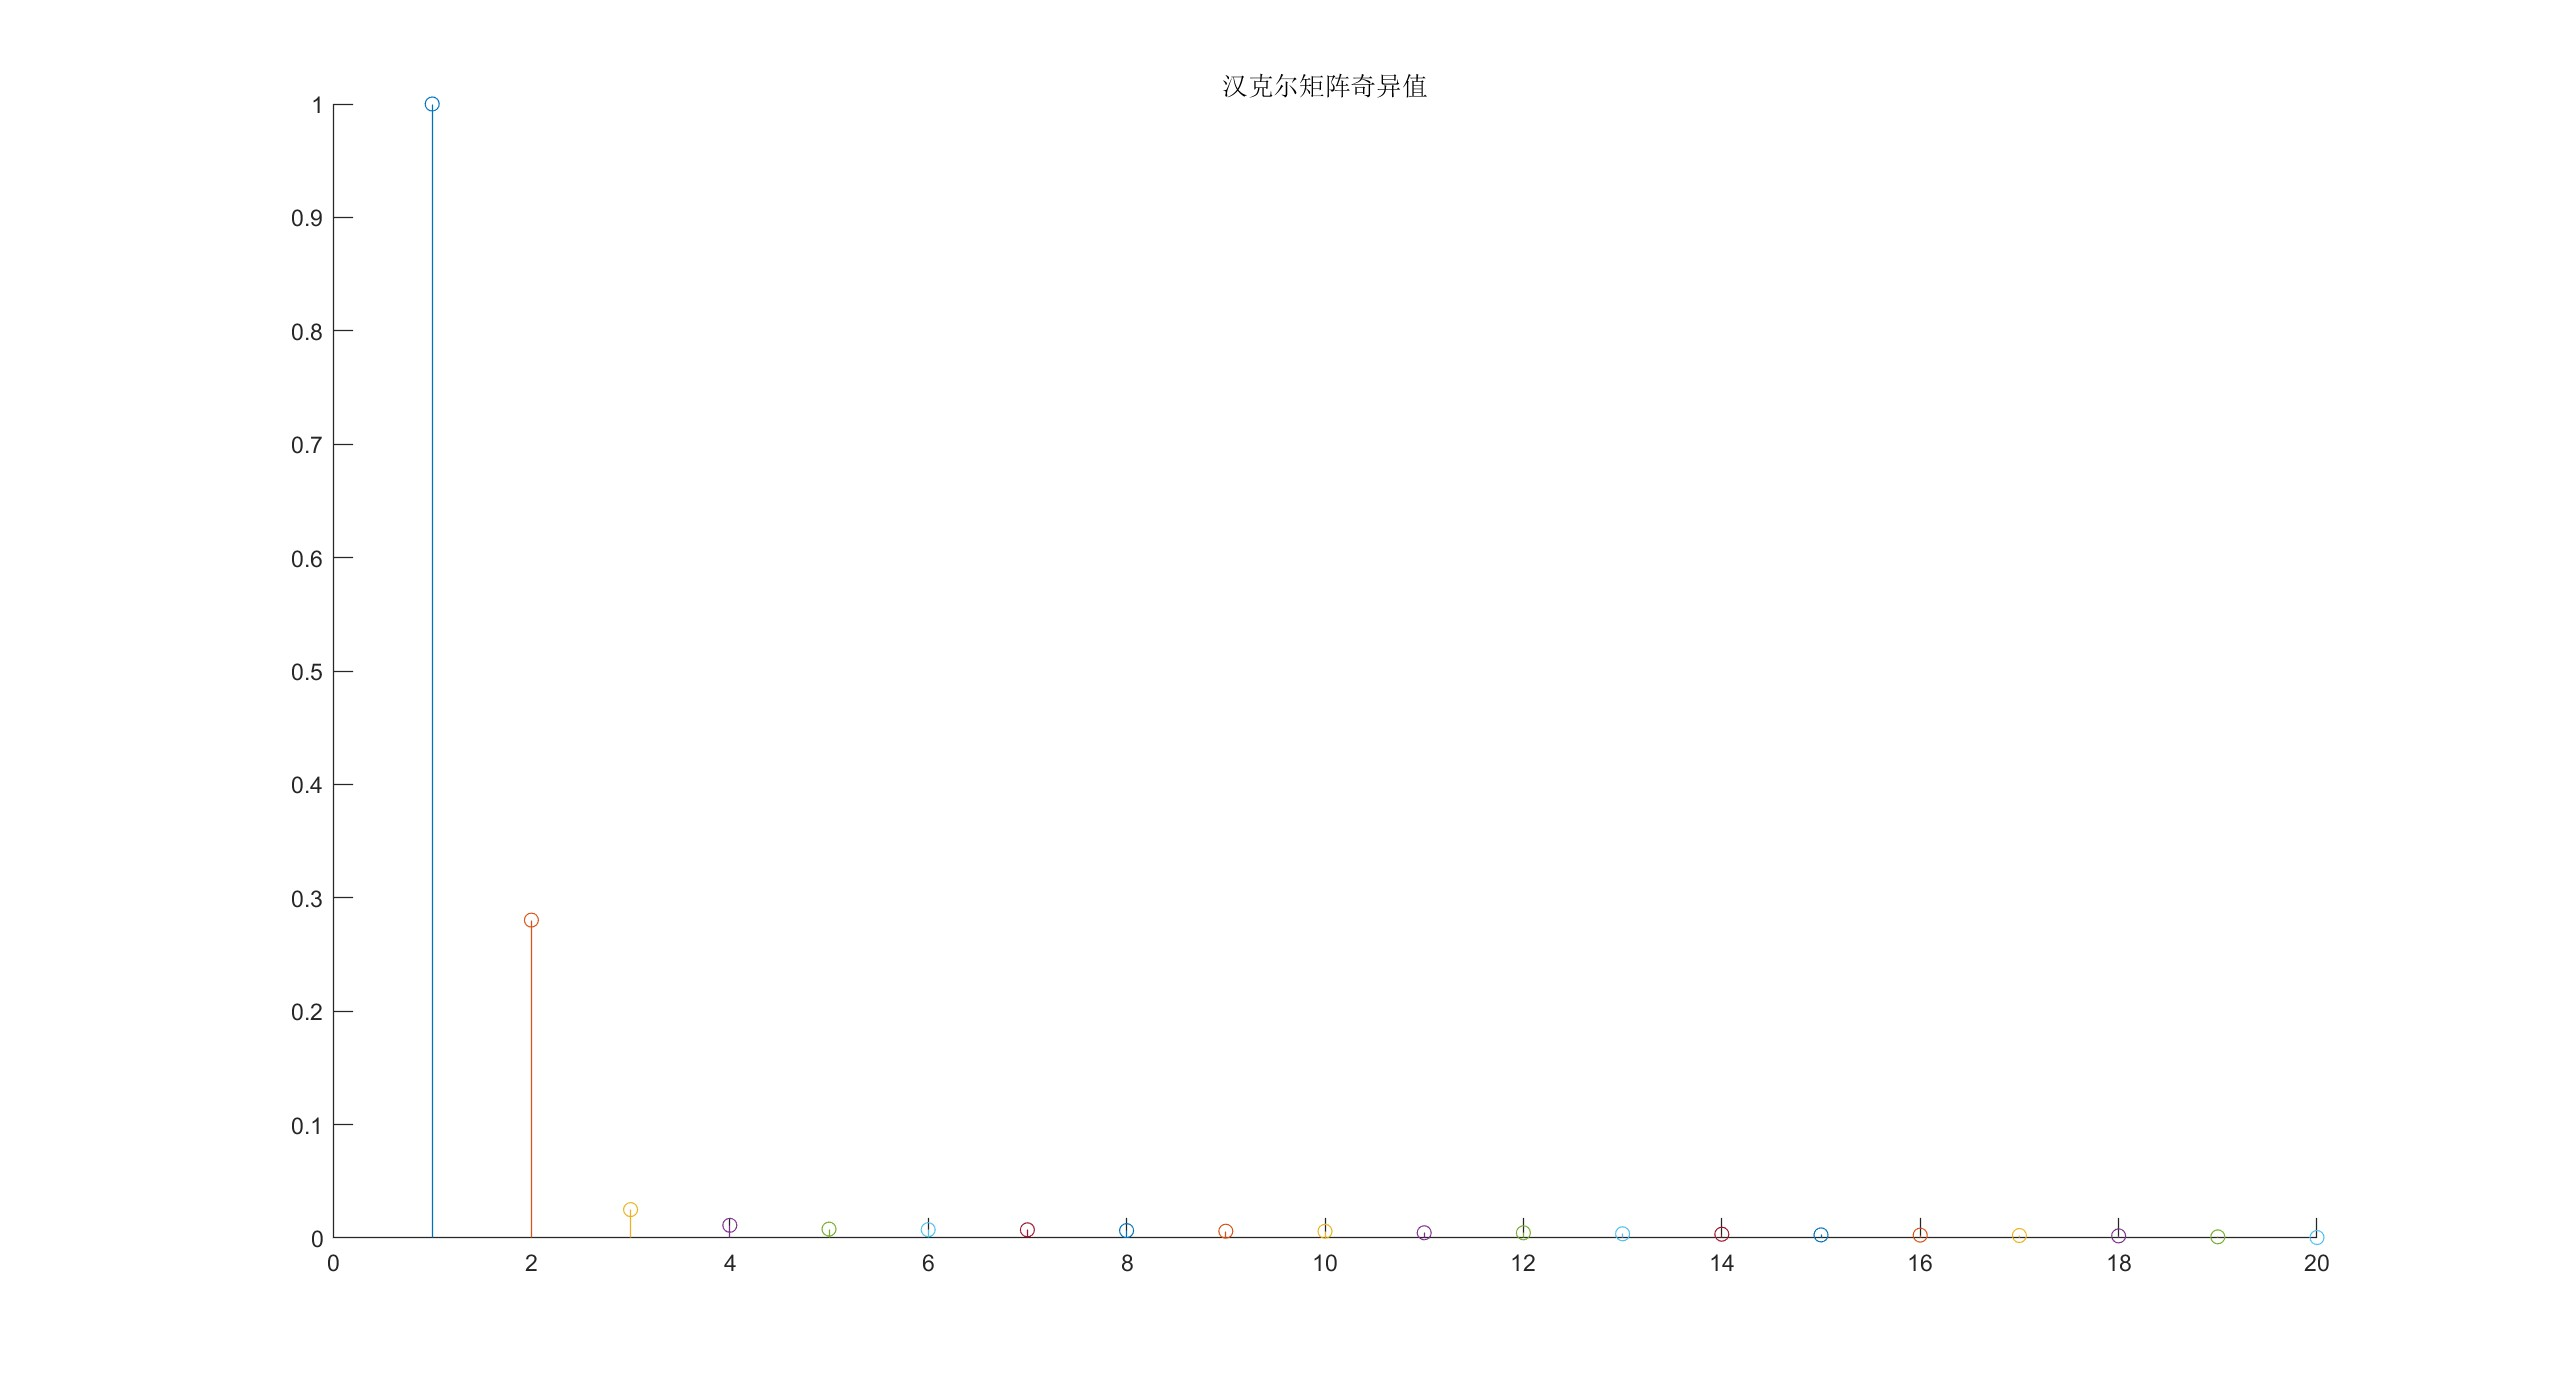
\includegraphics[width=\textwidth]
        {图片/Q轴工作点-2V奇异值分解图.jpg}
        \caption{Q轴工作点-2V奇异值分解图}
    \end{minipage}
    \begin{minipage}{0.5\textwidth}
        \centering
        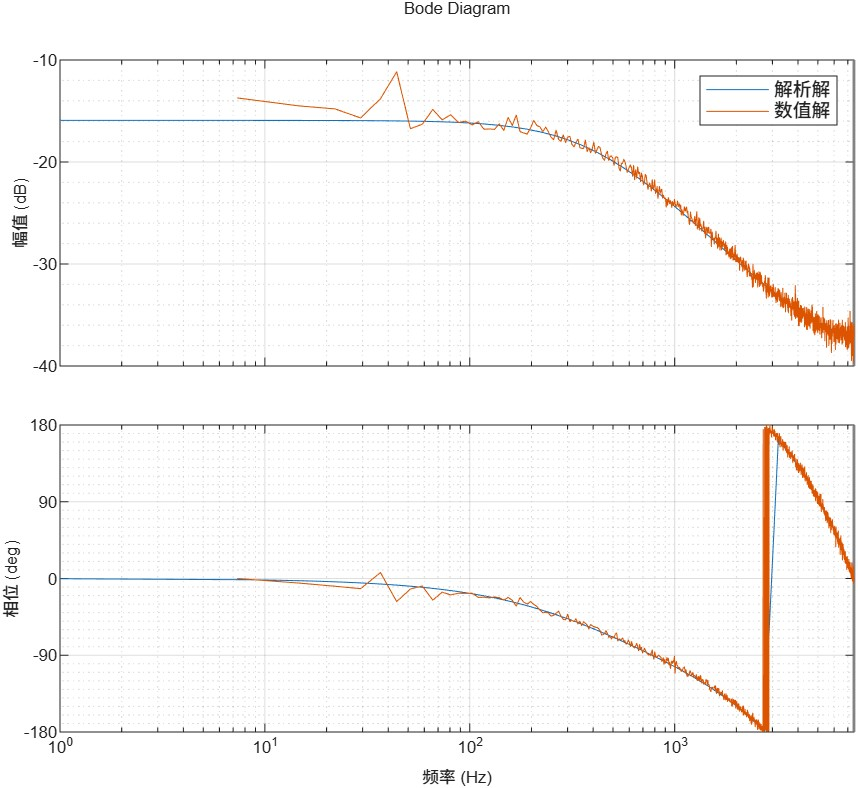
\includegraphics[width=\textwidth]
        {图片/Q轴工作点-2V数值解和解析解对比.jpg}
        \caption{Q轴工作点-2V数值解和解析解对比}
    \end{minipage}
\end{figure}

工作点-4V时，得到的Hankel矩阵奇异值分解和频域响应对比如下图所示。数值解与解析解的幅频相关系数为99.24784\(\%\)，
相频相关系数为99.96070\(\%\)，拟合优度86.58094\(\%\)。解析解传递函数为
\(G(z)=\cfrac{-0.00003683 - 0.0002048 z^{-1} + 0.02451z^{-2}}{1 - 0.8267 z^{-1} - 0.01035z^{-2}}\)，两个极点为
0.8309和-0.0123。得到-4V工作点下Q轴同步电感为\(L_q=2.16473\textrm{mH}\)。
\begin{figure}[H]
    \begin{minipage}{0.5\textwidth}
        \centering
        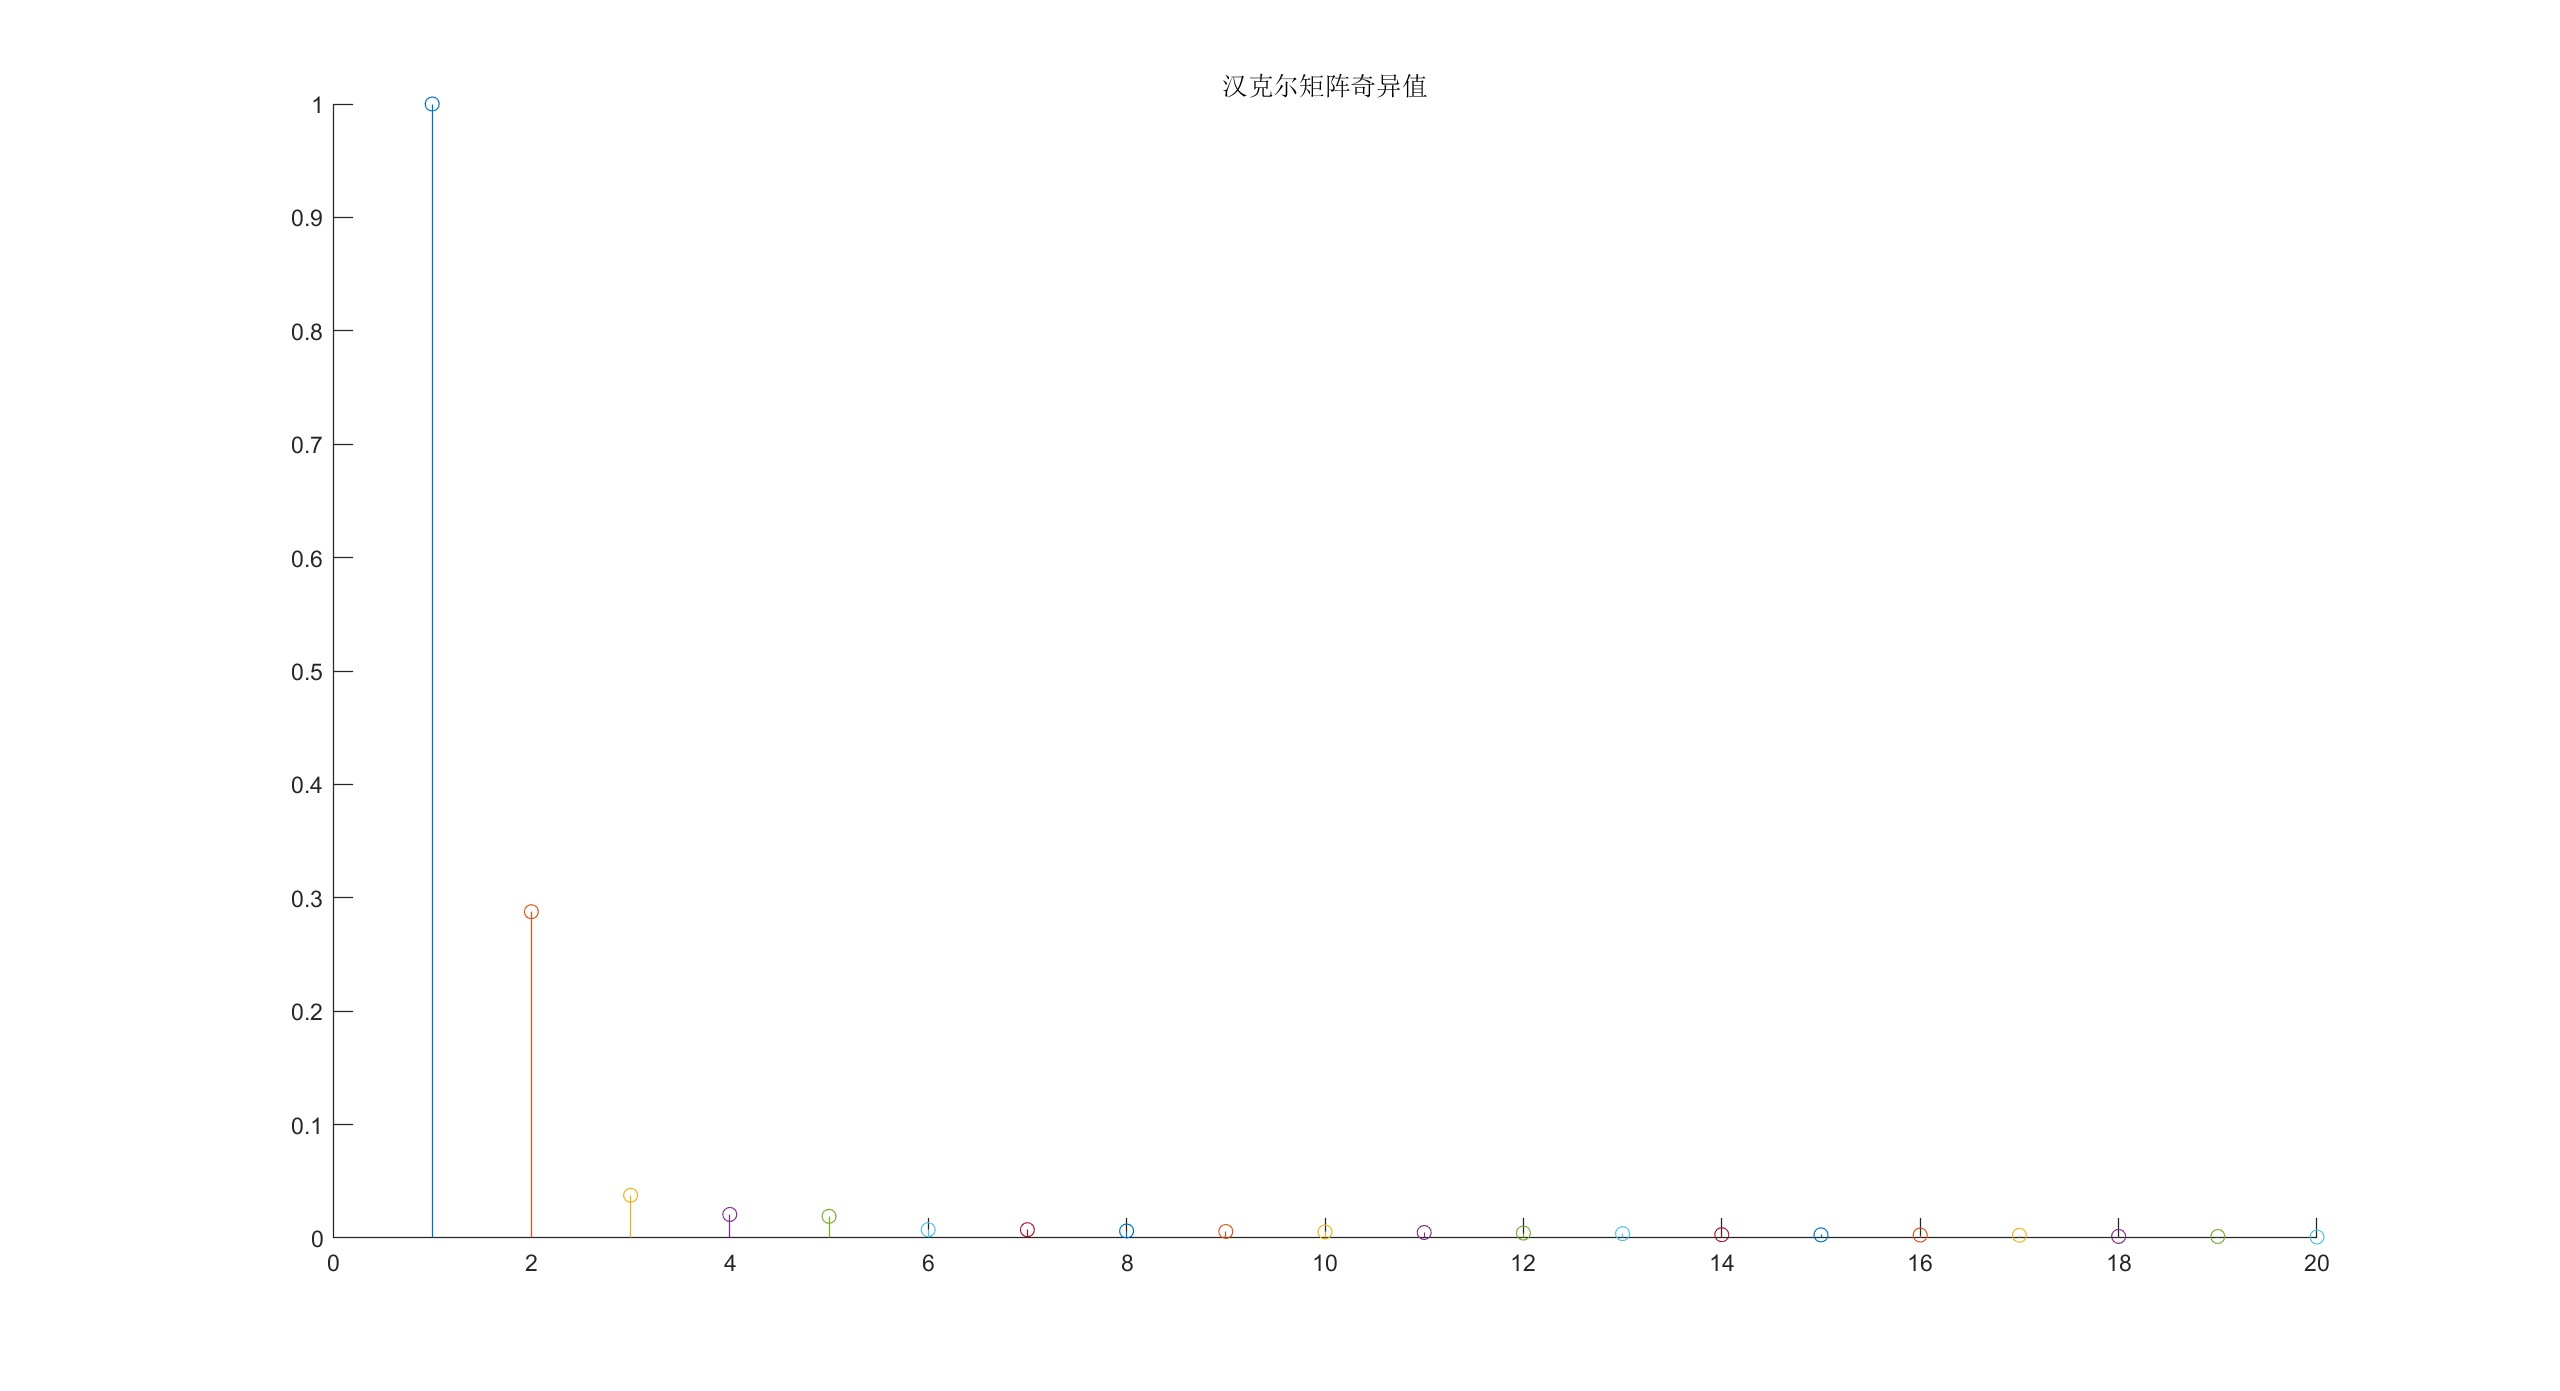
\includegraphics[width=\textwidth]
        {图片/Q轴工作点-4V奇异值分解图.jpg}
        \caption{Q轴工作点-4V奇异值分解图}
    \end{minipage}
    \begin{minipage}{0.5\textwidth}
        \centering
        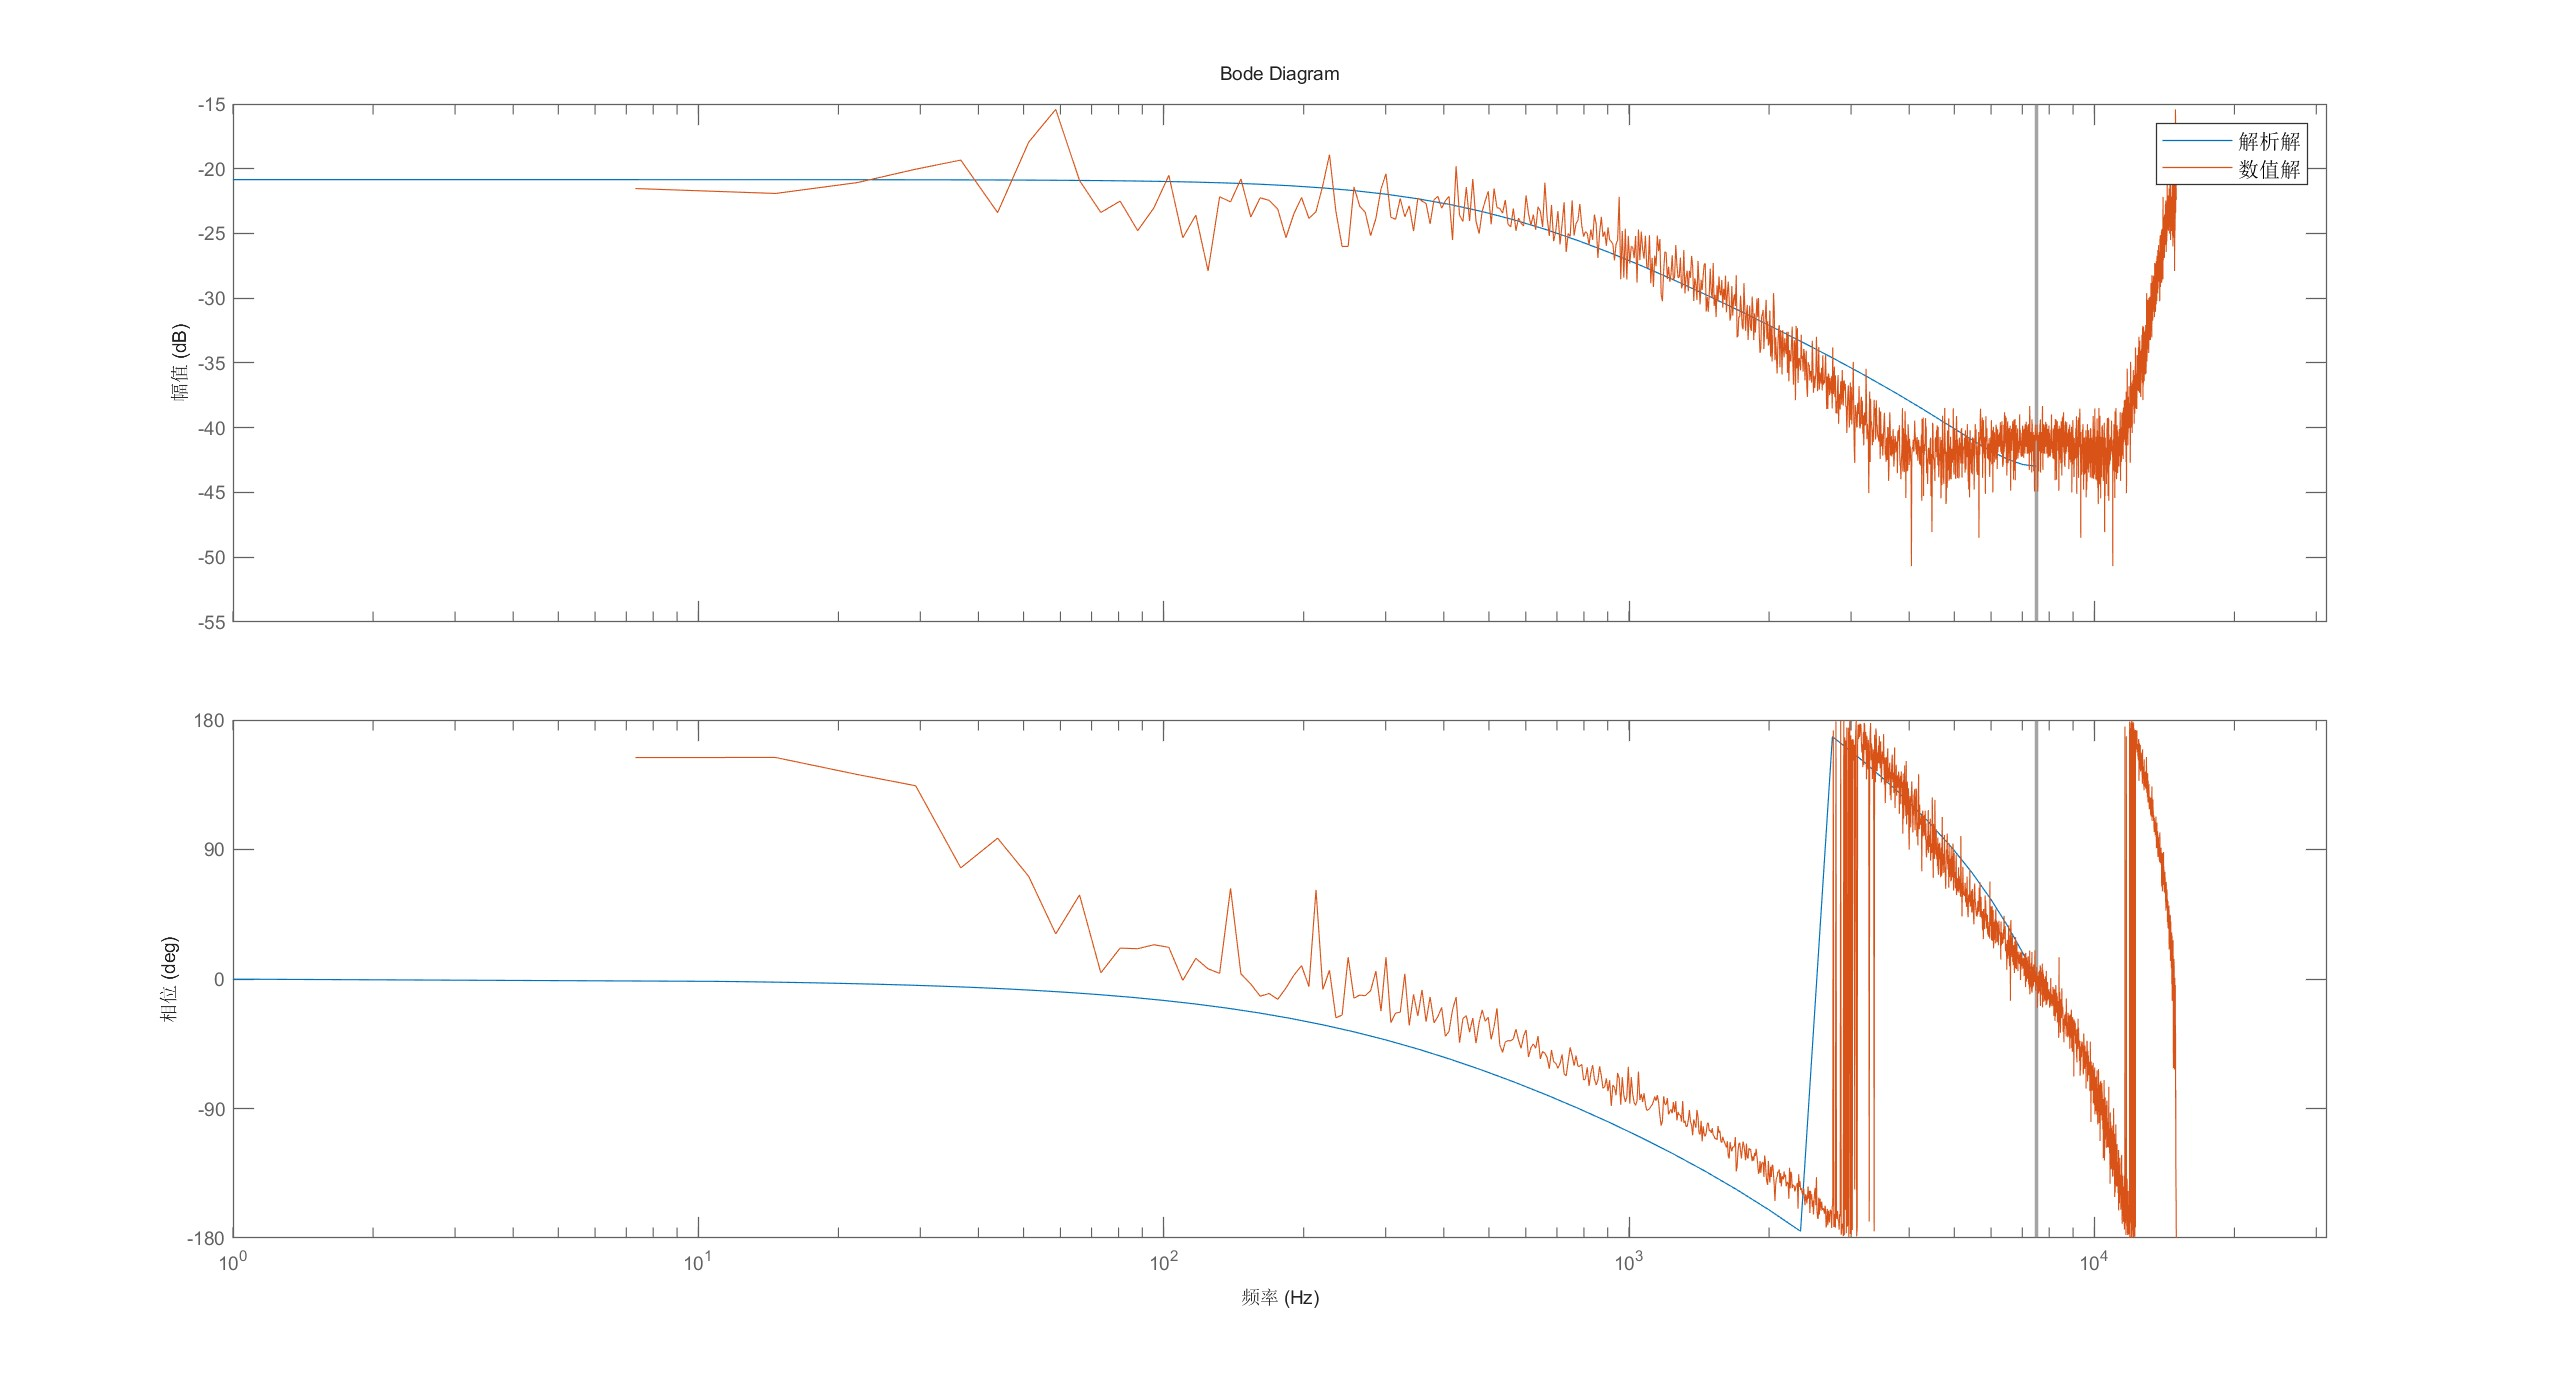
\includegraphics[width=\textwidth]
        {图片/Q轴工作点-4V数值解和解析解对比.jpg}
        \caption{Q轴工作点-4V数值解和解析解对比}
    \end{minipage}
\end{figure}

将上述五个工作点的Q轴辨识结果汇总如下表所示。
\begin{table}[H]
    \centering
    \begin{tabular}{|c|c|c|c|c|}
        \hline
        工作点 & 幅频相关系数 & 相频相关系数 & 拟合优度 & \(L_q\)辨识值（mH）\\
        \hline
        \(U_q=-4\text{V}\)  & 99.24784\% & 99.96070\% & 86.58094\% & 2.16473\\
        \hline
        \(U_q=-2\text{V}\)  & 99.00722\% & 99.97406\% & 86.66177\% & 2.24055\\
        \hline
        \(U_q=0\text{V}\)   & 99.50080\% & 99.97588\% & 90.81283\% & 2.16828\\
        \hline
        \(U_q=2\text{V}\)   & 98.99637\% & 99.95608\% & 84.70566\% & 2.12868\\
        \hline
        \(U_q=4\text{V}\)   & 98.65486\% & 99.94388\% & 82.84616\% & 2.21481\\
        \hline
    \end{tabular}
    \caption{Q轴各工作点HK辨识结果汇总}
    \label{tab:Q轴各工作点辨识结果汇总}
\end{table}

可以发现，随着工作点绝对值升高，数值解与解析解的相关系数快速降低。
推测是因为随着工作点绝对值升高，转速也随之升高，齿槽力、摩擦力等非线性因素
影响升高到不可忽略的地步，他们干扰了对Q轴同步电感的辨识。因此选择在工作点0V时的辨识结果作为最终结果：
\begin{equation*}
    L_{qO}=2.16828\textrm{mH}
\end{equation*}

\subsection{辨识模型验证}
根据相电阻和同步电感的辨识结果，结合PWM延迟和逆变器惯性，使用零阶保持器ZOH可以构建DQ轴传递函数：
\begin{equation*}
    \begin{cases}
        G_D(z)=(1-z^{-1})\mathcal{Z}[\cfrac{e^{-66.93\times10^{-6}s}}
        {s(5.70125+1.86152\times 10^{-3}s)(120\times 10^{-9}s+1)}]\\
        G_Q(z)=(1-z^{-1})\mathcal{Z}[\cfrac{e^{-66.93\times10^{-6}s}}
        {s(5.70125+2.16828\times 10^{-3}s)(120\times 10^{-9}s+1)}]
    \end{cases}
\end{equation*}

选用幅值为±5V的方波信号作为激励信号，分别输入到\(U_d\)和\(U_q\)，在电机空载的情况下记录D轴和Q轴的实际响应
并用上述传递函数计算仿真响应。其中由于Q轴在空载时存在电磁转矩，电机会转动产生反电动势，因此同样使用
数据处理方法计算等效输入到Q轴RL电路的电压\(U_q'=U_q-\omega_e(L_di_d+\psi_m)\)。

首先对D轴进行测试，结果如下。
\begin{figure}[H]
    \centering
    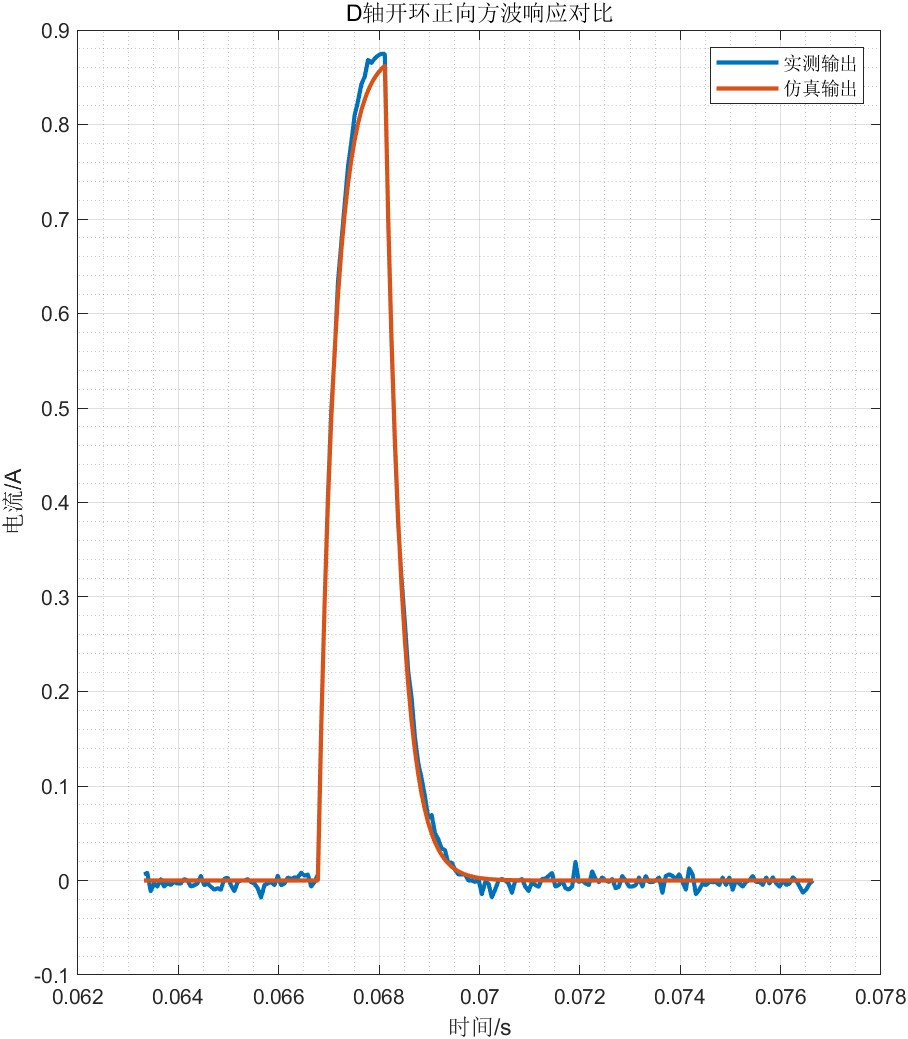
\includegraphics[width=\textwidth]
    {图片/D轴模型验证（正向）.jpg}
    \caption{D轴正向方波模型验证}
\end{figure}
\begin{figure}[H]
    \centering
    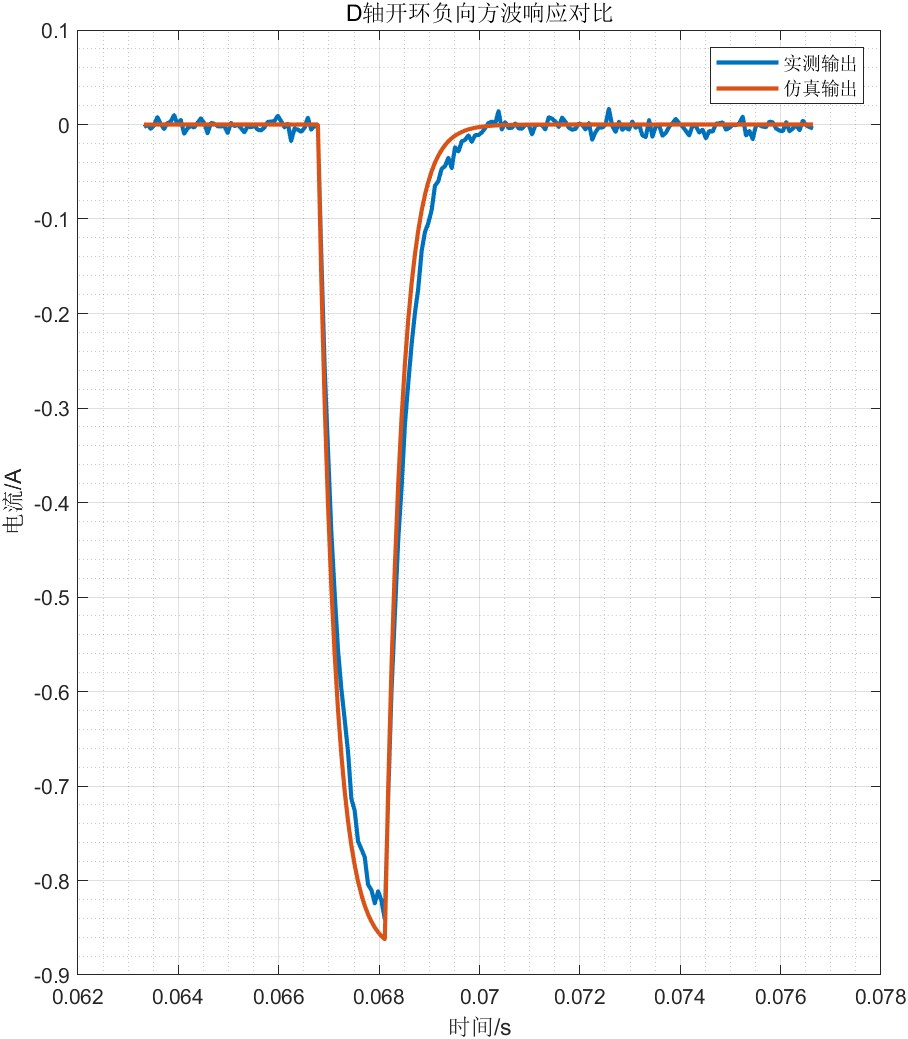
\includegraphics[width=\textwidth]
    {图片/D轴模型验证（负向）.jpg}
    \caption{D轴负向方波模型验证}
\end{figure}

根据响应曲线可以发现，D轴实测曲线和仿真曲线之间存在直流偏置（加性误差）。
尽管在程序初始化时于空载条件下测量了ADC偏置并加以扣除，但负载运行时电阻
因过电流温升导致的阻值漂移仍不可避免。一种简单的修正方法是将实测曲线整体
平移，使无激励区段的电流均值为零。误差修正前后的拟合程度如下表所示
\footnote{误差修正前后，相关系数保持不变，拟合优度升高，这是因为相关系数只衡量两者的线性相关性，
其中一组数据进行线性变换，不会影响两者的线性相关性，但却会影响两者的拟合优度，
这也是需要拟合优度作为另一个评价指标的原因。}。

\begin{table}[H]
    \centering
    \begin{tabular}{|c|c|c|c|c|}
        \hline
        \multirow{2}{*}{} & \multicolumn{2}{c|}{误差修正前} & \multicolumn{2}{c|}{误差修正后} \\
        \cline{2-5}
        & 相关系数 & 拟合优度 & 相关系数 & 拟合优度 \\
        \hline
        D轴正向 & 99.98599\(\%\) & 95.08867\(\%\) & 99.98599\(\%\) & 97.99685\(\%\) \\
        \hline
        D轴负向 & 99.87541\(\%\) & 93.25615\(\%\) & 99.87541\(\%\) & 94.83670\(\%\) \\
        \hline
    \end{tabular}
    \caption{D轴开环模型验证拟合程度表}
    \label{tab:D轴开环模型验证拟合程度表}
\end{table}

接下来对Q轴进行测试，结果如下。
\begin{figure}[H]
    \centering
    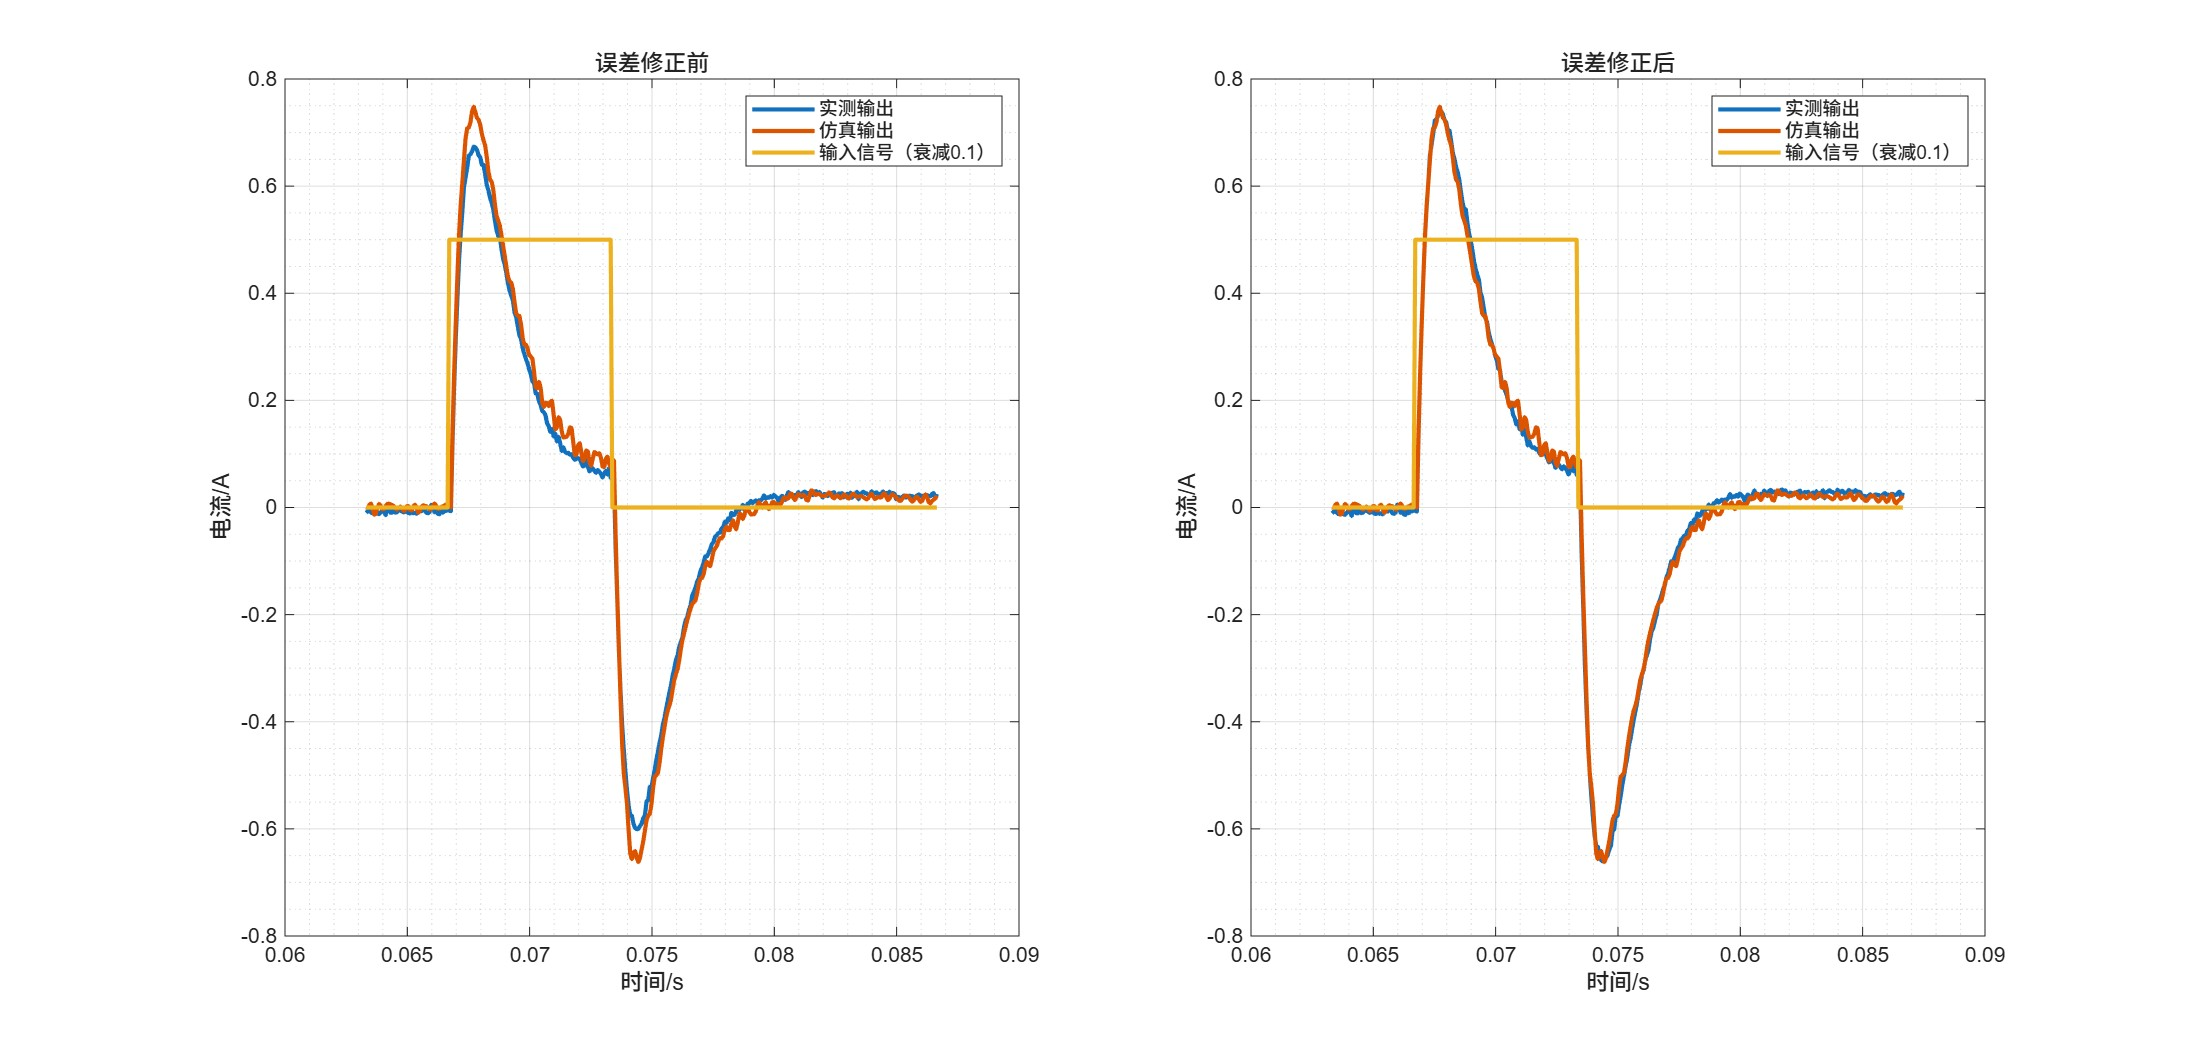
\includegraphics[width=\textwidth]
    {图片/Q轴模型验证（正向）.jpg}
    \caption{Q轴正向方波模型验证}
\end{figure}
\begin{figure}[H]
    \centering
    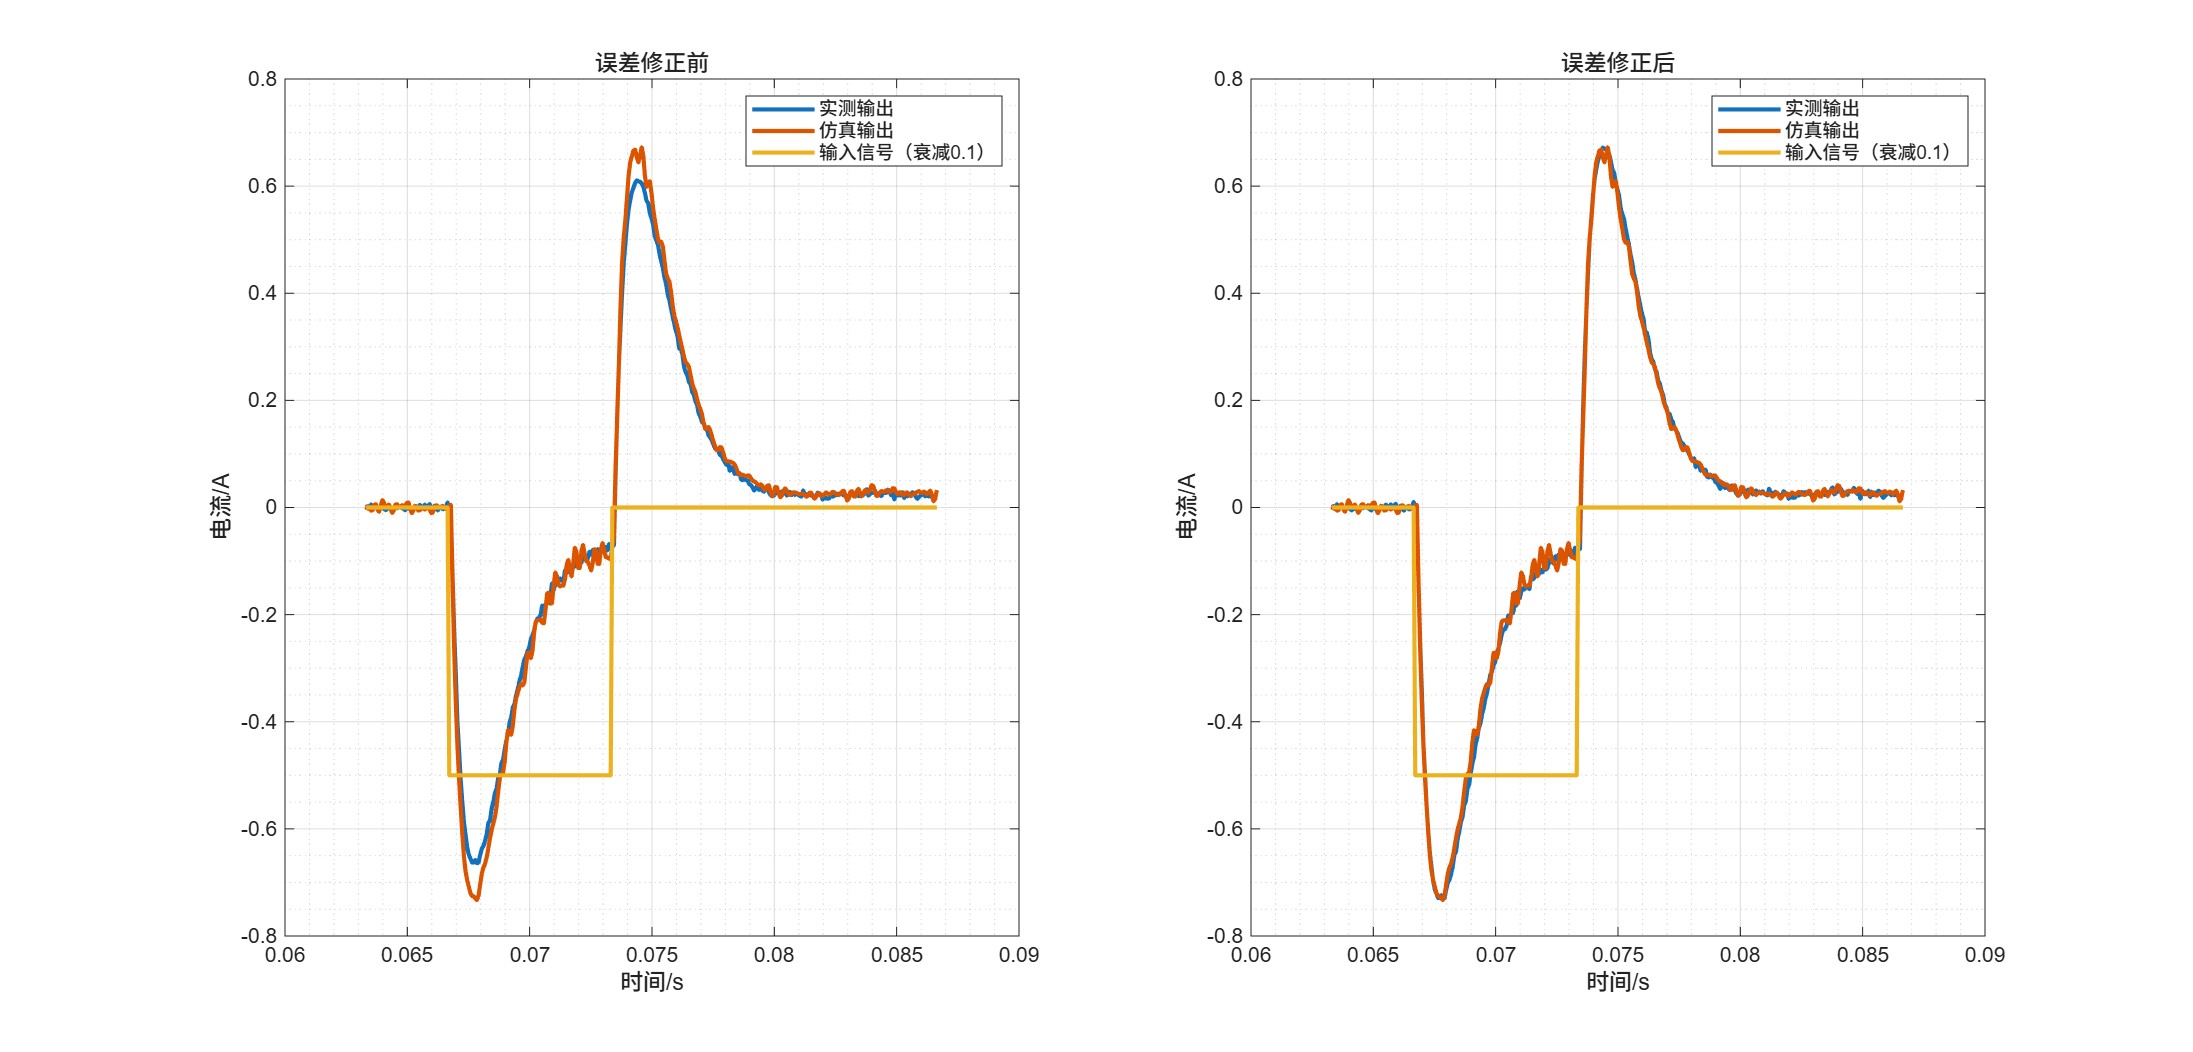
\includegraphics[width=\textwidth]
    {图片/Q轴模型验证（负向）.jpg}
    \caption{Q轴负向方波模型验证}
\end{figure}

与D轴的直流偏置加性误差不同，Q轴的实测曲线和仿真曲线之间存在增益偏差，属于乘性误差。
该误差的成因比D轴的加性误差成因更为复杂。D轴的等效RL电路模型无需反电动势补偿
（测试时保持\(i_q\approx 0\)即无交叉耦合），误差仅来源于电流采样链路的固定偏置。
而Q轴在空载测试时电机会因电磁转矩而转动，必须按
\(U_q'=U_q-\omega_e(L_d i_d+\psi_m)\)补偿反电动势才能将Q轴等效为RL电路。该补偿环节引入了
三个额外的误差源：
\begin{itemize}
    \item 永磁磁链\(\psi_m\)的辨识值存在误差，且\(\psi_m\)随温度升高而降低，实际运行中
    难以实时校准；
    \item 电角速度\(\omega_e\)的测量存在量化噪声和相位延迟，在方波跳变沿附近转速突变
    时尤为显著；
    \item 上述两项误差经乘积\(\omega_e\psi_m\)放大后注入等效电压\(U_q'\)，误差大小与
    转速成正比，而转速又与激励电流幅值正相关，因此误差呈现与信号幅值成比例的乘性特征。
\end{itemize}
一种简单的修正方法是对实测曲线施加一个缩放因子k，使得修正后两条曲线的峰值一致。误差修正前后的拟合程度如下表所示
\footnote{与加性误差同理，乘性误差修正前后相关系数保持不变（线性变换不改变线性相关程度），
而拟合优度因消除了增益偏差而升高。}。

\begin{table}[H]
    \centering
    \begin{tabular}{|c|c|c|c|c|}
        \hline
        \multirow{2}{*}{} & \multicolumn{2}{c|}{误差修正前} & \multicolumn{2}{c|}{误差修正后} \\
        \cline{2-5}
        & 相关系数 & 拟合优度 & 相关系数 & 拟合优度 \\
        \hline
        Q轴正向 & 99.86998\(\%\) & 90.06071\(\%\) & 99.86998\(\%\) & 94.71557\(\%\) \\
        \hline
        Q轴负向 & 99.91898\(\%\) & 91.09869\(\%\) & 99.91898\(\%\) & 95.53193\(\%\) \\
        \hline
    \end{tabular}
    \caption{Q轴开环模型验证拟合程度表}
    \label{tab:Q轴开环模型验证拟合程度表}
\end{table}

上述开环验证中，在误差修正前，无论D轴还是Q轴的拟合优度均超过90\(\%\)，
且修正后相关系数不变而拟合优度进一步提高，说明辨识模型能准确刻画电机的动态特性。
但从响应曲线也能看出，理想化DQ轴电路方程对现实电机行为的描述存在系统偏差
（D轴的加性偏置和Q轴的增益误差）。由于电流环采用带积分环节的控制器，积分作用保证了
闭环系统的稳态增益不受模型增益摄动的影响；但模型误差仍会在动态过程中影响
超调量和调节时间等暂态指标，这是后续控制器参数整定时需要关注的。